% arara: pdflatex
% arara: bibtex
% arara: pdflatex
% arara: pdflatex
%
% Basierend auf der Vorlage des MNM-Teams
% - optimiert für die Arbeit mit gängigen LaTeX-Editoren
% - funktioniert ohne Makefile und Anpassungen der LaTeX-Verzeichnisstruktur
% - verwendet Komaskript für ein (nach europäischen Gepflogenheiten) schöneres Layout
%
% v1, 2007 (Michael Brenner)
% v1.1, 2012 (Michael Brenner)
% v1.2, 2017 (Michael Brenner)
% v1.2.1, 2017 (Benjamin Schnoy)
% v1.3, 2018 (Michael Grabatin)
% Diese Version v2.0, 2020 (Henning Hontheim)

\documentclass[bibliography=totoc,listof=totoc,BCOR=5mm,DIV=12]{scrbook} % Rand für Bindung: 5mm / falls Index verwendet, ergänze "index=totoc" zu den Optionen
%\usepackage{ngerman}
\usepackage[ngerman]{babel}
\usepackage[utf8]{inputenc}
\usepackage[T1]{fontenc}
\usepackage{latexsym}
\usepackage{amsmath,amsfonts,amssymb,amsthm,amscd}
\usepackage{dsfont}
\usepackage{graphicx}
\usepackage[flushleft]{paralist} 
\usepackage[dvipsnames]{xcolor} 
\usepackage[all]{xy}
\usepackage{makeidx}
\usepackage{graphicx}
\usepackage{verbatim}
\usepackage{pdfpages}
\usepackage[printonlyused]{acronym} % http://namsu.de/Extra/pakete/Acronym.pdf %% footnote, nohyperlinks
\usepackage[inline]{enumitem}
\usepackage{csquotes}
\usepackage{makecell}
\usepackage{booktabs}

\usepackage{pgf}
\usepackage{tikz}
\usepackage{pgfplots}
\usepackage{mathrsfs}
\usepackage{adjustbox}
\usepackage{float}
\usepackage{longtable}

% \usepackage{showframe}
 
\usepackage{scrhack}

\usetikzlibrary{calc,shapes,arrows,positioning}
\pgfplotsset{compat=1.15}

\usepackage{listings}

\definecolor{cLightPlain}{HTML}{000000}
\definecolor{cLightKeyword}{HTML}{9B2393}
\definecolor{cLightComment}{HTML}{5D6C79}
\definecolor{cLightString}{HTML}{C41A16}
\definecolor{cLightNumber}{HTML}{1C00CF}
\definecolor{cLightBackground}{HTML}{FFFFFF}

\usepackage{pifont}
\usepackage[binary-units=true]{siunitx}

\newcounter{lstannotation}
\setcounter{lstannotation}{0}
\renewcommand{\thelstannotation}{\ding{\number\numexpr181+\arabic{lstannotation}}}
\newcommand{\annotation}[1]{\refstepcounter{lstannotation}\label{#1}\thelstannotation}

\lstdefinelanguage{mySwift}{
	language=Swift,
	morekeywords={
%		@Published,
%		@State,
%		@Binding,
%		@ObservedObject,
%		@EnvironmentObject,
		some
	}
}

\lstdefinestyle{mySwiftStyle}{
	language=mySwift,
	numbers=left,
	numbersep=5pt,
	breaklines=true,
	showstringspaces=false,
	frame=l ,
	xleftmargin=15pt,
	xrightmargin=15pt,
	basicstyle=\ttfamily\scriptsize\color{cLightPlain},
	stepnumber=1,
	keywordstyle=\color{cLightKeyword},
	commentstyle=\color{cLightComment},
	stringstyle=\color{cLightString},
	numberstyle=\tiny\color{cLightNumber},
	backgroundcolor=\color{cLightBackground},
	escapeinside={/*!}{!*/}
}

\lstset{style=mySwiftStyle}

%\usepackage{url}
\usepackage{hyperref}
%\usepackage[parfill]{parskip}

\newcommand{\singlequotes}[1]{\glq#1\grq}
\newcommand{\doublequotes}[1]{\glqq#1\grqq}

\newcommand{\R}{\mathds{R}}
\newcommand{\Z}{\mathds{Z}}
\newcommand{\N}{\mathds{N}}
\newcommand{\Q}{\mathds{Q}}
\newcommand{\K}{\mathds{K}}
\newcommand{\C}{\mathds{C}}
\newcommand{\B}{\mathds{B}}
\newcommand{\F}{\mathds{F}}
\newcommand{\p}{\mathfrak{p}}
\newcommand{\Pot}{\mathcal{P}}
\newcommand{\id}{\textup{id}}
\newcommand{\Ker}{\textup{Ker}}
\newcommand{\Image}{\textup{Im}}
\newcommand{\la}{\langle}
\newcommand{\ra}{\rangle}

\newtheorem{lemma}{Lemma}[section]
\newtheorem{prop}[lemma]{Proposition}
\newtheorem{defprop}[lemma]{Definition and Proposition}
\newtheorem{satz}[lemma]{Satz}
\newtheorem{thm}[lemma]{Theorem} 
\newtheorem{kor}[lemma]{Korollar} 
\newtheorem{folg}[lemma]{Folgerung}
\newtheorem{verm}[lemma]{Vermutung}
\newenvironment{bew}{\begin{proof}[Beweis]}{\end{proof}}
\theoremstyle{definition} 
\newtheorem{def1}[lemma]{Definition} 
\newtheorem{bem}[lemma]{Bemerkung}
\newtheorem{ford}[lemma]{Forderung}
\newtheorem{bsp}[lemma]{Beispiel}
\newtheorem{notation}[lemma]{Notation}

\let\svthefootnote\thefootnote
\newcommand\blankfootnote[1]{%
	\begin{NoHyper}
		\let\thefootnote\relax\footnotetext{#1}%
		\let\thefootnote\svthefootnote%
	\end{NoHyper}
}

%\newenvironment{packed}{
%	\begin{itemize}
%		\setlength{\itemsep}{0pt}
%		\setlength{\parskip}{0pt}
%		\setlength{\parsep}{0pt}
%	}{\end{itemize}}

%% Old version for BibTeX
%\usepackage{natbib}
%\setcitestyle{authoryear,square,numbers,longnamesfirst}
%\bibliographystyle{abbrvnat} % alphadin, plainnat, bst, nature, agms, dcu, kluwer, agu, egu, cospar, plain

\usepackage[
	backend=biber,
	style=numeric,
	citestyle=numeric,
	maxbibnames=9,
	maxcitenames=2,
%	maxnames=2
%	uniquename=false
]{biblatex}

%% Ignore specific fields...
%% https://tex.stackexchange.com/questions/174030/misplaced-alignment-tab-character-error-when-citing-a-particular-entry
%\DeclareSourcemap{
%	\maps[datatype=bibtex]{
%		\map{
%			\step[fieldsource=doi,null]
%			\step[fieldset=url,null]
%			\step[fieldset=urldate,null]
%		}  
%	}
%}

% @uri[reference][Change german u.a. to et al.]: https://tex.stackexchange.com/questions/236854/changing-u-a-of-german-to-et-al#386940
\DefineBibliographyStrings{ngerman}{
	andothers = {{et\,al\adddot}},
}

\addbibresource{./bibliography/bibliography.bib}

\setcounter{tocdepth}{3}

\graphicspath{{./images/}}

\hyphenation{Hu-man}
\hyphenation{cen-tred}
\hyphenation{Hu-man-cen-tred}

\hyphenation{Ma-nage-ment}
\hyphenation{Ma-nage-ment-agent}
\hyphenation{Ma-nage-ment-agent-en}
\hyphenation{Ma-nage-ment-ar-chi-tek-tur}
\hyphenation{Ma-nage-ment-ar-chi-tek-tu-ren}
\hyphenation{Ma-nage-ment-an-wen-dung}
\hyphenation{Ma-nage-ment-an-wen-dung-en}
\hyphenation{Ma-nage-ment-an-for-der-ung}
\hyphenation{Ma-nage-ment-funk-ti-on}
\hyphenation{Ma-nage-ment-funk-ti-onen}
\hyphenation{Ma-nage-ment-kon-zep-te}
\hyphenation{Ma-nage-ment-res-source}
\hyphenation{Ma-nage-ment-in-for-ma-ti-on}
\hyphenation{Ma-nage-ment-res-sour-cen}
\hyphenation{ma-nage-ment-re-le-vante}
\hyphenation{ma-nage-ment-sy-stem}
\hyphenation{ma-nage-ment-sy-steme}
\hyphenation{Ma-nage-ment-in-stru-men-tie-rung}
\hyphenation{Ma-nage-ment-platt-form}
\hyphenation{Sys-te-men}
\hyphenation{Sys-tem-um-ge-bun-gen}
\hyphenation{Sys-tem-ma-nage-ment}
\hyphenation{DHCP}
\hyphenation{Ma-nage-ment-diszi-plinen}
\hyphenation{System-management-architekturen}
\hyphenation{Verwendungs-nachweise}
\hyphenation{Video-einricht-ungen}
\hyphenation{Res-source}
\hyphenation{Res-sourcen}
\hyphenation{Grund-anwendung}
\hyphenation{Grund-anwendungen}
\hyphenation{Basis-anwendung}
\hyphenation{Core}
\hyphenation{Kom-mu-ni-ka-ti-on}
\hyphenation{De-sign-ent-schei-dung}
\hyphenation{Sprung-ad-res-sen}
\hyphenation{Klas-si-fi-ka-ti-on}
\hyphenation{Schreib-recht}
\hyphenation{Be-nut-zer-zer-ti-fi-kat}
\hyphenation{Bau-stein-ent-wi-ckler}
\hyphenation{ad-mi-ni-stra-ti-ve}


 \hypersetup{pdftitle={Smartwatch-basierte Benutzerschnittstelle zur Identifikation im urbanen Raum},pdfauthor={Henning Hontheim}}

\begin{document}

% ---------------------------------------------------------------
\frontmatter
    %%%%%%%%%%%%%%%%%%%%%%%%%%%%%%%
% erste Seite
% Deckblatt

\newcommand{\content}{
	\vspace*{1cm}
	
	
\includegraphics[width=0.6\textwidth]{./images/unibw_athene_neu}
	
	\vspace{1.5cm}
	{\Huge %
		% Titel der Arbeit, nicht benötigte Zeilen auskommentieren
		\textbf{Smartwatch-basierte Benutzerschnittstelle zur Identifikation im urbanen Raum}\\ %
		% \textbf{}\\ %
	} %
	\vspace{1.5cm}
	
	
	{\Large
		Bachelorarbeit von\\
		Henning Hontheim\\
		Matrikelnummer: \texttt{1174049}\\
}}


\thispagestyle{empty}

\begin{center}

\content

\vspace{1cm}
%Entwurf vom \today\\ % TODO: Für finale Version entfernen!
%\input{./misc/version}

\vfill

{\Large %
Universität der Bundeswehr München\\
Fakultät für Informatik\\
}


\end{center}

\newpage

%%%%%%%%%%%%%%%%%%%%%%%%%%%%%%%
% zweite Seite
% (Rückseite der ersten Seite)

\thispagestyle{empty}
\cleardoublepage

%%%%%%%%%%%%%%%%%%%%%%%%%%%%%%%
% dritte Seite (Kopie der ersten)
% erste Seite der Arbeit

\thispagestyle{empty}

\begin{center}
	
	\content
	
	\vspace{2cm}
	
	\parbox{1cm}{
\begin{large}
\begin{tabbing}
Aufgabensteller: \hspace{.5cm} \=Prof.\ Dr.\ Michael Koch\\[2mm]
Zweitprüfer: \>Prof.\ Dr.\ Gunnar Teege\\[2mm]
Betreuer:
%\>Betreuer 1\\ % alphabetische Reihenfolge (Nachname)
%\>Betreuer 2\\
%\>Externer Betreuer 1 (Firma)\\[5mm]
\>Julian Fietkau\\[5mm]
Abgabetermin: \> 2. Juni 2020\\
\end{tabbing}
\end{large}}\\
\vspace{5mm}

\vfill

{\Large %
Universität der Bundeswehr München\\
Fakultät für Informatik\\
}

\end{center}

    \thispagestyle{empty}
    \cleardoublepage
    \thispagestyle{empty}
    \tableofcontents

% ---------------------------------------------------------------
\mainmatter

    \chapter{Einleitung}

Zwischen 2015 und 2050 wird die Zahl der Menschen, die älter als 60 Jahre sind, von 900 Millionen auf 2 Milliarden steigen. Dies entspricht einem Anstieg von $ 12 \% $ auf $ 22 \% $ der gesamten Weltbevölkerung\footnote{\url{https://www.who.int/features/factfiles/ageing/en/}}.

Werden ältere Personen mit neuen Technologien, wie etwa Smartphones, konfrontiert, herrscht oft eine gewisse Abneigung. Der häufigste Grund sind Bedenken hinsichtlich der Privatsphäre und des Datenschutzes. Ältere möchten oft nicht viel von sich preisgeben und haben Angst, dass diese Daten an die Öffentlichkeit gelangen könnten. Oft sind es aber auch mangelnde Kenntnisse und unzureichende Ausrüstung, die den Zugang zu diesen Technologien erschweren oder die Tatsache, dass Anwendungen selten an die Bedürfnisse und Interessen dieser angepasst sind \cite{Almeida:2015:Recommendations-for-the-Development-of-Web-Interfaces}\cite{Boll:2015:User-Interfaces-with}\cite{Leonardi:2010:An-Exploratory-Study-of-a-Touch-Based}.

Im Rahmen des Projekts \doublequotes{UrbanLife+}\footnote{\url{https://www.urbanlifeplus.de}} der Universität der Bundeswehr München, wird versucht die Teilhabe von Senioren im öffentlichen Raum zu verbessern. Mit dieser Arbeit möchten wir untersuchen, welche Richtlinien es bei Benutzerschnittstellen für ältere Personen gibt, indem wir bereits existierende Arbeiten analysieren und daraus Best Practices ableiten.

Im Anschlus soll eine mobile Anwendung für das iPhone und die Apple Watch entwickelt werden, die eine Identifikation im urbanen Raum über \emph{Bluetooth Low Energy} ermöglicht.

Allein aus Gr"unden der Lesbarkeit wird auf die gleichzeitige Verwendung mehrerer geschlechtsspezifischer Sprachformen verzichtet. S"amtliche Personenbezeichnungen gelten f"ur alle Geschlechter.
    \chapter{Stand der Wissenschaft und verwandte Arbeiten}

In diesem Kapitel wollen wir uns einen Überblick über den aktuellen Stand der Forschung verschaffen. Es wird untersucht, welche Erkenntnisse es zum Design von \acp{UI} für ältere Personen gibt und welche Richtlinien sich daraus ableiten lassen, die bei der Entwicklung einer Touch-basierten Anwendung beachtet werden sollten. Zudem wird gezeigt, welche Ergebnisse es hinsichtlich der Benutzung von Smartwatches durch ältere Personen gibt. Auch eine Unterstützung durch Bluetooth wird vorgestellt.

\section{User Interfaces für ältere Menschen}\label{sec:guidelines}

Mit zunehmendem Alter nimmt eine Vielzahl von Fähigkeiten ab. Oft beeinträchtigt sind das Sehen und Hören, die Mobilität aber auch die kognitiven Fähigkeiten, die sich auf verschiedene Aspekte des Alltagslebens auswirken. Eine uneingeschränkte Interaktion mit Smartphones oder anderen Geräten, kann nur durch Unterstützung erfolgen \cite{Almeida:2015:Recommendations-for-the-Development-of-Web-Interfaces}\cite{Diaz-Bossini:2014:Accessibility-to-Mobile-Interfaces}\cite{Huang:2016:Design-of-Smart-Watch}\cite{Salman:2018:Usability-Evaluation-of-the-Smartphone}\cite{Sin:2015:Evaluation-of-Wearable-Device}. Selbst Personen ohne Einschränkungen fällt es oft schwer, Touchscreens fehlerfrei zu bedienen. Auch wenn man vorsichtig ist, führt eine ungenaue Berührung manchmal dazu, dass eine falsche Funktion ausgeführt wird. Zudem kann eine Verwendung im Freien unmöglich sein, wenn der Inhalt des Displays in der Sonne schwer zu sehen ist \cite{Kivirinta:2013:The-Right-UI-for-Elderly-People;}.

\subsection{Universal Access}

Oft befassen sich Anwendungen, die für ältere Menschen bestimmt sind, ausschließlich mit der Barrierefreiheit. Ein wichtiger Punkt wird hierbei jedoch gerne übersehen: die Vertrautheit. Selbst wenn eine Anwendung so zugänglich wie nur möglich und somit sicherlich deutlich lesbarer und einfacher ist, kann diese doch noch so fremd sein. Sie bleibt ein Objekt, das von dem Wissen und der Kultur einer älteren Person weit entfernt ist \cite{Leonardi:2010:An-Exploratory-Study-of-a-Touch-Based}.

\doublequotes{Universal Access} oder \doublequotes{Universal Design} bezieht sich schon längst nicht mehr ausschließlich auf die Barrierefreiheit einer Anwendung und ist ein Ansatz, dieses Problem zu beheben, indem es diesen sieben Prinzipien folgt \cite{Kivirinta:2013:The-Right-UI-for-Elderly-People;}:

\begin{enumerate}%[nosep]
	\item \textbf{Einfache und intuitive Nutzung:} Leicht zu verstehen, unabhängig von Erfahrung, Wissen, Sprachkenntnissen oder dem Konzentrationsgrad des Nutzers.
	\item \textbf{Gerechte Nutzung:} Keine Nutzergruppe wird benachteiligt oder stigmatisiert.
	\item \textbf{Wahrnehmbare Informationen:} Vermittelt notwendige Informationen effektiv, ungeachtet der Umgebungsbedingungen oder sensorischen Fähigkeiten.
	\item \textbf{Fehlertoleranz:} Minimiert die Folgen versehentlicher oder unbeabsichtigter Handlungen.
	\item \textbf{Berücksichtigung von Vorlieben und Fähigkeiten:} Individuelle Anpassung an den Nutzer.
	\item \textbf{Geringe körperliche Anstrengung:} Kann effizient und bequem und mit einem Minimum an Ermüdung eingesetzt werden.
	\item \textbf{Freiraum für den Zugang und die Verwendung:} Angemessen hinsichtlich des Zugangs, der Erreichbarkeit und Nutzung unabhängig der Körpergröße, Körperhaltung oder Mobilität des Nutzers.
\end{enumerate}

Das Ziel ist es, ein Design zu entwickeln, das die Fähigkeiten aller Menschen berücksichtigt. Ein Design soll nicht bloß auf die Bedürfnisse einer ganz bestimmten Zielgruppe angepasst sein. Zur Inklusion aller Menschen braucht es einen Gestaltungsrahmen, der für alle gilt \cite{Marcus:2003:Universal-Ubiquitous-User-Interface}\cite{Stephanidis:2001:User-interfaces-for-all:}. 

\subsection{Human-centered Design}

Ein oft verwendeter Begriff ist der des \doublequotes{Human-centred Design} oder \doublequotes{User-centred Design} (dt. \doublequotes{mensch-/nutzerzentrierte Gestaltung}). Ein Ziel dessen ist es, dem Menschen die Kontrolle zu lassen. Doch je mehr Kontrolle man dem Nutzer lässt, umso weniger kann automatisiert werden. Auch führt eine Erhöhung der Privatsphäre dazu, dass ein System weniger Daten zur Verarbeitung hat und so \doublequotes{weniger intelligent} handeln kann. \doublequotes{Privacy by Design} bezeichnet ein Paradigma, bei dem der Datenschutz schon bei der Entwicklung eines Systems berücksichtigt wird \cite{Stephanidis:2001:User-interfaces-for-all:}\cite{Streitz:2018:Beyond-smart-only-cities:}.

Die Norm ISO 9241-210 \cite{ISO-Central-Secretary:2019:Ergonomics-of-human-system-interaction}, der Ersatz von ISO 13407, beschreibt den Prozess des \doublequotes{Human-centred Design}, der aus vier Phasen besteht:
\begin{enumerate*}[label=(\arabic*)]
	\item Verstehen des Nutzungskontextes,
	\item Festlegung der Nutzungsanforderungen,
	\item Entwurf von Gestaltungslösungen,
	\item Evaluation der Gestaltungslösungen.
\end{enumerate*}
\autoref{dia:human-centered-design-process} veranschaulicht diese Phasen graphisch. Bis ein optimales Endergebnis erzielt worden ist, werden diese iterativ durchlaufen \cite{Burmester::Design-Thinking--die-neue}\cite{Geis::Neue-ISO-9241-210-Prozess}.

\begin{figure}[p]
	% Template: http://www.texample.net/tikz/examples/control-system-principles/
	\begin{adjustbox}{center} % 	\begin{adjustbox}{scale=0.7,center}
		\begin{tikzpicture}[auto, node distance=1.75cm and,>=latex'] % Reihenfolge: vertical and horizontal!!
		
		\tikzstyle{all} = [draw, fill=blue!20, minimum height=3em, minimum width=6em, align=center]
		\tikzstyle{block} = [rectangle, all]
		\tikzstyle{round} = [ellipse, all]
		\tikzstyle{label} = [node distance=0.cm, align=right]
		
		\node [round, name=plan] {Den menschzentrierten\\Gestaltungsprozess planen};
		
		% Achtung! Andere Reihenfolge im Code (nicht im Zyklus!!)
		\node [block, below = of plan] (context) {Den Nutzungskontext\\verstehen und beschreiben};
		\node [block, below = of context] (evaluate) {Gestaltungslösungen aus der\\Benutzerperspektive evaluieren};
		\node [block, right = of evaluate] (develop) {Gestaltungslösungen entwickeln,\\die die Nutzungsanforderungen erfüllen};
		\node [block, above = of develop] (specify) {Die Nutzungsanforderungen\\spezifizieren};
		
		\node [round, below = of evaluate] (done) {Gestaltungslösung erfüllt die\\Nutzungsanforderungen};
		
		\draw [->] (plan) -- (context);
		\draw [->] (context) edge[bend left] (specify);
		\draw [->] (specify) edge[bend left] (develop);
		\draw [->] (develop) edge[bend left] (evaluate);
		\draw [->, dashed] (evaluate) edge[bend left] node[name=middle] {} (context);
		\draw [->, dashed] (evaluate) -- (specify);
		\draw [->, dashed] (evaluate.east) -- (develop.west);
		\draw [->] (evaluate) -- (done);
		
		\node [label, left = of middle] {Iteration, soweit\\Evaluierungsergebnisse\\Bedarf hierfür aufzeigen};
		
		\end{tikzpicture}
	\end{adjustbox}
	\caption{\label{dia:human-centered-design-process}Nach ISO 9241-210 definierter, iterativer Prozess zur Entwicklung eines Human-centred Designs \cite{Geis::Neue-ISO-9241-210-Prozess}.}
\end{figure}

\subsection{User Interface Richtlinien für ältere Personen}

Es existieren bereits einige Arbeiten, die sich mit Benutzerschnittstellen für ältere Personen beschäftigen. Um die Zugänglichkeit zu erhöhen wurden viele Richtlinien erarbeitet, die bei der Entwicklung einer mobilen Anwendung Berücksichtigung finden sollten. Im Idealfall sollte ein Nutzer eine Anwendung sofort verstehen und bedienen können \cite{Kivimaki:2013:User-Interface-for-Social}.

\subsubsection{Richtlinien nach Zaphiris et al. und der WAI}

Mithilfe einer Fokusgruppe, die auch ältere Personen beinhaltete, entwickelten \citeauthor{Zaphiris:2005:Age-Centered-Research-Based-Web-Design} Richtlinien für die Entwicklung von Websiten. Die dort entstandenen 38 Richtlinien wurden in elf Kategorien zusammengefasst, wie beispielsweise die \doublequotes{Benutzung von Grafiken} oder solche, die auf die kognitiven Fähigkeiten der Nutzer abgestimmt sind \cite{Zaphiris:2005:Age-Centered-Research-Based-Web-Design}\cite{Kurniawan:2005:Research-Derived-Web-Design-Guidelines}.
Einige dieser Richtlinien lassen auf die Entwicklung von Apps übertragen. Da manche Kategorien, wie \doublequotes{Links} oder \doublequotes{Suchmaschinen}, nicht infrage kommen, haben \textcite{Diaz-Bossini:2014:Accessibility-to-Mobile-Interfaces} diese Richtlinien für die Benutzung in Apps reduziert und sich auf sechs Kategorien mit 19 Richtlinien beschränkt. Tabelle \ref{tab:zaphiris-reduced-to-mobile} listet diese auf.

\begin{table}[p]
%		\centering
	\begin{itemize}[label={}]
		\item \textbf{Design interaktiver Elemente}
		\begin{itemize}[nosep]
			\item Verwenden Sie größere Elemente.
			\item Zeigen Sie eine klare Bestätigung bei Interaktion, die für ältere Personen sichtbar sein sollte, die Änderungen nicht unbedingt bemerken müssen.
			\item Von einem Älteren sollte nicht erwartet werden, dass er doppelt klicken muss.
		\end{itemize}
			\item \textbf{Verwendung von Grafiken}
		\begin{itemize}[nosep]
			\item Grafiken sollten relevant sein und nicht zur Dekoration dienen. Verwenden Sie keine Animationen.
			\item Bilder sollten Beschreibungen zur Verfügung stellen.
			\item Icons sollten einfach, aber aussagekräftig sein.
		\end{itemize}
			\item \textbf{Funktionen des Browser-Fensters}
		\begin{itemize}[nosep]
			\item Vermeiden Sie Scrollbalken.
			\item Stellen Sie nur ein offenes Fenster dar. Pop-ups, animierte Werbung oder Überlappung mehrerer Fenster sollten vermieden werden.
		\end{itemize}
			\item \textbf{Gestaltung des Inhalts}
		\begin{itemize}[nosep]
			\item Nutzen Sie einfache und verständliche Sprache.
			\item Vermeiden Sie unwichtige Informationen.
			\item Wichtige Informationen sollten hervorgehoben werden.
			\item Informationen sollten vor allem im Zentrum positioniert werden.
			\item Das Bildschirmlayout, die Navigation und die verwendete Terminologie sollten einfach, klar und konsistent sein.
		\end{itemize}
			\item \textbf{Anpassung an kognitive Fähigkeiten der Nutzer}
		\begin{itemize}[nosep]
			\item Stellen Sie ausreichend Zeit zum Lesen von Informationen zur Verfügung.
			\item Reduzieren Sie die Beanspruchung des Gedächtnisses. Erkennen und unterstützen Sie das Verhalten der Nutzer und stellen Sie so weniger Wahlmöglichkeiten zur Verfügung.
		\end{itemize}
			\item \textbf{Verwendung von Farben und Hintergründen}
		\begin{itemize}[nosep]
			\item Farben sollten zurückhaltend verwendet werden.
			\item Blaue und grüne Farbtöne sollten vermieden werden.
			\item Hintergründe sollten nicht rein weiß sein. Die Helligkeit zwischen verschiedenen Bildschirmen sollte sich nicht schnell ändern. Stellen Sie Vorder- und Hintergründe kontrastreich dar. Vermeiden Sie farbigen Text auf farbigen Hintergründen.
			\item Bei Verwendung von Farben, sollten Sie auch schwarz und weiß verwenden.
		\end{itemize}
	\end{itemize}
	\caption{\label{tab:zaphiris-reduced-to-mobile}Von \textcite{Diaz-Bossini:2014:Accessibility-to-Mobile-Interfaces} gekürzte Richtlinien nach \textcite{Zaphiris:2005:Age-Centered-Research-Based-Web-Design}. Aus dem Englischen übersetzt.}
\end{table}

Auch die \ac{WAI} des \ac{W3C} hat für die Entwicklung von Web-Anwendungen Best Practices veröffentlicht, die \doublequotes{\ac{MWBP}} und die \doublequotes{\ac{MWABP}}. Diese sind Anpassungen der \doublequotes{\ac{WCAG}}, die für die Entwicklung von Webseiten gelten \cite{Web-Accessibility-Initiative::Older-Users-and-Web-Accessibility:}. Anders als die \ac{WCAG} sind diese jedoch keine Richtlinien.
Eingeteilt sind diese in vier Kategorien:
\begin{enumerate*}[label=(\arabic*)]
	\item Wahrnehmbarkeit,
	\item Bedienbarkeit,
	\item Verständlichkeit,
	\item Robustheit.
\end{enumerate*}
Letztere wurde von \citeauthor{Diaz-Bossini:2014:Accessibility-to-Mobile-Interfaces} nicht berücksichtigt, da diese nicht auf native Anwendungen anwendbar seien.

\citeauthor{Diaz-Bossini:2014:Accessibility-to-Mobile-Interfaces} haben schließlich anhand der gekürzten Richtlinien von \citeauthor{Zaphiris:2005:Age-Centered-Research-Based-Web-Design} (\autoref{tab:zaphiris-reduced-to-mobile}), den Best Practices der \ac{WAI} \cite{Web-Accessibility-Initiative::Older-Users-and-Web-Accessibility:}\cite{Diaz-Bossini:2014:Accessibility-to-Mobile-Interfaces} und den \citetitle{Google-Inc.::Android-Accessibility-Practices} von \textcite{Google-Inc.::Android-Accessibility-Practices} drei native Android-Apps evaluiert. Keine dieser Apps erfüllt alle Richtlinien und Best Practices vollständig. Manchen Apps fehlt es beispielsweise an Unterstützung zur Sprachausgabe einer Beschreibung von Bildern, andere fokussieren sich ausschließlich auf Unterstützung sehbeeinträchtigter Personen \cite{Diaz-Bossini:2014:Accessibility-to-Mobile-Interfaces}.

\subsubsection{Richtlinien nach den SMASH}

Einen anderen Ansatz der Bewertung von \aclp{UI} verfolgen \textcite{Salman:2018:Usability-Evaluation-of-the-Smartphone}mit den von \textcite{Inostroza:2016:Developing-SMASH:-A-set-of-SMArtphones} entwickelten \doublequotes{\acl{SMASH}} (\acs{SMASH}). Diese bestehen aus 12 Heuristiken, die in \autoref{tab:smash-list} aufgelistet sind. \citeauthor{Salman:2018:Usability-Evaluation-of-the-Smartphone} nutzen einen formativen Ansatz zur Bestimmung der Benutzbarkeit (Usability) der Benutzeroberfläche eines Android Smartphones (Version 6.0.1 \doublequotes{Marshmallow}). Anders als der summative Ansatz, der sich auf die Messung der Effektivität, Effizienz und Zufriedenheit bezieht, hängt beim formativen Ansatz das Vorhandensein der Benutzbarkeit von der Abwesenheit von Usability-Problemen ab \cite{Lewis:2014:Usability:-Lessons-Learned}. Diese Probleme sollen mithilfe der \ac{SMASH} gefunden werden.

\begin{table}[H]
	\begin{enumerate}[label={SMASH\arabic*.},leftmargin=7em,nosep]
		\item Sichtbarkeit des Systemstatus.
		\item Übereinstimmung zwischen System und der realen Welt.
		\item Kontrolle und Freiheiten des Benutzers.
		\item Einheitlichkeit und Standards.
		\item Fehlervermeidung.
		\item Keine Überanstrengung des Gedächtnisses.
		\item Anpassungen und Shortcuts.
		\item Effizienz hinsichtlich Nutzung und Leistung.
		\item Ästhetisches und minimalistisches Design.
		\item Anwendern helfen, Fehler zu erkennen, zu diagnostizieren und zu beheben.	
		\item Hilfe und Dokumentation.
		\item Körperliche Interaktion und Ergonomie.
	\end{enumerate}
	\caption{\label{tab:smash-list}Liste der \acf{SMASH}\cite{Inostroza:2016:Developing-SMASH:-A-set-of-SMArtphones}. Aus dem Englischen übersetzt.}
\end{table}


Nach Analyse des Betriebssystems durch von \citeauthor{Salman:2018:Usability-Evaluation-of-the-Smartphone} ausgesuchten Experten, wurden 27 Verletzungen gegen die \ac{SMASH} vorhergesagt. Mit jeweils sieben Verstößen sind SMASH6 und SMASH2 Spitzenreiter, gefolgt von SMASH11 (vier Verstöße), SMASH4 (drei Verstöße) und sechs weiteren Verstößen. $ 79.17 \% $ dieser vorhergesagten Verletzungen wurden im Rahmen der formativen Analyse durch einen anschließenden Test mit älteren Personen (über 60 Jahre alt) bestätigt. Dieser Test offenbarte fünf weitere Verstöße, die nicht vorhergesagt wurden. Schließlich wurden alle Verstöße in vier Kategorien eingeteilt (Erscheinungsbild, verwendete Sprache, Dialog mit dem Anwender und Informationsverwaltung) und Gestaltungslösungen dagegen vorgeschlagen. Diese lassen sich in \autoref{tab:smash-conforming-design-solutions} finden. Beispiele in \cite{Salman:2018:Usability-Evaluation-of-the-Smartphone}.

\begin{table}[p]
	\small
%	\renewcommand{\tablename}{Tab.}
%	\centering
	\begin{itemize}[label={}]
%		\setlength{\parskip}{0pt}
		\item \textbf{Erscheinungsbild}
		\begin{itemize}[nosep]
			\item Stellen Sie Elemente durch besser sichtbare Farben und in einer auffälligen Größe dar.
			\item Platzieren Sie Elemente, insbesondere wichtige, im sichtbaren Bereich. Dieser sollte vorzugsweise mit dem Daumen zu erreichen sein.
			\item Unterscheiden Sie deutlich zwischen interaktiven und nicht-interaktiven Elementen und ergänzen Sie die interaktiven mit einem Label.
			\item Wahren Sie einen deutlichen Kontrast zwischen Elementen und deren Hintergrund.
			\item Nutzen Sie aussagekräftige Icons, die konsistent verwendet werden.
			\item Passen Sie das Design an die Erfahrungen der Älteren an.
			\item Vermeiden Sie ungewohnte Designs.
		\end{itemize}
		\item \textbf{Verwendete Sprache}
		\begin{itemize}[nosep]
			\item Vermeiden Sie mehrdeutige Begriffe. Passen Sie sich dem Vokabular der Älteren an.
			\item Ergänzen Sie Text, wo angebracht, mit Icons.
			\item Vermeiden Sie die Nutzung technischer Begriffe, wie beispielsweise \doublequotes{PIN}. Wo notwendig helfen Sie dem Nutzer, diese zu verstehen.
			\item Verwenden Sie eindeutige Begriffe für die Label von UI-Elementen.
			\item Halten Sie die verwendete Terminologie konsistent.
		\end{itemize}
		\item \textbf{Dialog mit dem Anwender}
		\begin{itemize}[nosep]
			\item Die wichtigste Geste zur Interaktion mit der Benutzeroberfläche sollte eine einfache Berührung sein (Single Tap).
			\item Wenn Sie knifflige Gesten wie beispielsweise \doublequotes{Drag and Drop} oder \doublequotes{Tap and Hold} nutzen, bieten Sie älteren Menschen eine alternative Möglichkeit, die Aufgabe auszuführen.
			\item Zeigen Sie für jede destruktive Aktion eine Bestätigungsmeldung, die die Folge beschreibt.
			\item Machen Sie älteren Menschen durch unmittelbares Feedback deutlich, wann eine Aktion ausgeführt wurde.
			\item Unterstützen Sie den Nutzer durch zusätzliche Feedbacks, wie beispielsweise Audio-Feedbacks.
			\item Erlauben Sie älteren Benutzern, die genutzten Ressourcen zu verwalten. Führen Sie Funktionen in kurzen und einfachen Schritten aus.
			\item Gewährleisten Sie die gleiche, konsistente Systemreaktion auf die gleiche Benutzeraktion.
		\end{itemize}
		\item \textbf{Informationsverwaltung}
		\begin{itemize}[nosep]
			\item Platzieren Sie die wichtigsten Informationen im Vordergrund.
			\item Gruppieren Sie unwichtigere Informationen.
			\item Vermeiden Sie unwichtige Informationen.
			\item Stellen Sie ein Widget zur Verfügung, das die empfangenen Warnmeldungen und Benachrichtigungen sammelt und dem Benutzer hilft, diese zu verwalten.
			\item Geben Sie Hilfestellungen zur aktuellen Tätigkeit des Nutzers und zeigen Sie die notwendigen Schritte, die zu befolgen sind.
			\item Ergänzen Sie die Benutzeroberfläche mit visuellen Hinweisen, um älteren Menschen zu helfen, sich versteckter Inhalte bewusst zu werden.
			\item Helfen Sie mit Tooltips, wenn beispielsweise eine bestimmte Geste zur Ausführung einer bestimmten Aufgabe erforderlich ist.
		\end{itemize}
	\end{itemize}
	\caption{\label{tab:smash-conforming-design-solutions}Von \textcite{Salman:2018:Usability-Evaluation-of-the-Smartphone} entwickelte Gestaltungslösungen zur Einhaltung der \acf{SMASH} von \textcite{Inostroza:2016:Developing-SMASH:-A-set-of-SMArtphones}. Aus dem Englischen übersetzt.}
\end{table}

\subsection{Weitere Erkenntnisse}

Zusätzlich zu den bereits genannten Richtlinien und Empfehlungen existieren weitere Arbeiten, die sich ebenfalls mit \aclp{UI} für Ältere beschäftigen. Da diese mit den bereits erwähnten Arbeiten in vielen Punkten übereinstimmen, wird im Folgenden nur auf neue Erkenntnisse oder Unterschiede eingegangen.

\paragraph{Animationen}
Um den Nutzer über asynchrone Ereignisse oder Hintergrundaktivitäten zu informieren, sind Animation hilfreich. Nach Erfahrung von \textcite{Leonardi:2010:An-Exploratory-Study-of-a-Touch-Based} reichen diese allerdings nicht notwendigerweise aus, um der Aktivitäten auch tatsächlich bewusst zu werden.

\paragraph{Erster Start der Anwendung}
Stellen Sie die Hauptfunktionen beim ersten Starten der Anwendung vor und helfen Sie dem Nutzer, sich zurechtzufinden \cite{Almeida:2015:Recommendations-for-the-Development-of-Web-Interfaces}.

\paragraph{Feedback}
Geben Sie visuelles, akustisches oder auch haptisches Feedback bei Interaktion mit den Elementen \cite{Almeida:2015:Recommendations-for-the-Development-of-Web-Interfaces}.

\paragraph{Gesten}
Halten Sie Gesten einfach und vermeiden Sie solche, die mehr als zwei Finger benötigen oder den Einsatz beider Hände erfordern \cite{Almeida:2015:Recommendations-for-the-Development-of-Web-Interfaces}. Problematisch ist der \doublequotes{Double Tap}, da zwischen den beiden Berührungen zu viel Zeit liegen kann, so dass die Geste als zwei einfache Interaktionen interpretiert werden könnte \cite{Boll:2015:User-Interfaces-with}.

Nicht zu vernachlässigen ist auch, dass ein einfacher \doublequotes{Tap}, der sehr langsam ausgeführt wird, unter Umständen als \doublequotes{Drag and Drop} interpretiert werden kann, wenn der Finger leicht zur Seite bewegt wird. Um einen gewollten \doublequotes{Drag and Drop} auszuführen muss ersichtlich sein, dass ein Element auch verschoben werden kann \cite{Leonardi:2010:An-Exploratory-Study-of-a-Touch-Based}.

\paragraph{Layout von Elementen}
Hinsichtlich der Mindestgröße von Elementen, gibt es verschiedene Erkenntnisse. Empfehlungen reichen von Durchmessern mit 9 mm\cite{Burkhard:2012:Evaluating-Touchscreen-Interfaces}, über 12 mm\cite{Guerreiro:2010:Towards-Accessible-Touch}, bis hin zu 16.5 mm\cite{Murata:2005:Usability-of-Touch-Panel-Interfaces}. Zwischen verschiedenen Interface-Elementen sollte ein Mindestabstand von 44 px eingehalten werden, damit diese auch gut erreicht werden können \cite{Almeida:2015:Recommendations-for-the-Development-of-Web-Interfaces}.

\paragraph{Schrift}
Nutzen Sie serifenlose Schriftarten\footnote{\textsf{Ein Beispiel für eine serifenlose Schriftart ist dieser Satz.}} für Displays \cite{Almeida:2015:Recommendations-for-the-Development-of-Web-Interfaces}\cite{Darroch:2005:The-Effect-of-Age-and-Font-Size}. Verwenden Sie eine Schriftgröße, die in etwa $ 3.5 $ Millimetern auf dem Display entspricht \cite{Darroch:2005:The-Effect-of-Age-and-Font-Size}.

\paragraph{Sofortige Aktualisierung}
Vermeiden Sie Funktionen, die die angezeigten Informationen bei jeder Interaktion ändern, wie beispielsweise Filter für Listen und Autovervollständigungen \cite{Almeida:2015:Recommendations-for-the-Development-of-Web-Interfaces}.

\section{Wearables und Smartwatches}

Tragbare Geräte, wie Smartwatches, erfreuen sich immer größerer Beliebtheit. Doch ein Problem, welches diese mit sich bringen, ist die Tatsache, dass das Display deutlich kleiner ist, als das eines Smartphones. Bei Verwendung dieser kleinen Geräte durch ältere Menschen, kann es aufgrund der bereits erwähnten körperlichen und geistigen Einschränkungen, zu vielen Problemen kommen \cite{Huang:2016:Design-of-Smart-Watch}.

\textcite{Fang:2014:A-New-Smart-Wearable-Device} haben sich mit Wearables für ältere Menschen auseinandergesetzt. Ein Ziel ist es gewesen, das Unbehagen zu reduzieren, das durch das Tragen eines Gerätes hervorgerufen werden kann. Untersucht wurden drei Positionen, an denen ein Gerät getragen werden kann: das Handgelenk, der Oberarm und der Nacken.

Sie sind zu dem Ergebnis gekommen, dass das Handgelenk am besten geeignet ist. Die Angst, die hervorgerufen werden kann, wenn ein Gerät am Nacken getragen wird, ist am Handgelenk deutlich geringer. Ein weiterer Vorteil des Tragens am Handgelenk, ist die bessere Lesbarkeit im Vergleich zum Oberarm. Es ist wesentlich einfacher, den Arm anzuheben, um einen guten Betrachtungswinkel auf ein Display zu bekommen, als den Kopf in Richtung des Oberarms zu drehen.

Dadurch, dass ein Träger eine Armbanduhr problemlos überall mit hin nehmen kann und sie im Handumdrehen bereit ist und nicht erst aus einer Tasche geholt werden muss, eignet sie sich besser als andere smarte Geräte. Eine Vielzahl aller Menschen ist ohnehin bereits an das Tragen von Uhren gewöhnt \cite{Raghunath:2002:User-Interfaces-for-Applications}.

Auch \textcite{Sin:2015:Evaluation-of-Wearable-Device} untersuchten die Benutzung von Wearables durch ältere Personen. Sie konstruierten einen Uhr-Prototypen, mit dem sich Lampen und Ventilatoren über eine physische/greifbare Benutzerschnittstelle \doublequotes{Tangible User Interface} steuern ließen. Im direkten Vergleich mit einer Smartphone-App, die die gleichen Funktionen über eine graphische Schnittstelle bereitstellte, eignete sich die Uhr besser. Sie verfügte über einen Ring, den die Nutzer zum Auswählen der Funktionen drehen konnten. Die meisten Smartwatches auf dem Markt verfügen allerdings über eine graphische Benutzerschnittstelle.

Spezielle Richtlinien oder Best Practices, wie sie für User Interfaces von Smartphones existieren, konnten für Smartwatches nicht gefunden werden. Die Empfehlung, um den Platz auf dem kleinen Display einer Smartwatch bestmöglich auszunutzen, geht jedoch in die Richtung, dass der dargestellte Inhalt mit Bedacht ausgewählt werden sollte. Apple nutzt bei der Apple Watch neben dem Display eine weitere Eingabemöglichkeit, die \emph{Digital Crown}. Diese sitzt außen am Gehäuse, ähnlich der Krone analoger Armbanduhren. Die Uhr erkennt, wenn die Krone gedreht oder gedrückt wird. Auf diese Weise kann ein Nutzer durch Listen scrollen oder den Zoomfaktor von Bildern verändern, ohne mit dem Finger einen Teil des Displays zu verdecken \cite{Wu:2016:Study-of-Smart-Watch}.

\section{Assistenzsystem mit Bluetooth}

2008 haben \textcite{Bohonos:2008:Cellphone-Accessible-Information} ein System entwickelt, durch das sehbeeinträchtigte Personen Unterstützung im öffentlichen Raum bekommen können. Dieses System basiert auf der Bluetooth-Technologie. An einer Straßenkreuzung wurden Ampeln mit Bluetooth-Modulen ausgerüstet. Trägt eine Person ein Bluetooth-fähiges Smartphone bei sich, kann dieses bei Annäherung an eine Ampel das Modul erkennen und sich authentifizieren. Das Smartphone erhält daraufhin Echtzeit-Informationen über den Übergang und die Ampelphase, die es über den Lautsprecher dem Besitzer des Telefons mitteilen kann.

Bluetooth eignet sich hierfür besser als GPS, da dessen Reichweite auf wenige Meter begrenzt ist. Nur Geräte, die sind in unmittelbarer Nähe befinden, haben Zugriff auf das System. Auch können mit GPS keine Informationen übertragen werden, wie etwa den Zustand der Ampelanlage. Als weiterer Einsatzzweck wurde eine Bushaltestelle genannt, die den erreichbaren Smartphones Informationen über den Fahrplan und die Liniennummer eines ankommenden Busses mitteilen kann.

    \chapter{Stand der Technik}

In diesem Kapitel betrachten wir zunächst, weshalb sich die Apple Watch als Smartwatch für unseren Prototypen eignet. Anschließend wird vorgestellt, wie sich deklarative User Interfaces mit SwiftUI realisieren lassen. Schließlich werden noch Bluetooth, die Persistenz von Daten und die Kommunikation zwischen iPhone und Apple Watch diskutiert.

\section{Die Apple Watch als Smartwatch}

Im September 2017 verkündete Apple, dass die Apple Watch die Nummer Eins der meistverkauften Uhren geworden ist\footnote{Ab Minute 18: \url{https://podcasts.apple.com/de/podcast/apple-special-event-september-2017/id275834665?i=1000430692674}}. Auch wir möchten die Apple Watch als Smartwatch verwenden, für die wir die App schreiben wollen. Die tiefe Integration von Watch und iPhone dient als eine gute Basis für unseren Prototypen.

\section{Deklarative User Interfaces mit SwiftUI}

Vorgestellt mit den Worten \doublequotes{Objective-C without the C}\cite{Apple::WWDC-2014}, veröffentlichte Apple 2014 eine eigene Programmiersprache: Swift \cite{Apple::Swift-Documentation}.
Swift ist eine Apple's eigener Ansatz für die Entwicklung nativer Anwendungen für iPhone und Co.

2019 folgte ein Framework zur deklarativen Programmierung nativer \aclp{UI} für iOS, watchOS und alle anderen Betriebssysteme von Apple\footnote{Ab iOS 13 und watchOS 6.}: \emph{SwiftUI} \cite{Apple::SwiftUI}. SwiftUI baut auf den bis dahin verwendeten Frameworks UIKit (iOS), WatchKit (watchOS) und AppKit (macOS) auf, die einen imperativen Ansatz verfolgen. Um den Unterschied von deklarativer und imperativer Programmierung zu verstehen, schauen wir uns ein kleines Beispiel an.

\subsection{Ein simples Beispiel}

Wir wollen eine Oberfläche mit einem Label und Eingabefeld realisieren, in das der Nutzer seinen Namen eintragen kann. Das Label soll dann eine Begrüßung mit diesem Namen anzeigen. \autoref{fig:ui:greeting} zeigt das Endergebnis.
\clearpage

\begin{figure}[H]
	\centering
	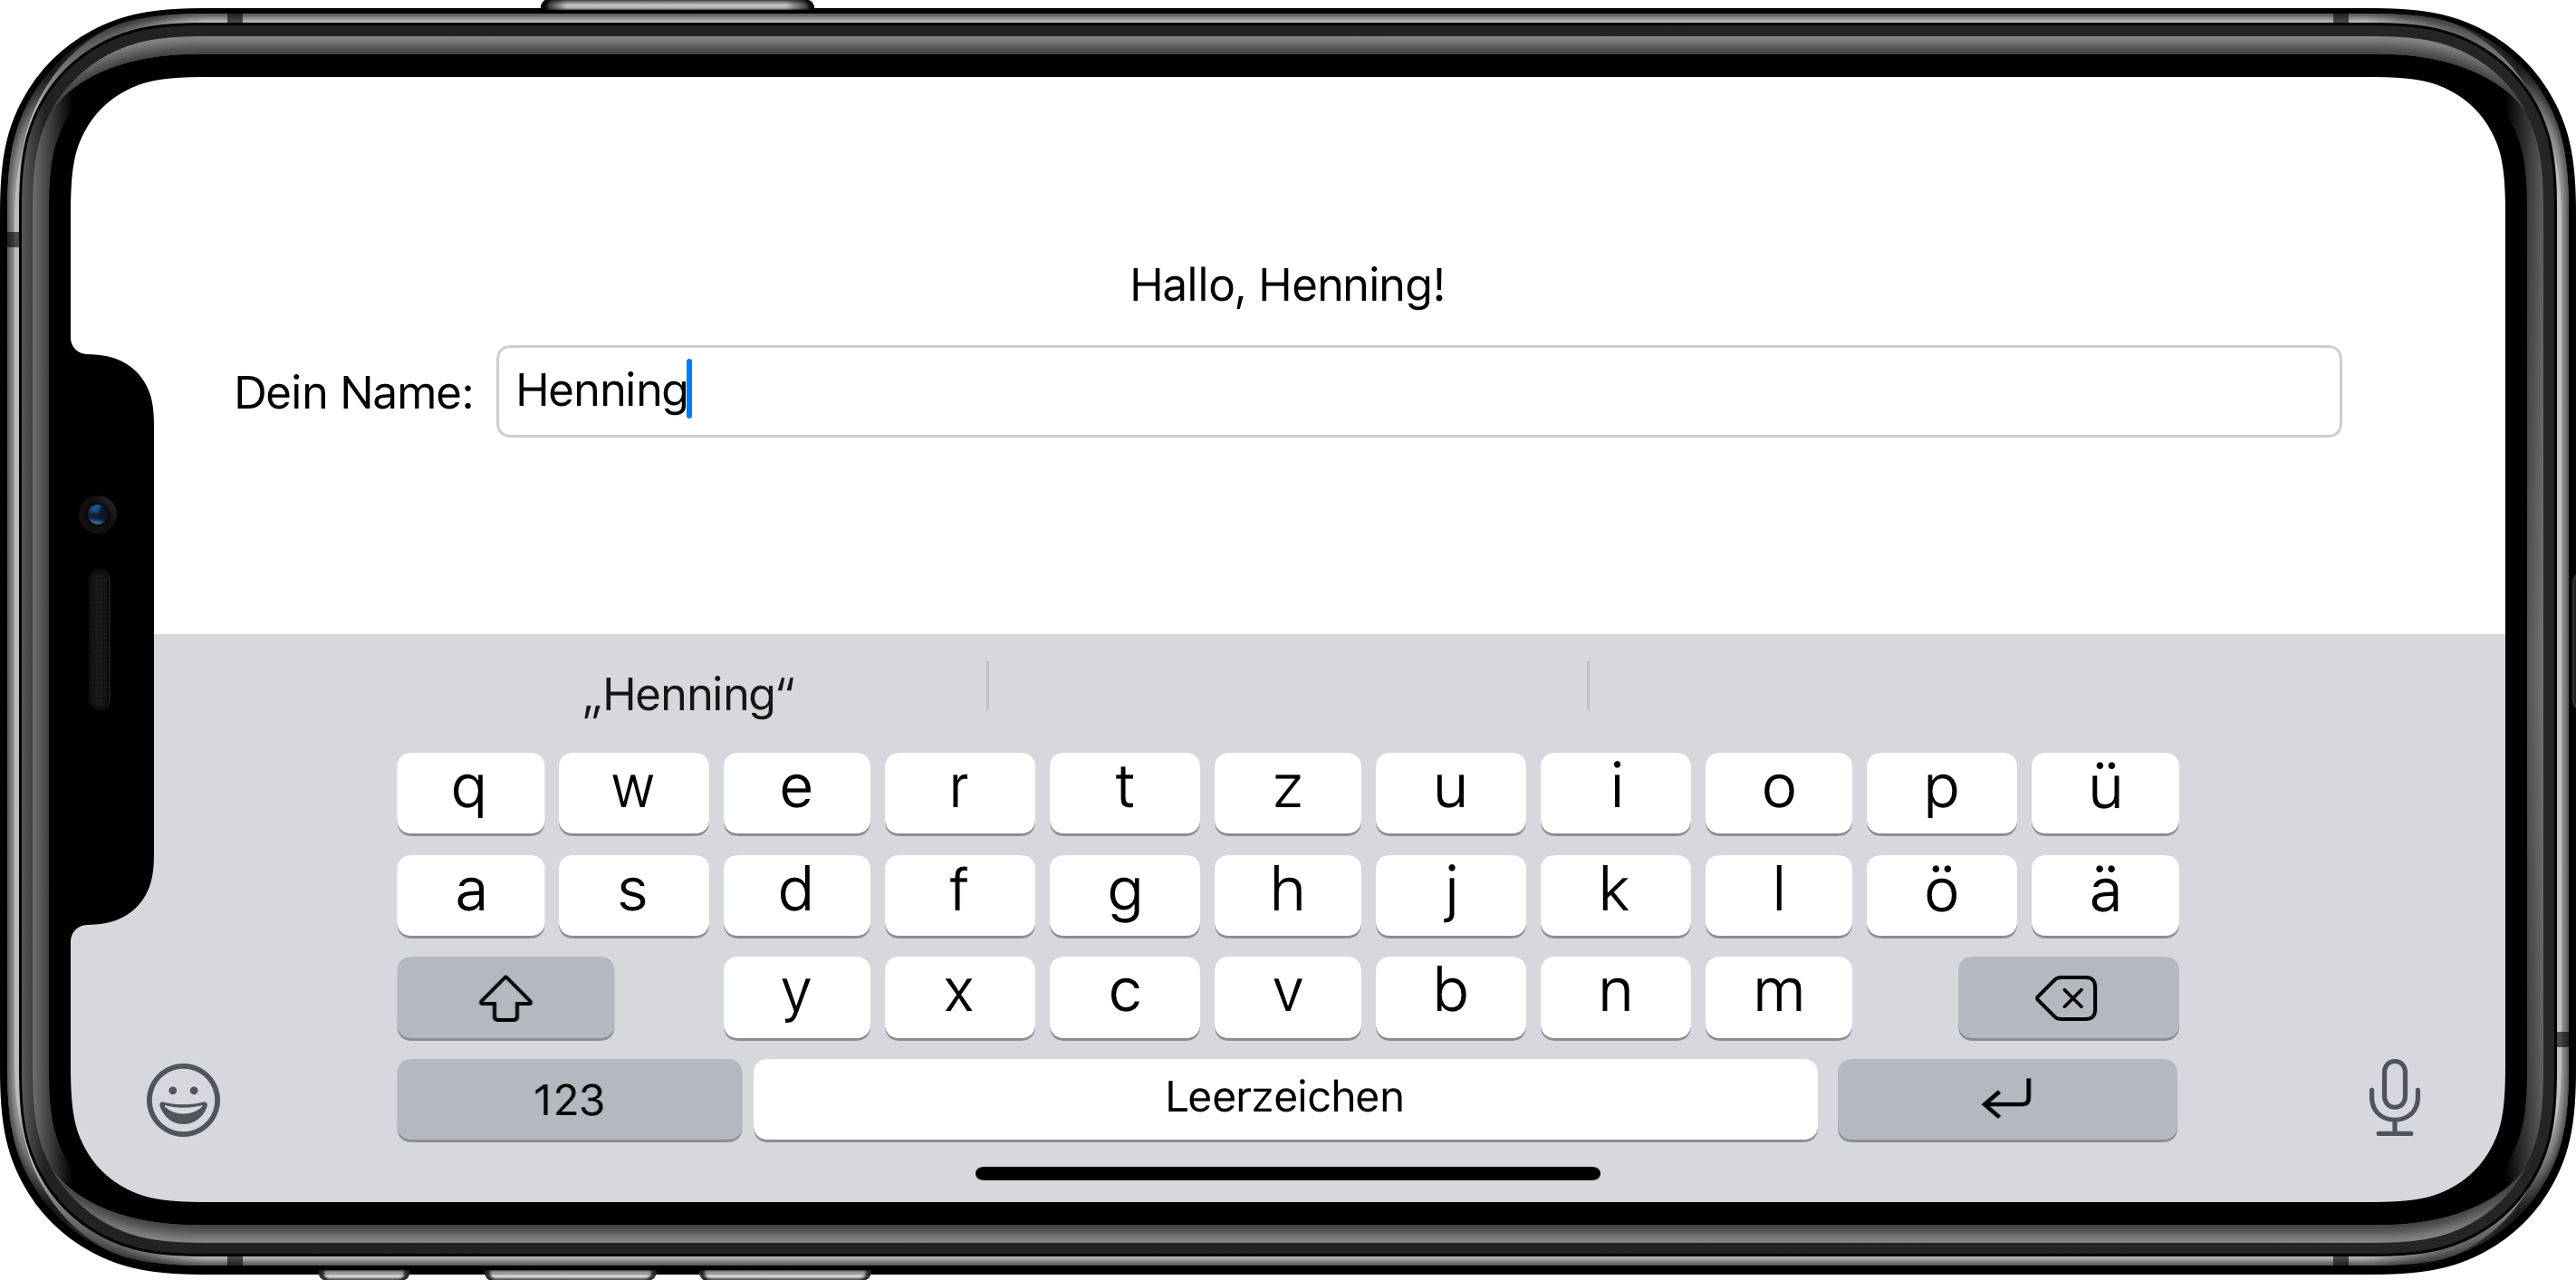
\includegraphics[width=.8\textwidth]{./images/methodology/swiftui/greeting_ui.png}
	\caption{\label{fig:ui:greeting}Einfache Oberfläche mit Label und Eingabefeld.}
\end{figure}

\subsubsection{Imperative Programmierung mit UIKit}

\begin{bsp}
Wir schauen uns zunächst an, wie wir dieses Ergebnis mithilfe imperativer Programmierung und UIKit realisieren können. Das \acl{UI} kann mit Xcode in einem Storyboard schnell realisiert werden, indem zwei \texttt{UILabel} und ein \texttt{UITextField} platziert werden. Für das obere \texttt{UILabel} wird nun ein Outlet \ref*{lst:uikit-greeting-outlet-label} und für das \texttt{UITextField} ein Outlet \ref*{lst:uikit-greeting-outlet-tf} und eine Action \ref*{lst:uikit-greeting-action-tf} in der zugehörigen \texttt{ViewController}-Klasse (\autoref{lst:uikit-greeting}) mit dem Storyboard verknüpft. Als Alternative zu Storyboards, können Oberflächen in Xcode auch mit Swift-Code aufgebaut werden. Diese Variante wollen wir hier nicht weiter verfolgen, da wir lediglich die Unterschiede zwischen imperativer und deklarativer Programmierung betrachten wollen.
	
\begin{lstlisting}[caption={\texttt{ViewController.swift}},label={lst:uikit-greeting}]
class ViewController: UIViewController {
    /*!\annotation{lst:uikit-greeting-outlet-label}!*/ @IBOutlet weak var label: UILabel!
    /*!\annotation{lst:uikit-greeting-outlet-tf}!*/ @IBOutlet weak var textField: UITextField!

    /*!\annotation{lst:uikit-greeting-action-tf}!*/ @IBAction func textFieldValueChanged(_ sender: Any) {
        guard let newText = textField.text else {
            return
        }
        label.text = "Hallo, \(newText)"
    }
}
\end{lstlisting}
\setcounter{lstannotation}{0}

Bei jeder Eingabe wird die Funktion \texttt{textFieldValueChanged(\_:)} aufgerufen. Hier wird zunächst geprüft, ob \texttt{textField.text} vom Typ \texttt{String?} ausgepackt werden kann, also nicht \texttt{nil} ist. Ist dies möglich, wird der Text des Labels neu gesetzt.

Möchte der Nutzer die Tastatur verschwinden lassen, muss dies über das \texttt{UI\-Text\-Field\-De\-le\-gate} separat implementiert werden. Bei einem Tap auf die Return-Taste passiert aktuell noch nichts.
\end{bsp}

\subsubsection{Deklarative Programmierung mit SwiftUI}

\begin{bsp}
Wie eine deklarative Programmierung mit SwiftUI \cite{Apple::SwiftUI-Documentation} aussehen kann, zeigt \autoref{lst:swiftui-greeting}. Ein \acl{UI}-Element in SwiftUI ist keine Klasse, sondern eine Struktur. Anders als Klassen, die in Swift Referenztypen sind, sind Strukturen Werttypen.

Zunächst deklarieren wir die Konformität zum \texttt{View}-Protokoll \ref*{lst:swiftui-greeting-struct}. Dieses Protokoll verlangt es, die Computed Property \texttt{body} \ref*{lst:swiftui-greeting-body} zu implementieren.

Unsere private Variable \texttt{name} \ref*{lst:swiftui-greeting-name} wird mit einem leeren \texttt{String} initialisiert. Die \texttt{@State}-Annotation ist ein sogenannter \doublequotes{Property Wrapper}. In \autoref{sec:swiftui:dependencies} wird genauer auf den Datenfluss durch SwiftUI eingegangen. Wichtig ist an dieser Stelle nur zu wissen, dass durch Manipulation einer mit \texttt{@State} annotierten Variable, die \texttt{body}-Property neu berechnet wird und dabei den geänderten Wert von \texttt{name} benutzt.

Das Keyword \texttt{some} \ref*{lst:swiftui-greeting-some} ist ein mit Swift 5.1 neu eingeführtes Feature der \doublequotes{Opaque Types}. Hier bedeutet es, dass der Rückgabe-Typ von \texttt{body} das Protokoll \texttt{View} implementieren muss. Uns ist dabei egal, von welchem Typ genau \texttt{body} ist. Es könnte sich um ein \texttt{Text}, ein \texttt{TextField} oder aber, wie hier, ein \texttt{VStack} \ref*{lst:swiftui-greeting-vstack} handeln.

Eine wichtige Sache, die man bei der Implementierung mit SwiftUI im Hinterkopf haben sollte, ist, dass für SwiftUI alles eine \texttt{View} ist und eine \texttt{View} auch nicht immer den gesamten Bildschirminhalt beschreibt. Eine \texttt{View} kann alles sein: Von der \texttt{NavigationView} mit Menüführung, über eine Liste (\texttt{List}) bis hin zum einfachen \texttt{Text}. Auch der \texttt{VStack} implementiert das \texttt{View}-Protokoll und erfüllt damit den Rückgabetyp von \texttt{some View}. Es sei angemerkt, dass das Schlüsselwort \texttt{return} in Swift optional ist, solange der Compiler erkennen kann, was zurückgegeben werden soll.

Innerhalb der geschweiften Klammern des \texttt{VStack} erwartet Swift nun weitere zu \texttt{View} konforme Elemente, die vertikal angeordnet werden sollen. Hier handelt es sich dabei um einen \texttt{Text} und einen \texttt{HStack}. Innerhalb des \texttt{String} \ref*{lst:swiftui-greeting-text} nutzen wir die \doublequotes{String-Interpolation}. Ausdrücke innerhalb der Zeichen \texttt{\textbackslash(...)} werden ausgewertet und in die Zeichenkette eingebaut.

Innerhalb des \texttt{HStack}, der Elemente horizontal anordnet, platzieren wir einen weiteren \texttt{Text} und ein \texttt{TextField} \ref*{lst:swiftui-greeting-textfield}. Der Konstruktor \texttt{init(\_:text:)} erwartet einen Platzhalter-Text und eine Variable für den Inhalt des Feldes vom generischen Typ \texttt{Binding<String>}. Der Typ \texttt{Binding<T>} wird ebenfalls genauer in \autoref{sec:swiftui:dependencies} vorgestellt. An dieser Stelle reicht es aus, das Dollar-Zeichen \$ als eine Art Referenz auf unsere private Variable \texttt{name} \ref*{lst:swiftui-greeting-name} zu sehen. Intern ist in Swift ein \texttt{String} als \texttt{struct} realisiert und damit ein Werttyp. SwiftUI löst auch das Problem der Bildschirmtastatur, indem es diese automatisch bei Antippen des Eingabefeldes anzeigt und mit Auswahl der Return-Taste verschwinden lässt.

Würden wir diesen Code ausführen, würde der \texttt{HStack} bis zum Rand des Displays ragen. Um einen Abstand um den \texttt{HStack} herum zu erreichen, rufen wir die Methode \texttt{padding(\_:)} \ref*{lst:swiftui-greeting-padding} des \texttt{HStack} auf. Diese Methode ist ein sogenannter \doublequotes{View Modifier}. Diese können auf Elemente, die das \texttt{View}-Protokoll implementieren, aufgerufen werden und verändern diese. Konkret geben \emph{View Modifier} wieder ein Element vom Typ \texttt{View} zurück. Hier ist das wieder ein \texttt{HStack}.

\begin{lstlisting}[caption={\texttt{GreetingView.swift}},label={lst:swiftui-greeting}]
struct GreetingView: /*!\annotation{lst:swiftui-greeting-struct}!*/ View {
    /*!\annotation{lst:swiftui-greeting-name}!*/ @State private var name: String = ""
    
    /*!\annotation{lst:swiftui-greeting-body}!*/ var body: /*!\annotation{lst:swiftui-greeting-some}!*/ some View {
        /*!\annotation{lst:swiftui-greeting-vstack}!*/ VStack {
            Text("Hallo, /*!\annotation{lst:swiftui-greeting-text}!*/ \(name)!")
            HStack {
                Text("Dein Name:")
                /*!\annotation{lst:swiftui-greeting-textfield}!*/ TextField("Name", text: $name)
            }
            /*!\annotation{lst:swiftui-greeting-padding}!*/ .padding()
        }
    }
}

\end{lstlisting}
\setcounter{lstannotation}{0}
	
\end{bsp}

\subsection{Vergleich zwischen imperativer und deklarativer Programmierung}

Der Ansatz der imperativen Programmierung ist es, auf Ereignisse zu reagieren und die Oberfläche dementsprechend anzupassen. Gibt der Nutzer im ersten Code-Beispiel (\autoref{lst:uikit-greeting}) einen Buchstaben ein, muss der Text des Labels manuell aktualisiert werden, indem wir den Wert des Eingabefeldes lesen und anschließend den Wert des Labels aktualisieren. Wir rufen also immer eine Funktion auf, wenn zum Beispiel auf eine Schaltfläche geklickt oder Text in ein Eingabefeld eingegeben wird.

Imperative Programmierung kann viele Probleme hervorrufen, von denen sich die meisten um den Zustand der Oberfläche drehen. Wir müssen verfolgen, in welchem Zustand sich unser Code befindet und sicherstellen, dass unsere Benutzeroberfläche diesen korrekt wiedergibt.

Angenommen, wir haben eine Oberfläche mit zwei Schaltern, die entweder \doublequotes{an} oder \doublequotes{aus} sein können. Jeder Schalter verändert eine boolesche Variable, die sich auf die Oberfläche auswirkt. Bei zwei Booleans, \texttt{a} und \texttt{b}, haben wir insgesamt vier Zustände:

\begin{table}[H]
	\centering
\begin{tabular}{rl}
	\thead{\texttt{a}} & \thead{\texttt{b}}\\
	\midrule
	\texttt{true} & \texttt{true}\\
	\texttt{true} & \texttt{false}\\
	\texttt{false} & \texttt{true}\\
	\texttt{false} & \texttt{false}\\
\end{tabular}
\caption{Vier Zustände bei zwei Booleans.}
\end{table}

Bei zwei Booleans mag dies vielleicht noch überschaubar wirken. Handelt es sich allerdings um noch mehr oder gar andere Werte, wie Strings oder Integer-Zahlen, werden die Zustände deutlich komplexer. Eine imperative Programmierung der Benutzeroberfläche bedeutet es, zu beschreiben, \textbf{wie} die Oberfläche auf Zustandsänderungen reagieren soll.

Im Gegensatz dazu, wird bei der deklarativen Programmierung beschrieben, \textbf{was} die Oberfläche leisten soll. SwiftUI erlaubt es uns, das System über alle möglichen Zustände unserer App auf einmal zu informieren.

Wir könnten zum Beispiel festlegen, dass, wenn der Benutzer eingeloggt ist, eine Begrüßungsnachricht angezeigt wird, aber wenn er ausgeloggt ist, eine Login-Schaltfläche angezeigt wird. Wir müssen keinen Code schreiben, um uns von Hand zwischen diesen beiden Zuständen zu bewegen. Stattdessen lassen wir SwiftUI zwischen den verschiedenen Benutzeroberflächen hin und her wechseln, wenn sich der Zustand ändert. Wir legen nur fest, was angezeigt werden soll, abhängig davon, ob der Benutzer an- oder abgemeldet ist. Wenn wir also den Status der Authentifizierung ändern, aktualisiert SwiftUI die Benutzeroberfläche für uns.

Das ist es, was deklarativ bedeutet: Wir modifizieren die Benutzeroberfläche nicht von Hand. Wir definieren nur Regeln, die unser System befolgen soll, und überlassen es SwiftUI, dafür zu sorgen, wie diese Regeln umgesetzt werden.

\subsection{Weitere Vorteile durch SwiftUI}

SwiftUI bringt darüberhinaus auch noch weitere Vorteile mit sich. Der Code, den wir schreiben, ist plattformunabhängig. Oben stehender Code kann ohne Veränderung $ 1:1 $ in einem watchOS-Projekt verwendet werden. \autoref{fig:ui:watch} zeigt, wie die Benutzeroberfläche des Codes aus \autoref{lst:swiftui-greeting} auf einer Apple Watch aussieht.

\begin{figure}
	\centering
	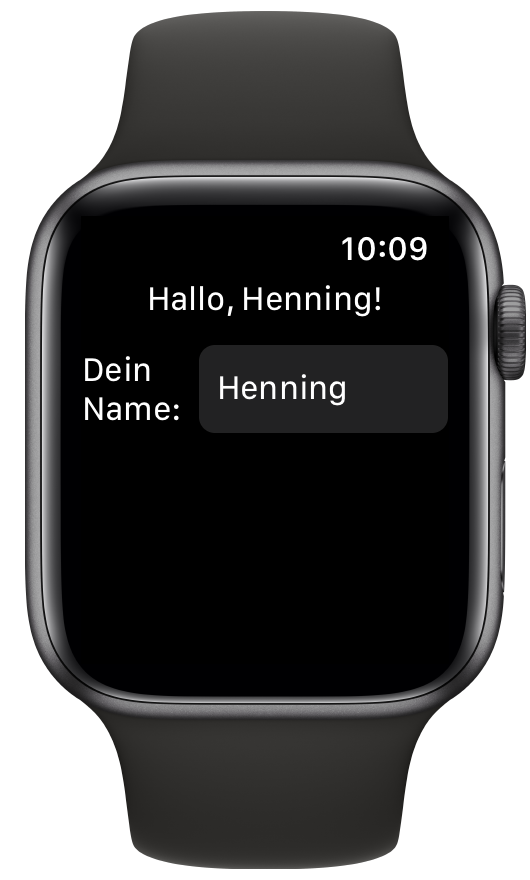
\includegraphics[width=.3\textwidth]{./images/methodology/swiftui/watch.png}
	\caption{\label{fig:ui:watch}Die Oberfläche auf der Apple Watch.}
\end{figure}

Ebenso unterstützt SwiftUI die Lokalisierung der Anwendung. Weiter oben wurde erwähnt, dass ein \texttt{Text}-Element einen \texttt{String} erwartet. Intern wandelt Swift diesen \texttt{String} in einen \texttt{LocalizedStringKey} um und übergibt diesen an die \texttt{Text}-Komponente. Initialisieren wir das \texttt{Text}-Element hingegen direkt mit einem \texttt{LocalizedStringKey}, substituiert Swift diesen durch die entsprechende Übersetzung. \autoref{lst:swiftui-greeting-loc} zeigt, wie der Swift-Code hierfür aussehen muss. \autoref{bsp:ui:en} und \autoref{bsp:ui:fr} zeigen die Oberfläche auf Englisch und Französisch mit den zugehörigen Übersetzungs-Dateien.

\begin{lstlisting}[caption={\texttt{GreetingViewLocalized.swift}},label={lst:swiftui-greeting-loc}]
struct GreetingViewLocalized: View {
    @State private var name: String = ""

    var body: some View {
        VStack {
            Text("user.greeting \(name)")
            HStack {
                Text("user.enter")
                TextField("user.name.placeholder", text: $name)
            }
            .padding()
        }
    }
}
\end{lstlisting}\setcounter{lstannotation}{0}

\begin{figure}[ht]
\begin{minipage}{0.5\textwidth}
\begin{lstlisting}[title={\texttt{Localizable.strings (English)}},label={lst:swiftui-greeting-en}]
"user.greeting %@" = "Hello, %@!";
"user.enter" = "Your name:";
"user.name.placeholder" = "Name";
\end{lstlisting}\setcounter{lstannotation}{0}
\begin{figure}[H]
\centering
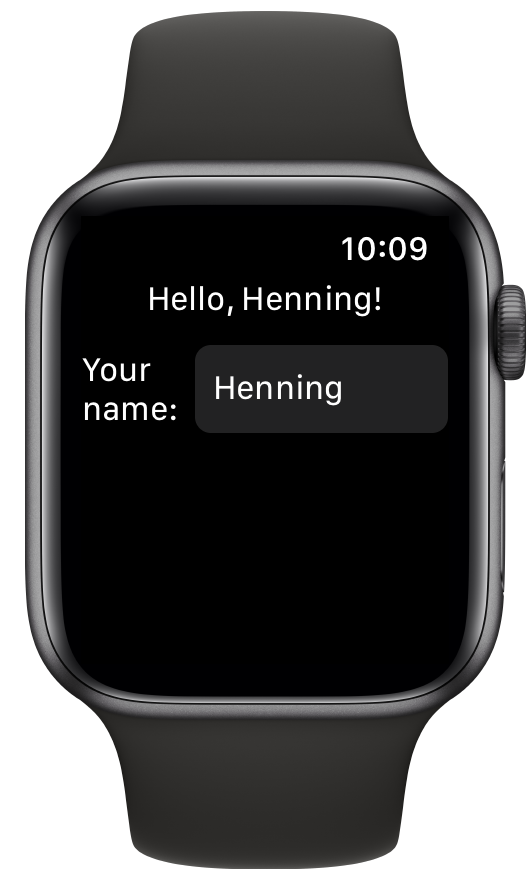
\includegraphics[width=.6\textwidth]{./images/methodology/swiftui/watch-en.png}
\caption{\label{bsp:ui:en}Das englische Interface.}
\end{figure}
\end{minipage}
\begin{minipage}{0.5\textwidth}
\begin{lstlisting}[title={\texttt{Localizable.strings (French)}},label={lst:swiftui-greeting-fr},language=Swift]
"user.greeting %@" = "Salut, %@!";
"user.enter" = "Ton nom:";
"user.name.placeholder" = "Nom";
\end{lstlisting}\setcounter{lstannotation}{0}
\begin{figure}[H]
\centering
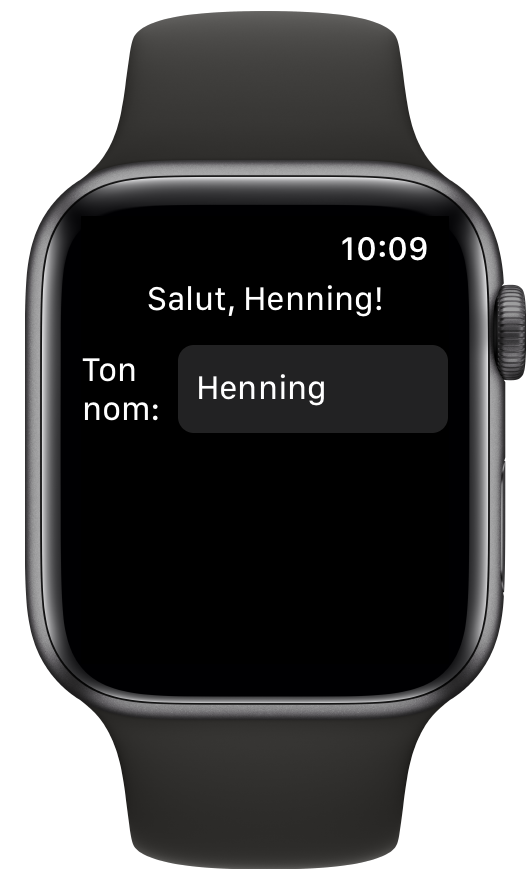
\includegraphics[width=.6\textwidth]{./images/methodology/swiftui/watch-fr.png}
\caption{\label{bsp:ui:fr}Das französische Interface.}
\end{figure}
\end{minipage}
\end{figure}

Doch hier enden die Möglichkeiten mit SwiftUI noch nicht. Zusätzlich bringt das Framework weitere Funktionalitäten, wie etwa eine Unterstützung des \emph{Dark Modes}, automatische Anpassungen der Schriftgröße nach Wünschen des Nutzers oder die Sprachausgabe für Menschen mit Sehbeeinträchtigungen durch \emph{VoiceOver}, mit sich.

\subsection{Abhängigkeiten}\label{sec:swiftui:dependencies}

Wir haben bereits den \emph{Property Wrapper} \texttt{@State} kennengelernt. Eine mit \texttt{@State} annotierte Variable ist eine \doublequotes{Source of Truth}\footnote{Dieses Wort ist sehr schnell zu einem Buzzword der WWDC 2019 geworden, auf der Apple SwiftUI vorgestellt hat.} (dt. \doublequotes{Quelle der Wahrheit}) \cite{Apple::SwiftUI-Documentation}.

\subsubsection{\doublequotes{Sources of Truth} und \doublequotes{Derived Values}}

Im Kontext der Programmierung von Benutzerschnittstellen bedeutet dies, dass wir auf redundante Speicherung von Informationen verzichten sollen. In \autoref{lst:swiftui-greeting} deklarieren wir unsere Variable \texttt{name} mit \texttt{@State} als \emph{Source of Truth}. In diesem Kontext erschließt sich die Redundanz noch nicht sofort. Wenn wir uns allerdings eine umfangreichere App vorstellen, kann es sein, dass wir an mehreren Stellen den Namen des Nutzers anzeigen oder auch verändern wollen. Würden wir in jeder einzelnen \texttt{View} eine eigene Variable \texttt{name} definieren, müssten wir auch dafür sorgen, alle Variablen aktuell zu halten. Als Werttyp kann eine \texttt{View} nämlich keine Referenzen auf lokale Variablen bereitstellen.

Eine weitere Funktion des \texttt{State} ist der, dass SwiftUI sich um die Speicherung und \doublequotes{Überwachung} aller Variablen kümmert, die als Zustand deklariert werden. Wenn sich der Wert ändert, verliert eine \texttt{View} ihre Gültigkeit und berechnet den \texttt{body} neu.

Um einen \texttt{State} an eine andere \texttt{View} in der Hierarchie zu übergeben, muss der Variablenname mit vorangestelltem \$-Zeichen verwendet werden. Dadurch wird eine Bindung auf den \texttt{State} abgerufen. In der aufgerufenen \texttt{View} wird dann die Variable nicht mit \texttt{@State} deklariert. Hier wird \texttt{@Binding} genutzt. Eine Bindung ist keine \emph{Source of Truth}, sondern ein \doublequotes{Derived Value} (dt. \doublequotes{Abgeleiteter Wert}).

Auch \texttt{@Binding} sogt für eine Aktualisierung der \texttt{View}, sobald sich der Wert des referenzierten \texttt{State}, also der \emph{Source of Truth}, ändert. Intern sorgt Swift dafür, dass alle annotierten Variablen auf die gleiche Speicherzelle auf dem Stack zeigen. In \autoref{lst:swiftui-greeting} erwartet das Eingabefeld eine Bindung auf den \texttt{State}, die wir durch das \$-Zeichen bekommen.

\subsubsection{Binden von Klassen durch \doublequotes{ObservableObjects}}

Angenommen, wir haben eine eigene Klasse, die sich um das Modell der App kümmert. \texttt{@State} können wir in der Wurzel der View-Hierarchie nicht verwenden, um eine \emph{Source of Truth} unseres Modells zu deklarieren. Hierfür nutzen wir das von SwiftUI bereitgestellte Protokoll des \texttt{ObservableObject}.

Unser Modell in \autoref{lst:swiftui-model} implementiert dieses Protokoll \ref*{lst:swiftui-model-protocol}. Hierdurch erhält die Klasse die Variable \texttt{objectWillChange}, einen \emph{Publisher}. Ein \emph{Publisher} wird dazu genutzt, Bindungen für die \texttt{Views} bereitzustellen. Sobald eine Variable des Modells verändert wird \ref*{lst:swiftui-model-willset}, muss die Funktion \texttt{send()} \ref*{lst:swiftui-model-send} unseres \emph{Publishers} \texttt{objectWillChange} aufgerufen werden. Anschließend können wir den neuen Wert (Zugriff innerhalb des \texttt{willSet}-Blocks über \texttt{newValue}) beispielsweise auf ein Server-Backend hochladen, um die Daten zu persistieren.

Anstatt für jede einzelne Variable manuell \texttt{send()} aufzurufen, stellt Swift die \texttt{@Published}-Annotation \ref*{lst:swiftui-model-published} zur Verfügung. Diese sorgt dafür, dass automatisch vor jedem Setzen der Variable, die Funktion \texttt{send()} des \emph{Publishers} aufgerufen wird.

\begin{lstlisting}[caption={Model.swift},label={lst:swiftui-model}]
final class Model: /*!\annotation{lst:swiftui-model-protocol}!*/ ObservableObject  {
    var age: Int = 0 {
        /*!\annotation{lst:swiftui-model-willset}!*/ willSet {
            /*!\annotation{lst:swiftui-model-send}!*/ objectWillChange.send()
            // Neuen Wert z. B. auf Server-Backend abspeichern.
        }
    }
    /*!\annotation{lst:swiftui-model-published}!*/ @Published var name: String = "" /* {
        willSet {
            // objectWillChange.send() wird automatisch aufgerufen.
            // Neuen Wert z. B. auf Server-Backend abspeichern.
        }
    } */
}
\end{lstlisting}\setcounter{lstannotation}{0}

Innerhalb einer \texttt{View} (\autoref{lst:swiftui-model-view}) haben wir zwei Möglichkeiten, auf die Nachrichten eines \emph{Publishers} zu reagieren. Wir können unser Modell entweder mit \texttt{@ObservedObject} \ref*{lst:swiftui-model-obs}\ref*{lst:swiftui-model-obs2} oder \texttt{@EnvironmentObject} \ref*{lst:swiftui-model-env} annotieren. Anschließend kann das Modell in der \texttt{View} verwendet werden \ref*{lst:swiftui-model-usage}. 

Im Beispiel wurden noch keine Instanzen\footnote{Es sei angemerkt, dass im Beispiel nicht dafür gesorgt wird, beide Modelle synchron zu halten. Es würden zwei Instanzen und damit zwei \emph{Sources of Truth} des Modells auf dem Stack existieren. Es sollte selbstverständlich nur eine einzige Instanz existieren.} des Modells erzeugt. Für ein \texttt{ObservedObject} muss dieses entweder in der \texttt{ModelView} initialisiert \ref*{lst:swiftui-model-obs2} oder beim Aufruf des Konstruktors der \texttt{ModelView} übergeben werden \ref*{lst:swiftui-model-obs}. Dies geschieht in der aufrufenden \texttt{ParentView} über \texttt{ModelView(model: Model())}. Möchte unsere \texttt{ModelView} das Objekt an eine untergeordnete \texttt{View} übergeben, geschieht das ebenfalls über den Konstruktor \texttt{SubView(model: modelObs)} \ref*{lst:swiftui-model-sub}. Alternativ kann auch direkt ein Bindung mit beispielsweise \texttt{\$modelObs.name} an die untergeordnete \texttt{View} übergeben werden

 Bei der Übergabe eines Modells an andere \texttt{Views} kann es bei einer großen \texttt{View}-Hierarchie schnell unübersichtlich werden. Abhilfe schafft \texttt{@EnvironmentObject} \ref*{lst:swiftui-model-env}. Hierzu wird die Instanz des Modells an eine Wurzel-\texttt{View} mit  \texttt{RootView().environmentObject(Model())} übergeben. Dies passiert bei einem neuen Xcode-Projekt üblicherweise im \texttt{SceneDelegate}. Alle dieser Wurzel untergeordneten \texttt{Views} können nun mit \texttt{@EnvironmentObject} auf diese Instanz automatisch zugreifen. Swift kümmert sich darum, das Modell zur Verfügung zu stellen und einzubinden.

\begin{lstlisting}[caption={ModelView.swift},label={lst:swiftui-model-view}]
struct ModelView: View {
    /*!\annotation{lst:swiftui-model-obs}!*/ @ObservedObject var modelObs: Model
    // Oder bei Initialisierung innerhalb der View:
    // /*!\annotation{lst:swiftui-model-obs2}!*/ @ObservedObject var modelObs: Model = Model()
    /*!\annotation{lst:swiftui-model-env}!*/ @EnvironmentObject var modelEnv: Model
    
    var body: some View {
        VStack {
            /*!\annotation{lst:swiftui-model-usage}!*/ Text("\(modelObs.name) ist \(modelEnv.age) Jahre alt.")
            /*!\annotation{lst:swiftui-model-sub}!*/ SubView(model: modelObs)
        }
    }
}
\end{lstlisting}\setcounter{lstannotation}{0}

Es gibt keine Regel, wann ein \texttt{State}, ein \texttt{ObservedObject} oder ein \texttt{EnvironmentObject} zu verwenden sind. Dies kann nur für den jeweiligen Einsatzzweck entschieden werden. \texttt{States} sind dann zu empfehlen, wenn die jeweilige \texttt{View} alleinigen Zugriff benötigt. Bei multiplen Zugriffen sollte ein \texttt{ObservableObject} verwendet werden, abhängig davon, wie groß die \texttt{View}-Hierarchie ist und an welchen Stellen die Daten benötigt werden. \autoref{tab:data-flow} zeigt noch einmal alle möglichen Wege des Datenflusses mit SwiftUI auf.

\begin{table}[H]
\centering
\begin{tabular}{c|cc}
& \emph{Source of Truth} & \emph{Derived Value}\\
\hline&&\\
Read-only & Konstante & Property\\&&\\
Read-write & \makecell{\texttt{@State}\\\texttt{ObservableObject}} & \makecell{\texttt{@Binding}\\\texttt{@ObservedObject}\\\texttt{@EnvironmentObject}}\\
\end{tabular}
\caption{\label{tab:data-flow}Übersicht über die verschiedenen Datenfluss-Arten in SwiftUI.}
\end{table}

\section{Bluetooth Low Energy mit CoreBluetooth}\label{sec:bluetooth}

Für die drahtlose Kommunikation mit  Bluetooth existieren mehrere Arten. Die bekanntesten sind \doublequotes{Bluetooth Classic}, \doublequotes{\acl{BLE}} und \doublequotes{iBeacon}.

\subsection{Bluetooth Classic, Bluetooth Low Energy und iBeacon}

\acl{BT Classic} und \acl{BLE} sind von der \doublequotes{Bluetooth Special Interest Group} herausgegebene Standards zur drahtlosen Kommunikation zwischen Geräten \cite{Group:2019:Bluetooth-Core-Specification}. Der ursprüngliche Standard, \ac{BT Classic}, der früher nur \doublequotes{Bluetooth} genannt wurde, kann beispielsweise genutzt werden, um Dateien zwischen Geräten zu übertragen oder drahtlose Kopfhörer mit einem Gerät zu verbinden. Ein großer Nachteil von \ac{BT Classic} ist allerdings der hohe Stromverbrauch. Gerade für Geräte, die nur gelegentlich Daten kleiner Größe austauschen, braucht es keine permanente Verbindung, die in der Lage ist, Audiosignale zu übertragen. 

Mit \ac{BLE} existiert ein weiterer Standard, der -- wie der Name schon sagt -- sehr stromsparend ist. Er wurde mit der \emph{Bluetooth Core Specification 4.0} eingeführt. Der Standard basiert auf einer Client-Server-Architektur. Clients werden als \doublequotes{Centrals} bezeichnet. \emph{Centrals} versuchen, auf die Daten der Peripheriegeräte (\emph{Peripherals}), den Servern, zuzugreifen. Peripheriegeräte stellen die Eigenschaften (\emph{Characteristics}) durch Werte dar. Zusammengehörige Eigenschaften werden in einem übergeordneten Konstrukt zusammengefasst, das als \emph{Service} bezeichnet wird. Eine Eigenschaft besitzt keinen oder mehrere Deskriptoren (\emph{Descriptors}). Diese können verschiedene Arten von Metadaten enthalten, mit denen sie die verknüpfte Charakteristik ergänzen können. Mithilfe des \ac{CCCD} können beispielsweise die Benachrichtigungen durch die Peripheriegeräte empfangen werden. \autoref{dia:ble} veranschaulicht den Zusammenhang der einzelnen Komponenten.

Jeder \emph{Service}, jede \emph{Charakteristic} und jeder \emph{Descriptor} muss durch einen eindeutigen Bezeichner, einen \ac{UUID}, identifiziert werden können. \acp{UUID} können 16- oder 128-Bit-Werte sein und zum Beispiel mit \texttt{uuidgen} in einer Bash generiert werden.

Zudem ist es möglich, \ac{BLE}-Geräte ad-hoc miteinander zu verbinden, ohne vorher eine explizite Verbindung (\emph{Pairing}) zu initiieren. Ein explizites \emph{Pairing} ist nur für verschlüsselte Übertragungen notwendig.

\begin{figure}[ht]
	\begin{adjustbox}{scale=0.7,center} % 	\begin{adjustbox}{scale=0.7,center}
		\begin{tikzpicture}
		\tikzstyle{all} = [draw, ultra thick, align=left]
		\tikzstyle{block} = [rectangle, all, inner sep=1em, rounded corners=5pt]
		\node[block, fill=cyan!20] {
			Server\\[1em]
			\tikz \node[block, fill=magenta!20] {
				Service\\{\ttfamily UUID}\\[1em]
				\tikz \node[block, fill=yellow!20] {
					Characteristic\\{\ttfamily UUID}\\{\ttfamily Value}\\[1em]
					\tikz \node[block, fill=green!20] {
						Descriptor\\{\ttfamily UUID}\\{\ttfamily Value}\\[1em]$0..*$
					};\\[1em]$1..*$
				};\\[1em]$1..*$
			};\\
		};
		\end{tikzpicture}
	\end{adjustbox}
	\caption{\label{dia:ble}Aufbau eines BLE-Peripheriegeräts. Nach \cite{Kolban:2018:BLE-C-Guide}}
\end{figure}

iBeacon ist ein von Apple eingeführter Standard, der auf \ac{BLE} aufbaut, der zur Lokalisierung von Geräten genutzt wird \cite{Apple-Inc.::iBeacon}\cite{Hiramatsu:2017:Outdoor-Studying-System}. Ein iBeacon kann keine Daten empfangen, speichern oder Benachrichtigungen senden. Gesendet werden nur die eigene \ac{UUID}, sowie die Werte \emph{Major} und \emph{Minor}, beide vorzeichenlose Integer zwischen 0 und 65535.

\subsection{Core Bluetooth}

Für die Bluetooth-Kommunikation stellt Apple das \doublequotes{\acl{CB}}-Framework (\acs{CB}) bereit \cite{Apple-Inc.::Core-Bluetooth}. Dieses Framework bietet Unterstützung für \ac{BT Classic} und \ac{BLE}. iBeacon ist Bestandteil des \doublequotes{Core Location}-Frameworks, da es von Apple nur für die Positionsbestimmung vorgesehen ist. Die iBeacon-Technologie wird in dieser Arbeit nicht weiter verfolgt.

Das \ac{CB}-Framework unterstützt für \ac{BLE} grundsätzlich beide Betriebsmodi\footnote{Der Xcode Simulator unterstützt seit iOS 7 kein \acl{CB} mehr. Zum Testen, wird ein physisches Gerät benötigt.}. Ein iOS-Gerät kann sowohl als Client (\emph{Central}), als auch als Server (\emph{Peripheral}) agieren und Verbindungen auch im Hintergrund nutzen. Bei einer Implementierung ist es wichtig zu wissen, dass iOS-Geräte, die im Hintergrund einen \emph{Service} bereitstellen, nur von anderen iOS-Geräten gefunden werden können und auch nur, wenn diese explizit nach den \emph{Service}-\acp{UUID} suchen\footnote{\url{https://developer.apple.com/library/archive/documentation/NetworkingInternetWeb/Conceptual/CoreBluetooth_concepts/CoreBluetoothBackgroundProcessingForIOSApps/PerformingTasksWhileYourAppIsInTheBackground.html\#//apple_ref/doc/uid/TP40013257-CH7-SW9}}!

Bei der Apple Watch sind die Funktionalitäten deutlich eingeschränkter. Mit Bluetooth als wichtigste Kommunikationsschnittstelle, steht \acl{CB} unter watchOS nur eingeschränkt zur Verfügung, um sicherzustellen, dass alle Systemaktivitäten ausgeführt werden können. Die Apple Watch kann nur als \emph{Central} agieren und höchstens zwei Peripheriegeräte gleichzeitig verwenden. Verbindungen zu \emph{Peripherals} werden zudem getrennt, sobald die App angehalten wird.

\section{Speicherung von Daten in der iCloud}

Mit der iCloud hat Apple eine einfache Möglichkeit geschaffen, Cloud-Backups von Geräten zu erstellen und Dateien beziehungsweise Daten zwischen verschiedenen Geräten zu synchronisieren. Es gibt drei Arten, die iCloud in einer App zu verwenden: als Schlüssel-Wert-Paare (\emph{Key-Value}-Speicher), in einer Art Datenbank (\emph{CloudKit}) oder auf Dateiebene (\emph{iCloud Drive}).

Wir wollen hier nur die erste Variante betrachten. \emph{CloudKit} ist für eine kleine Anwendung, wie wir sie schreiben, viel zu mächtig. Einen datenbankähnlichen Speicher benötigen wir für die Speicherung einzelner Attribute nicht. Da \emph{iCloud Drive} hauptsächlich für dokumentenbasierte Anwendungen, wie etwa Apples eigene Office-Lösungen \emph{Pages}, \emph{Numbers} und \emph{Keynote}, interessant ist, wollen wir uns nur der ersten Variante widmen.

\subsection{Key-Value Speicher}

Diese Art der Synchronisation ist dazu gedacht, kleine Daten zwischen den Geräten auszutauschen. Maximal können im \emph{Key-Value}-Speicher der iCloud 1024 Einträge gespeichert werden, der insgesamt nicht größer als \SI{1}{\mega\byte} sein darf. Die Länge eines Schlüssels ist auf  \SI{64}{\byte} begrenzt \cite{Kofler:2019:Swift-5---Das-umfassende-Handbuch}. Leider unterstützt watchOS diese iCloud-Variante nicht. \autoref{sec:user-defaults} zeigt, wie Daten lokal auf der Apple Watch gespeichert werden können und in \autoref{sec:watch-connectivity} wird die Kommunikation zwischen iPhone und Apple Watch vorgestellt.

Die Klasse \texttt{NSUbiquitousKeyValueStore} ist Bestandteil des \texttt{Foundation}-Frameworks, welches die grundlegendste Bibliothek von Swift ist. Nach Aktivierung \emph{Key-Value-Capability} in Xcode und Erzeugen der Instanz \ref*{lst:cloud-init} in \autoref{lst:cloud-kv}, kann der Speicher ganz leicht verwendet werden.

Um einen Wert zu speichern, wird die Methode \texttt{set(\_:forKey:)} \ref*{lst:cloud-set} genutzt. Diese ist mehrfach vorhanden und akzeptiert viele Datentypen, wie etwa \texttt{String}, \texttt{Data} oder auch \texttt{Any}.

Gelesen wird ein Wert mit Aufruf der Methode, die dem erwarteten Typ entspricht. Um einen \texttt{String} zu lesen, wird die Methode \texttt{string(forKey:)} \ref*{lst:cloud-get} verwendet. Die Methode \texttt{object(forKey:)} gibt uns beispielsweise ein Objekt vom Typ \texttt{Any?} zurück. Viele Methoden, die zum Lesen von Werten gedacht sind, geben uns ein \texttt{Optional} dieses Typs wieder, da nicht für jeden Schlüssel ein Wert ermittelt werden kann.

\begin{lstlisting}[caption={Storage.swift},label={lst:cloud-kv}]
final class Storage {
    /*!\annotation{lst:cloud-init}!*/ static let kvStore = NSUbiquitousKeyValueStore()
    
    func setString(key: String, value: String) {
        /*!\annotation{lst:cloud-set}!*/ kvStore.set(value, forKey: key)
    }
    
    func getString(key: String) -> String? {
        /*!\annotation{lst:cloud-get}!*/ kvStore.string(forKey: key)
    }
}
\end{lstlisting}\setcounter{lstannotation}{0}

Bei Verwendung dieses Speichers, behält das Gerät eine lokale Kopie der Daten. Nicht immer ist eine Verbindung mit dem Internet und damit der iCloud vorhanden. Um die Synchronisation der beiden Kopien kümmert sich das Betriebssystem. Ein Aufruf der \texttt{synchronize()}-Methode erzwingt dies, wenn es möglich ist.

\subsection{Lokale Alternative mit User-Defaults}\label{sec:user-defaults}

Um Schlüssel-Wert-Paare nur lokal zu speichern eignen sich auch die \emph{User-Defaults}. Falls keine geräteübergreifende Synchronisation gewünscht ist, können statt des \texttt{NS\-Ubiq\-ui\-tous\-Key\-Value\-Store} die \emph{User-Defaults} verwendet werden. Ersetzt man in \autoref{lst:cloud-kv} \doublequotes{\texttt{NS\-Ubiq\-ui\-tous\-Key\-Value\-Store()}} \ref*{lst:cloud-init} durch \doublequotes{\texttt{UserDefaults.standard}}, hat man eine Lösung, die Daten lokal persistiert. Diese Variante steht unter watchOS zur Verfügung.

\section{Kommunikation zwischen iPhone und Apple Watch}\label{sec:watch-connectivity}

Für die Kommunikation zwischen iPhone und Apple Watch existiert das \emph{WatchConnectivity}-Framework. Nach Herstellen der Session beim Start der Apps, können Nachrichten auf mehrere Arten gesendet werden. Neben dem Transfer von Dateien und Information für \emph{Komplikationen} des \emph{Watchfaces}, gibt es drei Methoden, die einfache Nachrichten verschicken. Diese akzeptieren jeweils ein \emph{Dictionary} vom Typ \texttt{[String: Any]}.

Die einfachste Art wird mit \texttt{WC\-Session.default.send\-Message(\_:reply\-Handler:error\-Handler:)} verschickt. Diese Methode verschickt die Nachricht nur, wenn die App auf beiden Geräten im Vordergrund läuft. Dann ist der \texttt{activation\-State} der Session gleich \texttt{WC\-Session\-Activation\-State.activated}. Wurde die Nachricht übertragen, wird der \texttt{reply\-Handler} aufgerufen, bei Fehlern der \texttt{error\-Handler}.

Möchte man Nachrichten an die geschlossene \emph{Counterpart}-App übertragen, kann man die Methoden \texttt{updateApplicationContext(\_:)} und \texttt{transfer\-User\-Info(\_:)} der Session verwenden. Beide senden das \emph{Dictionary} an das andere Gerät, das die Nachricht zwischenspeichert. Sobald die Anwendung auf diesem Gerät geöffnet wird, wird die Nachricht ausgeliefert. Der Unterschied zwischen einem \emph{Application\-Context} und einer \emph{User\-Info} ist folgender: Existiert auf dem anderen Gerät bereits ein nicht-ausgelieferter \emph{Application\-Context}, wird bei Empfang eines weiteren Kontexts der Wartende überschrieben. Auf diese Weise kann zum Beispiel ein Zustand der App übertragen werden, wenn wir nur an der letzten Version interessiert sind. Bei einem Chat wollen wir beispielsweise allerdings, dass das andere Gerät alle empfangenen Chat-Mitteilungen bekommt. Hierzu eignet sich die \emph{User\-Info}: Alle empfangenen \emph{User\-Infos} werden in einer FIFO-Queue gespeichert und bei Öffnen der App in Empfangsreihenfolge übergeben. So geht keine Nachricht verloren.

  	\chapter{Realisierung eines Prototyps}

Für das Projekt \doublequotes{UrbanLife+} soll nun ein Prototyp einer mobilen Anwendung realisiert werden. An der Universität Leipzig wird bereits eine mobile Anwendung mit Google's Development Kit \emph{Flutter} entwickelt. Dieses dient dazu, plattformübergreifende Anwendungen für beispielsweise iOS und Android zu programmieren. Um eine App für die Apple Watch zu programmieren, existieren jedoch keine Tools. Soll eine Anwendung auf der Apple Watch laufen, muss auf Apple's eigene Programmiersprache \emph{Swift} zurückgegriffen werden.

Wir wollen ein \doublequotes{Human-centred Design} für unsere App erreichen und folgen somit der Norm ISO 9241-210 (vgl. \autoref{dia:human-centered-design-process}). Der Code der App lässt sich unter \url{https://github.com/hhontheim/UrbanLifePlusApp} herunterladen.

\section{Beschreiben des Nutzungskontexts}

Um den Nutzungskontext zu verstehen, verschaffen wir uns zunächst einen Überblick über das Projekt.

Das Ziel des Projekts ist es, die Teilhabe von Senioren im öffentlichen Raum zu verbessern. Dies wird dadurch versucht zu erreicht, indem städtebauliche Objekte in \acp{SSO} verwandelt werden. Diese sollen die Senioren bedarfsgerecht unterstützen und es ihnen ermöglichen, sich sicher in der Stadt zu bewegen. Durch die Bereitstellung von \emph{Informationsstrahlern} soll das Gewahrsein der Nutzer erhöht werden. Um einem Nutzer die Möglichkeit zu geben, sich an diesen Informationsstrahlern anzumelden, braucht es ein Lösung \cite{Fietkau:2020:FuE-Vorhaben-Informationsstrahler---Backend,Fietkau:2020:FuE-Vorhaben-Informationsstrahler---MTI-Gestaltung}.

\section{Spezifizierung der Anforderungen}

Zur Identifikation sind mehrere Möglichkeiten denkbar. Zum einen kann der Nutzer ein Gerät bei sich tragen, das konstant eine Bluetooth-UUID sendet. Dies kann zum Beispiel ein \emph{iBeacon} oder Smartphone sein. Da ein \emph{iBeacon} jedoch keine Informationen empfangen kann, benötigt das \ac{SSO} dazu eine Verbindung zum Internet, um die Daten des Nutzers abzurufen. Möchte man eine Lösung, die ohne Internetverbindung funktioniert, müssen Daten bidirektional zwischen dem \ac{SSO} und dem Nutzer übertragen werden können. Somit kommt die \emph{iBeacon}-Technologie nicht infrage.

Wir wollen, dass unsere Anwendung auf der Apple Watch laufen kann. Der Nutzer soll sein Profil auf einem iPhone mit gekoppelter Apple Watch verwalten und mit \ac{SSO} in der Nähe kommunizieren können. In \autoref{sec:bluetooth} haben wir bereits die verschiedenen Arten der Kommunikation über Bluetooth kennengelernt. Da wir uns mit dem \ac{SSO} sowohl über das iPhone, als auch die Apple Watch, verbinden wollen, muss das \ac{SSO} also als Bluetooth \emph{Peripheral} agieren. Dadurch können wir uns mit unseren mobilen Geräten am \ac{SSO} anmelden und mit diesem Daten austauschen.

Innerhalb der beiden Apps soll der Nutzer sein Profil verwalten können. Die Daten über das \emph{WatchConnectivity}-Framework zwischen den Geräten synchron gehalten und über das iPhone im \emph{Key-Value}-Speicher der iCloud als Backup abgelegt werden.

Die iPhone-App soll zudem die Möglichkeit besitzen, Push-Benachrichtigungen zu empfangen und einen Support-Chat beinhalten.

\section{Entwickeln einer Gestaltungslösung}

Bei der Implementierung der App halten wir uns an die Richtlinien und Best Practices aus \autoref{sec:guidelines}. Apple stellt für die Entwicklung von Apps eigene Richtlinien zur Verfügung, die \citetitle{Apple::Human-Interface-Guidelines} \cite{Apple::Human-Interface-Guidelines}. Diese geben Entwicklern spezielle Richtlinien vor, die Apple eingehalten haben möchte. Bei Veröffentlichung im App Store müssen diese Richtlinien zwingend eingehalten werden.

\subsection{User Interface des iPhone}

Öffnet der Nutzer die Anwendung zum ersten Mal, sieht er einen Begrüßungs-Bildschirm (\autoref{fig:app:ios:loginNoAccount}) und wird dazu aufgefordert, sich einen Account zu erstellen. Wir nutzen hier die mit iOS 13 eingeführte \emph{Single-Sign-On}-Lösung \doublequotes{Sign in with Apple}. Um die Nutzer nicht zu überfordern, verzichten wir auf die \doublequotes{klassische} Passwort-Variante. Apple nutzt hierfür die Daten der Apple-ID und stellt uns eine Nutzer-ID, einen Token und einen Code bereit, mit dem wir die Authentisierung des Nutzers gegenüber Apple überprüfen können. Dieses ähnelt dem \emph{OAuth}-Protokoll. Für den Nutzer hat es den Vorteil, dass er zusätzlich zu \emph{keinem Passwort}, das er sich merken muss, seine private Mailadresse verstecken kann. Apple betreibt hierfür einen \emph{Relay}-Service, der Mails an die privaten Adressen der Nutzer weiterleiten kann. Hat der Nutzer bereits einen Account erstellt, sieht der Login-Screen wie in \autoref{fig:app:ios:loginWithAccount} aus.

Ist der Nutzer angemeldet, zeigt \autoref{fig:app:ios:home}, wie die Startseite der App aussieht. Diese stellt zwei Schalter zur Verfügung, die für den automatischen Verbindungsaufbau der Geräte mit \ac{SSO} dienen und zwischen dem iPhone und der Apple Watch synchronisiert werden. Ist das iPhone mit einem \ac{SSO} verbunden, zeigt \autoref{fig:app:ios:homeConnected}, wie verbundene \ac{SSO} dargestellt werden. In diesem Fall wird ein \doublequotes{ULP Demo Device} angezeigt, das in \autoref{sec:esp32}  vorgestellt wird.

Über eine \emph{TabView} kann sich der Nutzer durch die App bewegen. Tippt er auf das Herz-Icon kommt er zu den persönlichen Präferenzen (\autoref{fig:app:ios:prefs}). Hier kann er festlegen, wie sich die \ac{SSO} bei einer Verbindung verhalten sollen. Unser \doublequotes{ULP Demo Device} hat die Möglichkeit, eine LED aufleuchten zu lassen. Die anderen Einstellungen dienen nur der Demonstration und haben keine Funktionalität.

In den Einstellungen (\autoref{fig:app:ios:settings}) hat der Nutzer mehrere Möglichkeiten. Entweder kann er die persönlichen Daten, wie in \autoref{fig:app:ios:profile} gezeigt, bearbeiten oder das Entwickler-Menü (\autoref{fig:app:ios:dev}) aufrufen. Dieses zeigt neben den Daten, die beim Authen\-tisierungs-Prozess von Apple bereitgestellt werden, auch die verbundenen Geräte an. Für den Fall, dass der Nutzer sich nicht automatisch mit den Geräten verbinden möchte (wie in \autoref{fig:app:ios:home}), werden alle Geräte in der Nähe angezeigt. Falls das iPhone jedoch den Sendebereich eines \emph{Peripherals} verlässt, verschwindet dieses nicht automatisch aus der Liste. iOS bietet hierfür keine direkte Unterstützung an.

Benötigt ein Nutzer Hilfe (\autoref{fig:app:ios:helpSheet}), hat er zwei Möglichkeiten. Zum einen nutzt die App das 3rd-Party-Framework \doublequotes{Customerly}\footnote{\url{https://www.customerly.io/}}. Dieses Framework stellt dem Nutzer eine Chat-Kommunikation zur Verfügung, die er benutzen kann, um direkte Hilfe zu erhalten.

Ein weiteres verwendetes 3rd-Party-Framework ist \doublequotes{Instabug}\footnote{\url{https://instabug.com/}}, welches in der kostenpflichtigen Version ebenfalls einen Chat bereitstellen würde. Da \doublequotes{Customerly} dies allerdings kostenfrei ermöglicht, wird \doublequotes{Instabug} hierfür nicht genutzt. Stattdessen dient es uns dazu, automatisch Fehlerdaten bei App-Abstürzen zu sammeln. \doublequotes{Instabug} kann ein Nutzer aber auch aktiv nutzen, über das er technische Probleme, wie \emph{Bugs} oder Verbesserungsvorschläge einreichen kann. Beide Frameworks erfüllen somit die \doublequotes{SMASH 11}-Anforderung aus \autoref{tab:smash-list}.

Da alle Daten des Nutzers auf dem iPhone gespeichert werden, soll es selbstverständlich auch die Möglichkeit geben, alle Daten zu löschen (\autoref{fig:app:ios:nukeSheet}). Will ein Nutzer alle Daten löschen, werden diese ebenfalls von der Apple Watch und der iCloud entfernt. Nach dem Löschvorgang wird \autoref{fig:app:ios:nuked} angezeigt, die Instruktionen zum Reset der App bereitstellt. Über \emph{Sign in with Apple} erhalten wir von Apple nur ein einziges Mal die Mailadresse! Wurde diese gelöscht, muss die Verknüpfung zwischen App und Apple-ID aufgehoben werden.

\subsection{User Interface der Apple Watch}

Da das Display der Apple Watch deutlich kleiner ist, wird auf die Texteingabe verzichtet. Die Apple Watch bekommt alle Daten vom iPhone. Erst wenn sich der Nutzer auf dem iPhone angemeldet hat, verschwindet der Login-Screen (\autoref{fig:app:watchos:loginNoAccount}, beziehungsweise \ref{fig:app:watchos:loginWithAccount}). Abbildungen \ref{fig:app:watchos:home1} bis \ref{fig:app:watchos:connectedTo} zeigen, wie die Schnittstelle des iPhone auf der Apple Watch aussieht. Von der Funktionalität unterscheidet sich die Apple Watch darin nicht.

\section{Evaluation der Gestaltungslösung}

Insgesamt wurde versucht, eine einfache und intuitive Benutzerschnittstelle zu realisieren. Orientiert hat sich der gesamte Entwicklungsprozess an den Erkenntnissen aus \autoref{sec:guidelines}. Mithilfe eines abschließenden Tests durch Nutzer der Zielgruppe, kann nun festgestellt werden, ob durch die Umsetzung die Gestaltungsanforderungen erfüllt wurden, oder eine weitere Iteration des Prozesses notwendig ist.

\section{Deployment der Anwendung}

Um die Anwendung auf einem physischen Geräten zu testen, wurde eine kleine \emph{Continuous Integration}-Pipeline aufgesetzt. Bei jedem \emph{Push} in das GitHub-Repository\footnote{\url{https://github.com/hhontheim/UrbanLifePlusApp}}, wird die aktuellste Version gebaut und zur Ad-Hoc-Installation auf \url{http://ulp.hontheim.net/} hochgeladen. Da Apple den App Store bekanntlicherweise nicht umgangen haben möchte, muss jedes iPhone und jede Apple Watch explizit für die App freigeschaltet werden. Wenn Sie die App testen möchten, öffnen Sie bitte einen \emph{Pull Request} für das Repository, und schreiben Sie die UUID/UDID der betroffenen Geräte in die \texttt{devices.txt}-Datei im Root-Verzeichnis. Alternativ können Sie mir die IDs auch per Mail zukommen lassen oder das Xcode-Projekt selber bauen.

\section{Prototyp eines SSO}\label{sec:esp32}

Zu Demonstrationszwecken wurde ein Breadbord mit drei ESP32-Modulen bestückt (\autoref{fig:esp:off}). Diese Chips der Marke \emph{Espressif Systems} besitzen eine eingebaute Bluetooth-Antenne. Im Code-Repository befindet sich der \texttt{C++}-Code, der mit der \emph{Arduino IDE} auf die Module geladen wurde. Jeder einzelne Chip sendet den \doublequotes{ULP Demo Service}\footnote{DIe UUID dieses Services lautet \texttt{F278E33F-D8F1-4F4B-8E04-885A5968FA11}.} aus und verfügt über eine LED. Die oberen beiden Module werden über eine externe Stromzufuhr versorgt, das untere über USB. Das untere Modul verfügt zudem über ein Display.

Wenn ein Modul angeschaltet wird, sendet es den Service und akzeptiert Verbindungen (\autoref{fig:esp:on}). Wenn der Nutzer auf dem iPhone oder der Apple Watch eine Verbindung herstellt, werden automatisch der Name und die ID des Nutzers (sichtbar in \autoref{fig:app:ios:dev}) übermittelt und im Display in \autoref{fig:esp:connected} angezeigt. Aktiviert der Nutzer die LED-Präferenz in der App, schalten sich die LEDs ein (\autoref{fig:esp:led}).

\begin{figure}[H]
	\centering
	\includegraphics[width=.8\textwidth]{./images/prototype/esp/off.png}
	\caption{\label{fig:esp:off}Der ausgeschaltete Prototyp mit drei Peripheriegeräten, einem Display und externer Stromversorgung.}
\end{figure}

\begin{figure}[H]
	\centering
	\includegraphics[width=.8\textwidth]{./images/prototype/esp/on.png}
	\caption{\label{fig:esp:on}Der eingeschaltete Prototyp. Die Geräte akzeptieren Verbindungen.}
\end{figure}

\begin{figure}[H]
	\centering
	\includegraphics[width=.8\textwidth]{./images/prototype/esp/connected.png}
	\caption{\label{fig:esp:connected}Nutzer hat Verbindung hergestellt. Übermittelte Daten werden im Display angezeigt.}
\end{figure}

\begin{figure}[H]
	\centering
	\includegraphics[width=.8\textwidth]{./images/prototype/esp/led.png}
	\caption{\label{fig:esp:led}Nutzer ist verbunden und hat die LED-Präferenz in der App aktiviert.}
\end{figure}
\clearpage

\section{Screenshots der Anwendungen}

In diesem Kapitel werden die Screenshots der beiden Apps gezeigt.

\subsection{iOS App}

\begin{minipage}{.45\textwidth}
	\begin{figure}[H]
		\centering
		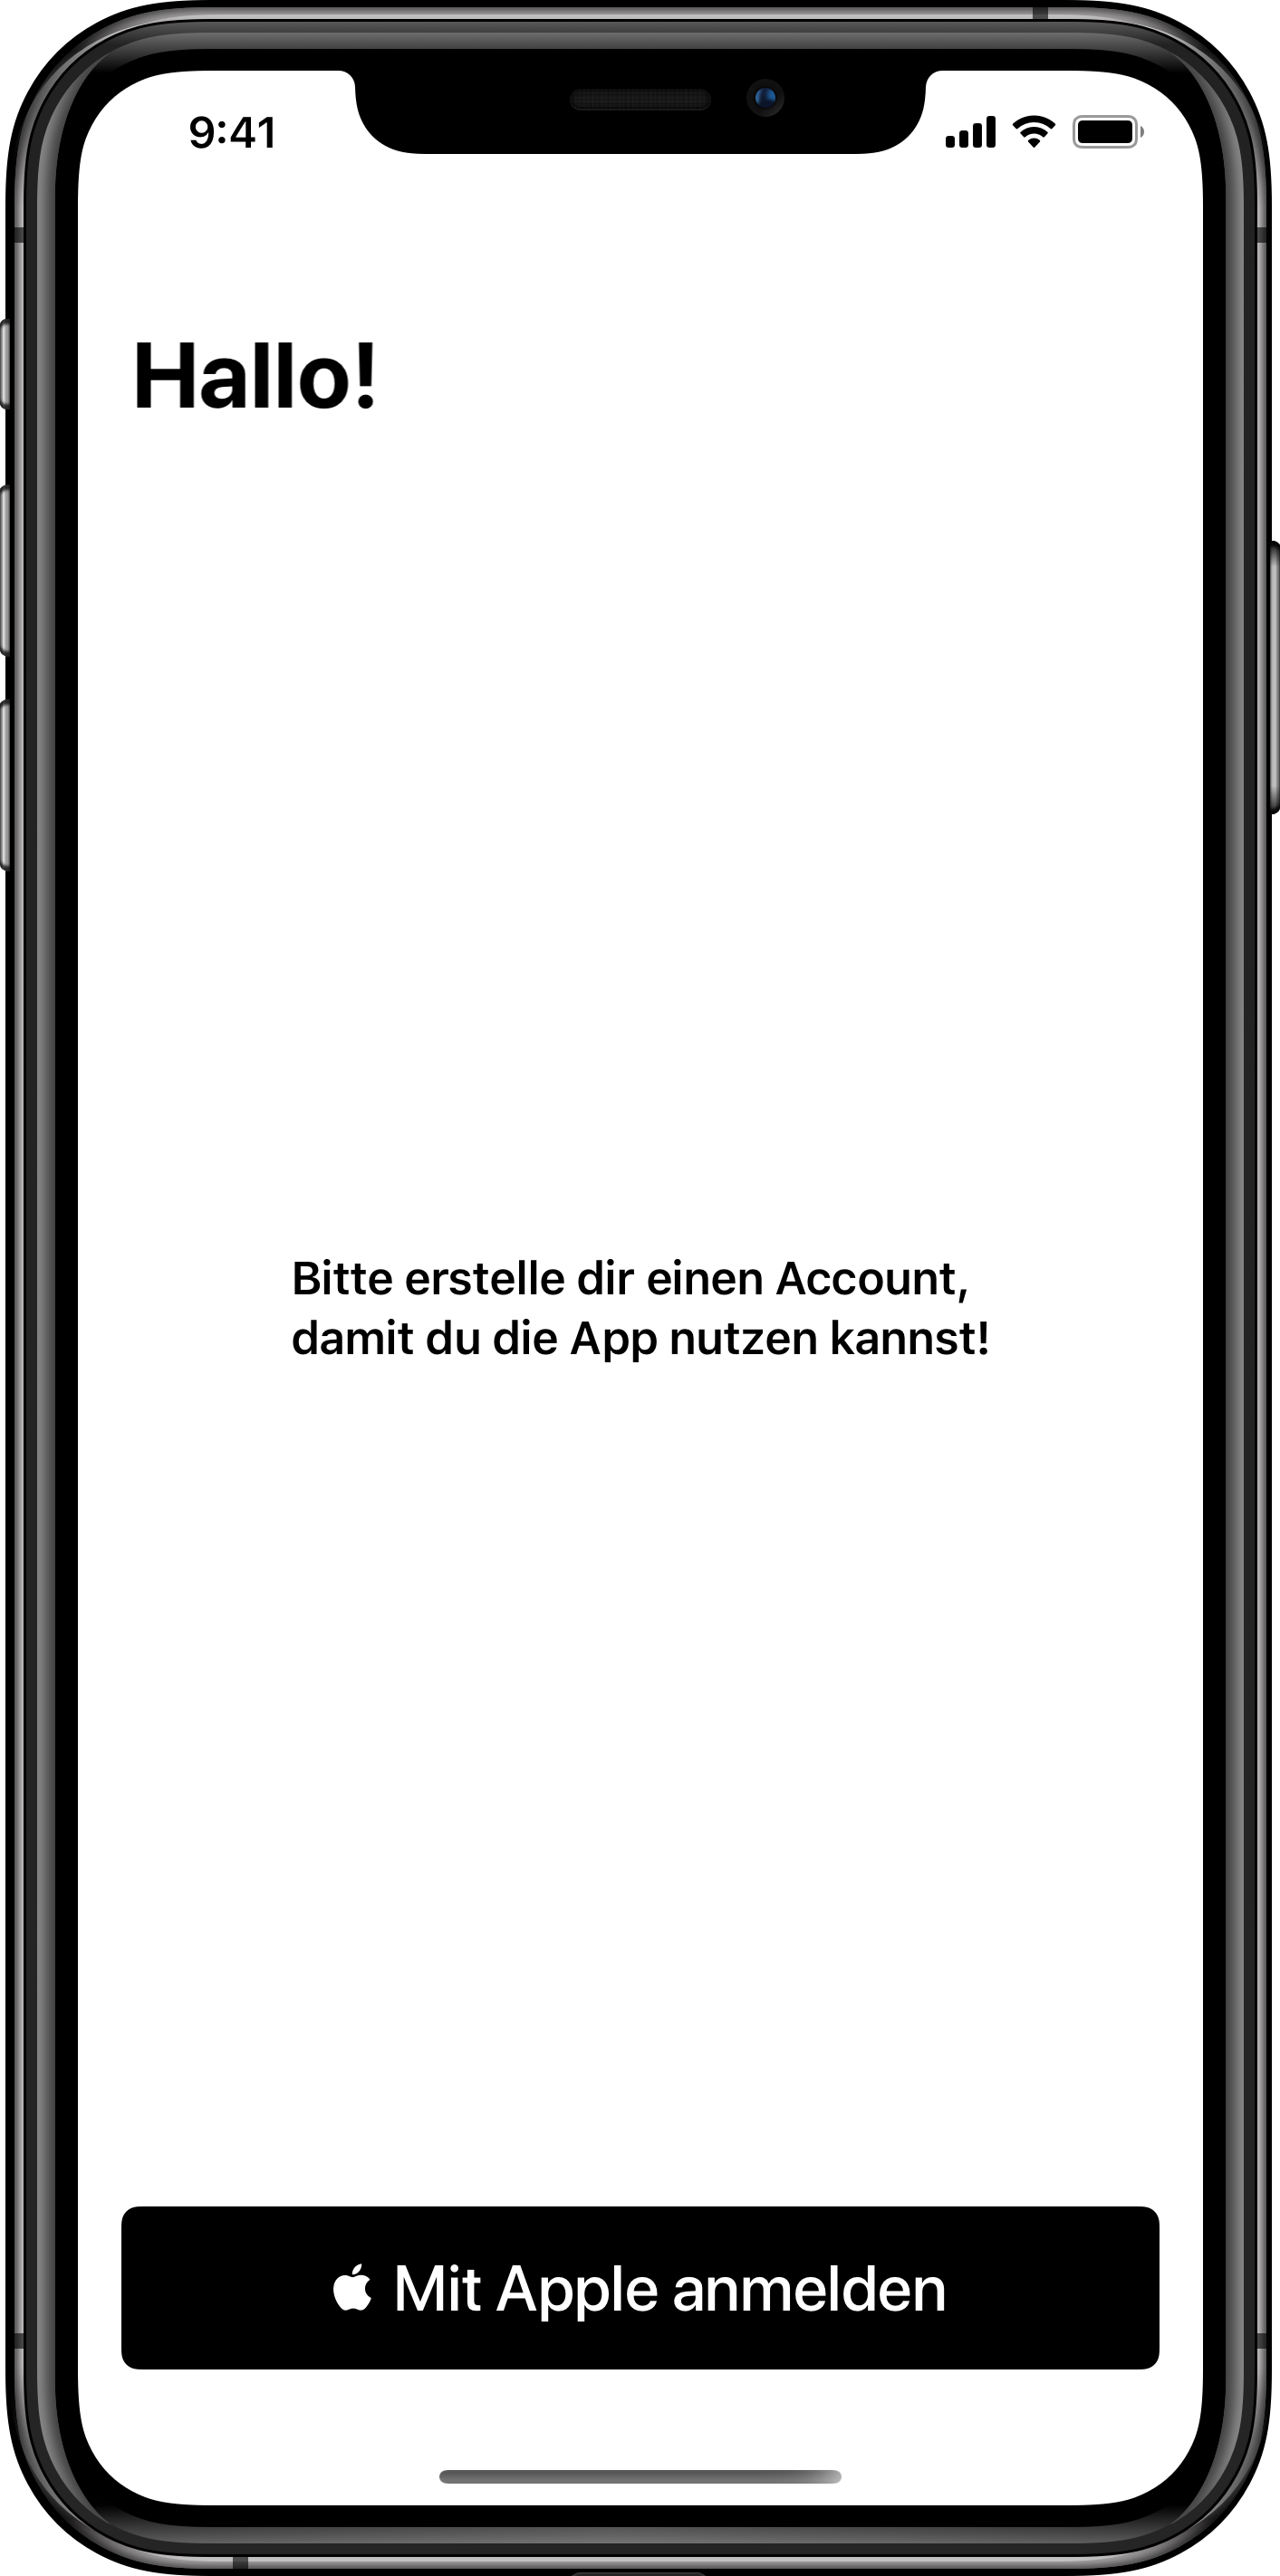
\includegraphics[width=.68\textwidth]{./images/prototype/ios/loginNoAccount.png}
		\caption{\label{fig:app:ios:loginNoAccount}Login-Screen. Benutzer hat noch keinen Account angelegt.}
	\end{figure}
\end{minipage}\hfill
\begin{minipage}{.45\textwidth}
	\begin{figure}[H]
		\centering
		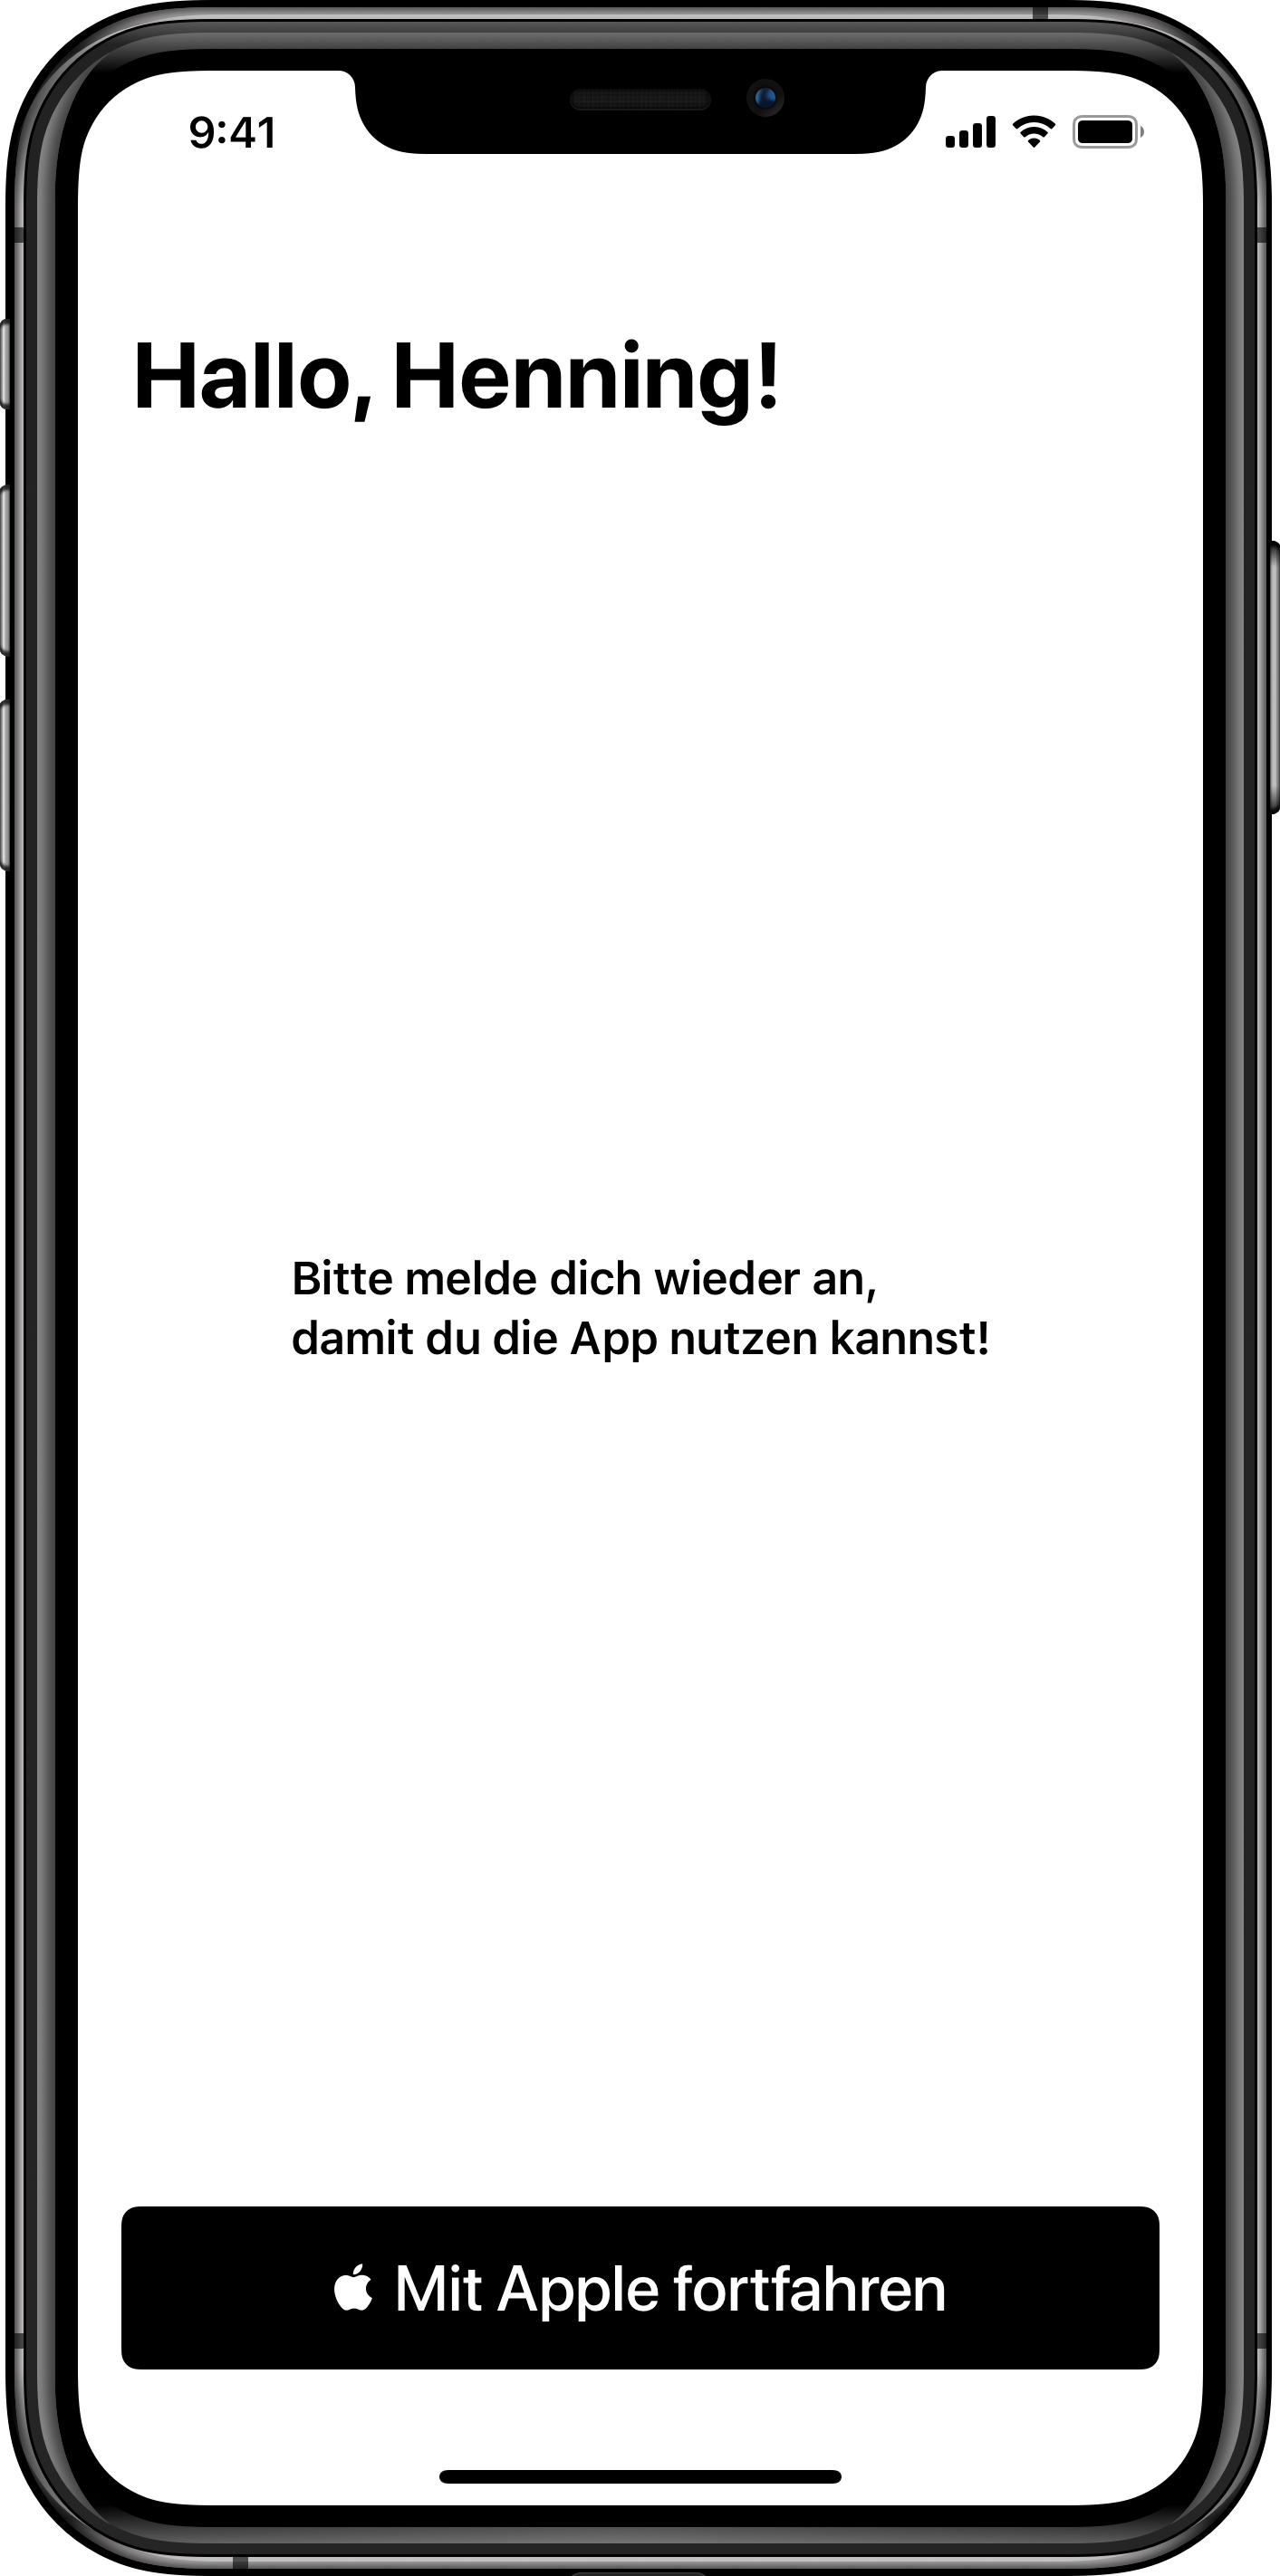
\includegraphics[width=.68\textwidth]{./images/prototype/ios/loginWithAccount.png}
		\caption{\label{fig:app:ios:loginWithAccount}Login-Screen. Benutzer hat bereits einen Account angelegt.}
	\end{figure}
\end{minipage}\clearpage

\begin{minipage}{.45\textwidth}
	\begin{figure}[H]
		\centering
		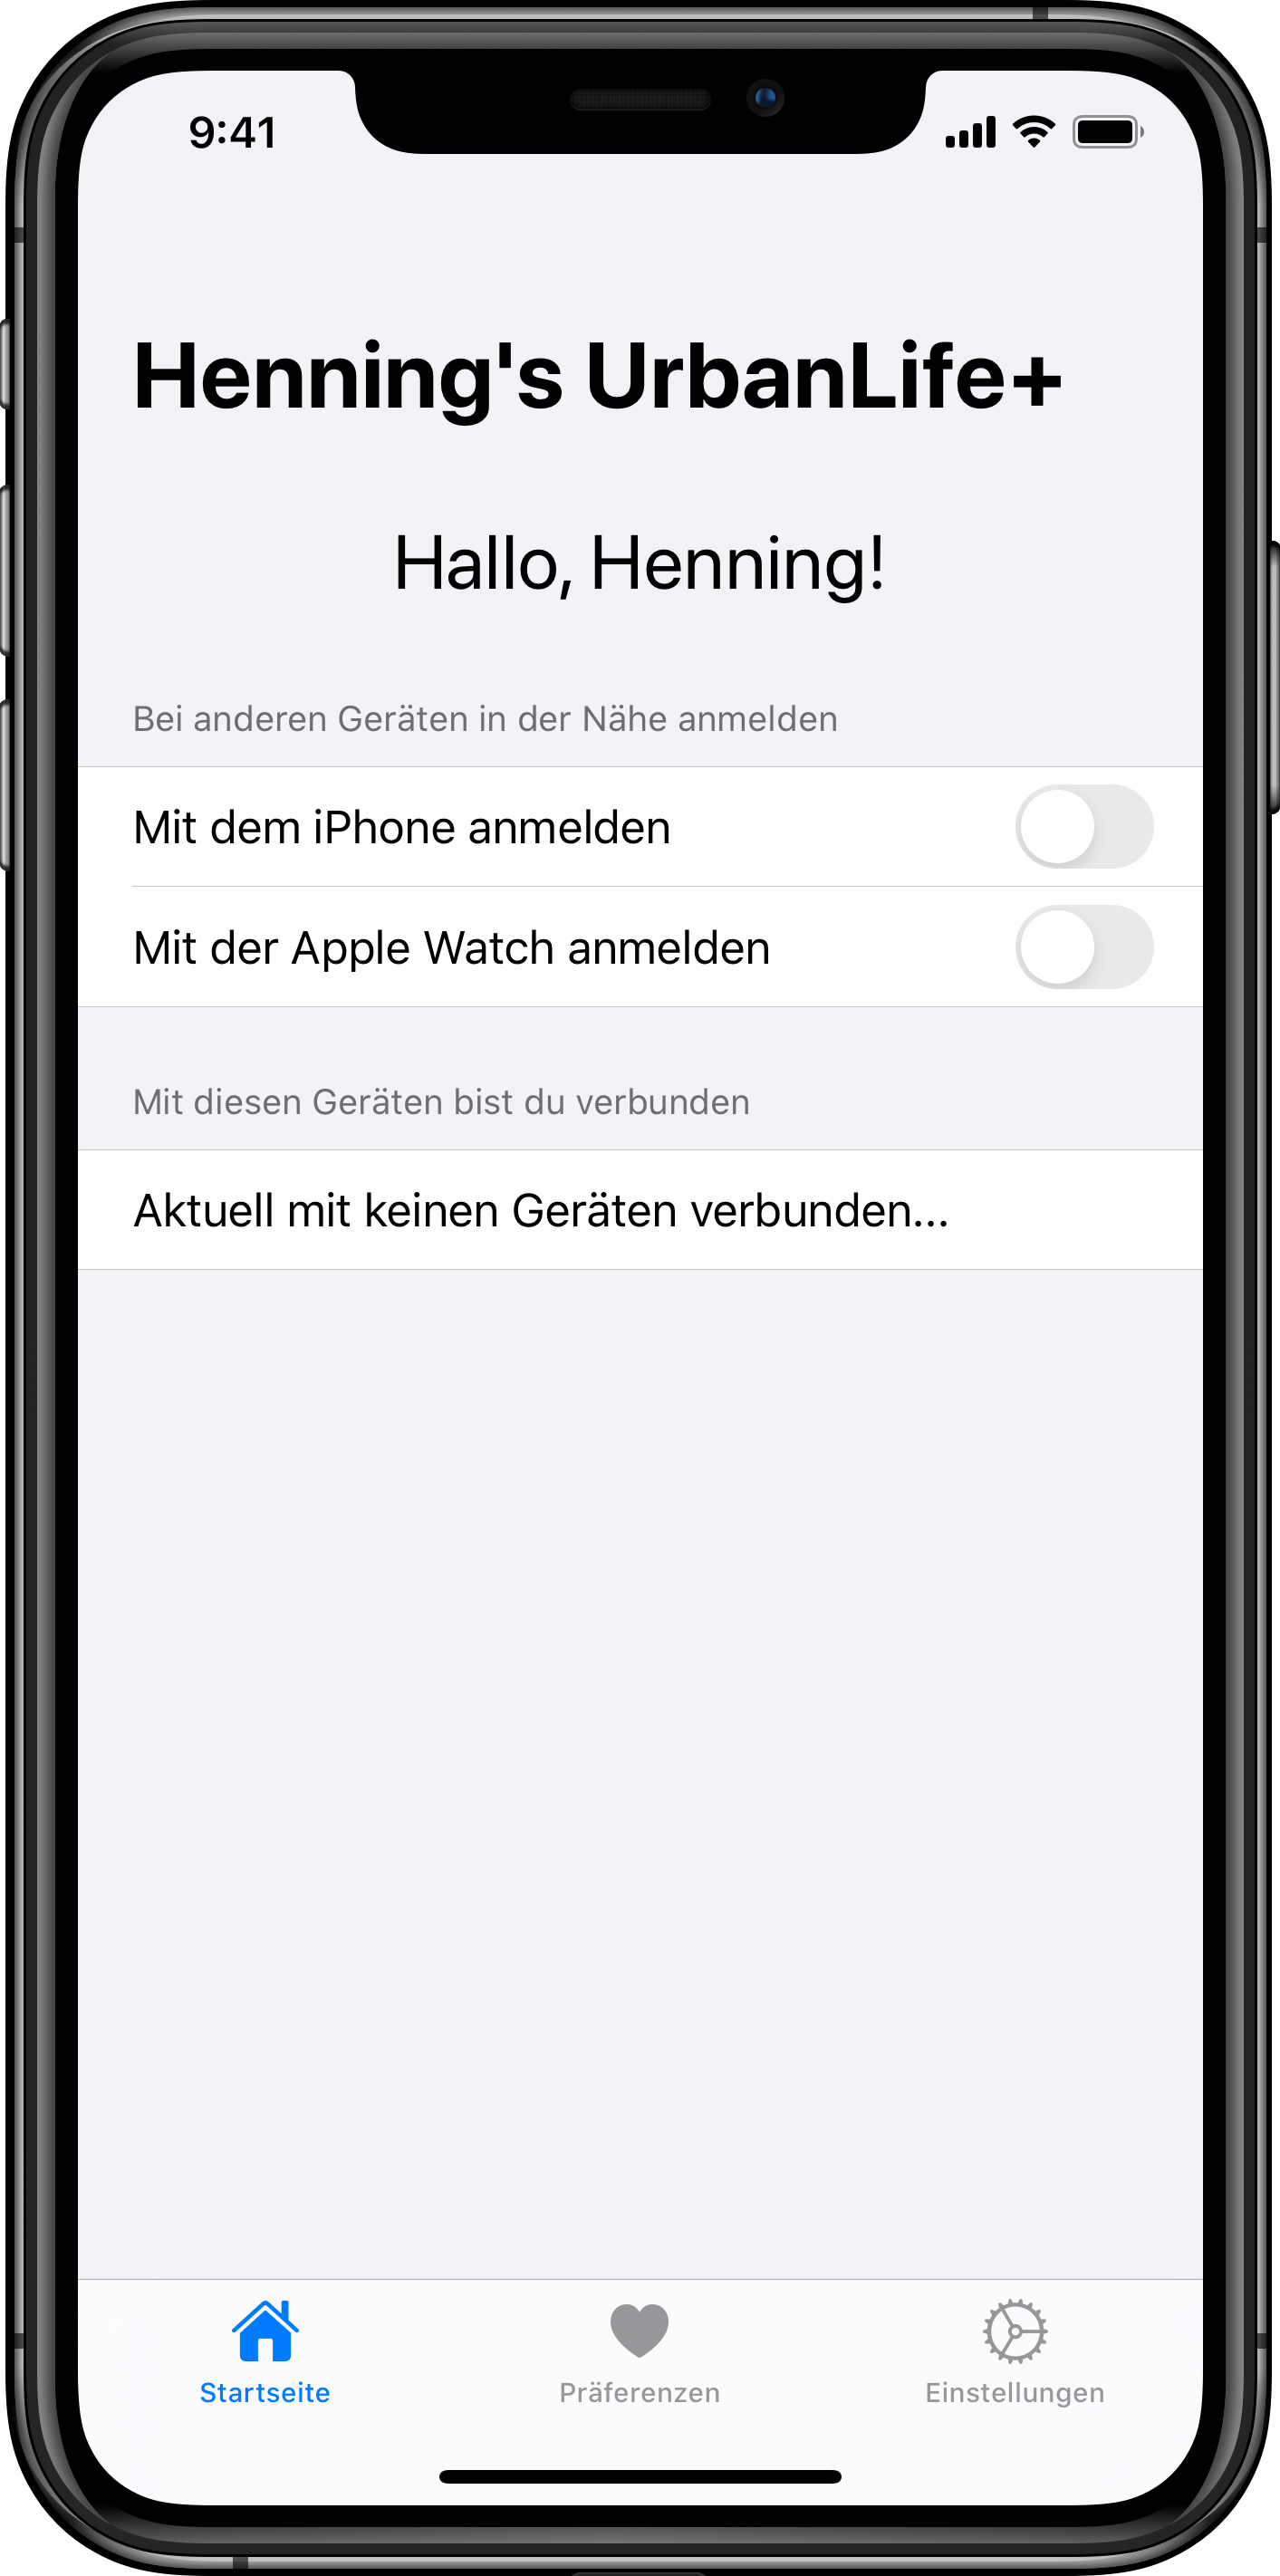
\includegraphics[width=.68\textwidth]{./images/prototype/ios/home.png}
		\caption{\label{fig:app:ios:home}Startseite. Kein Gerät verbunden.}
	\end{figure}
\end{minipage}\hfill
\begin{minipage}{.45\textwidth}
	\begin{figure}[H]
		\centering
		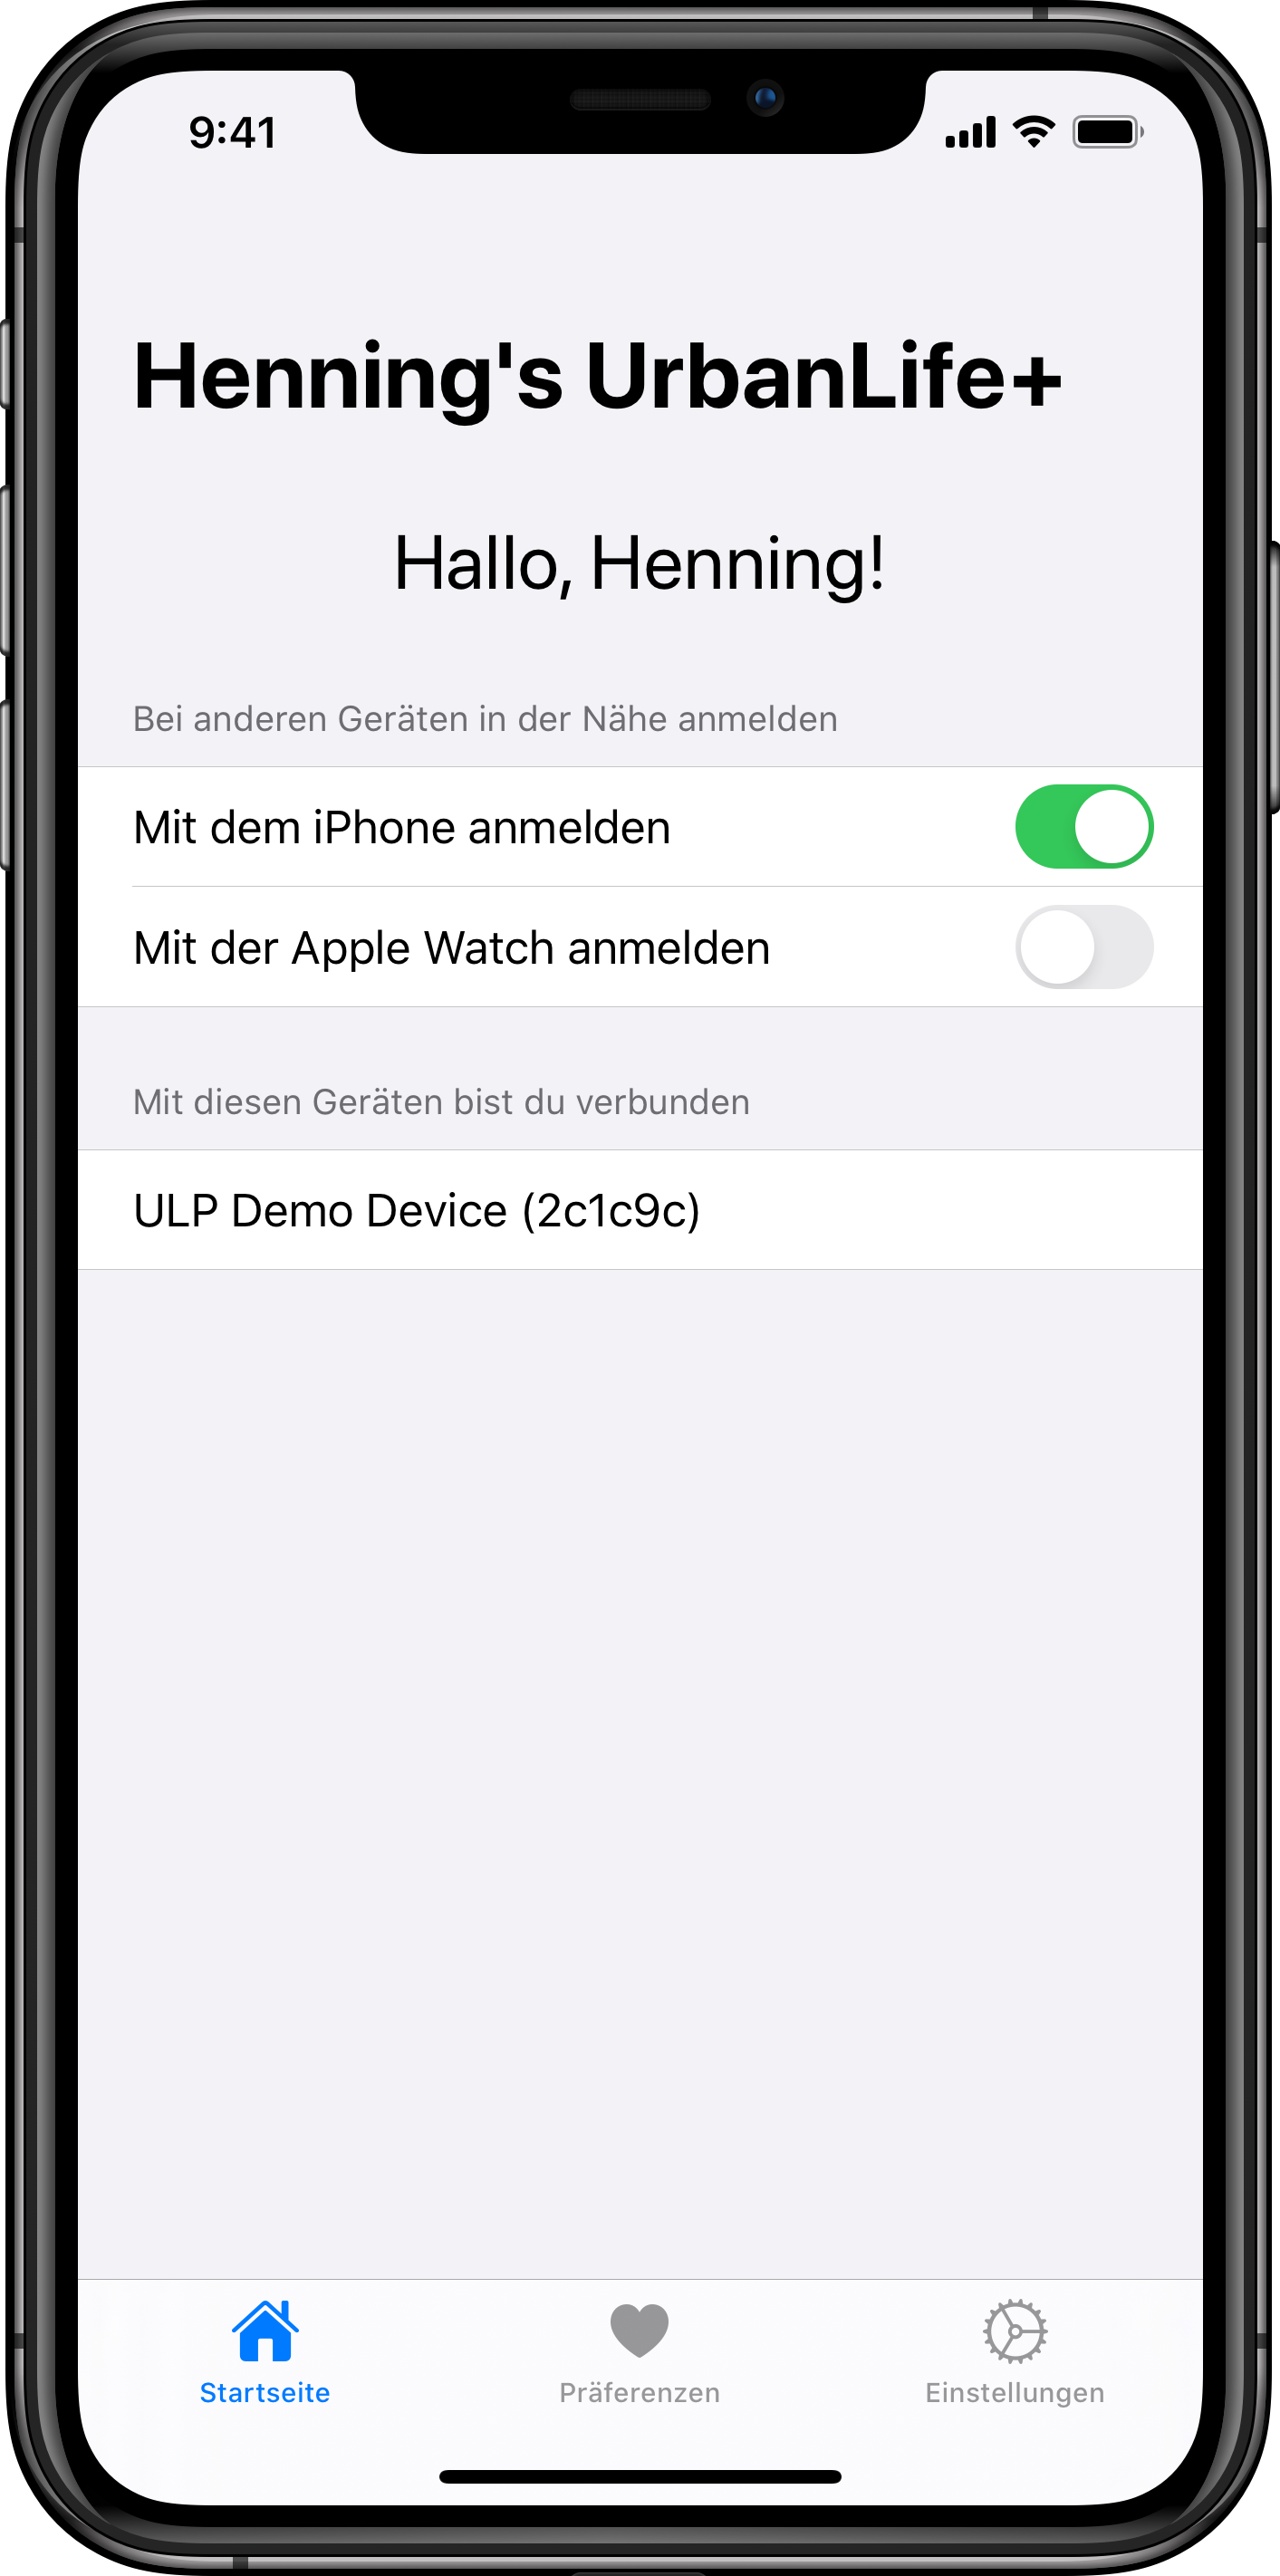
\includegraphics[width=.68\textwidth]{./images/prototype/ios/homeConnected.png}
		\caption{\label{fig:app:ios:homeConnected}Startseite mit verbundenem Gerät.}
	\end{figure}
\end{minipage}

\begin{minipage}{.45\textwidth}
	\begin{figure}[H]
		\centering
		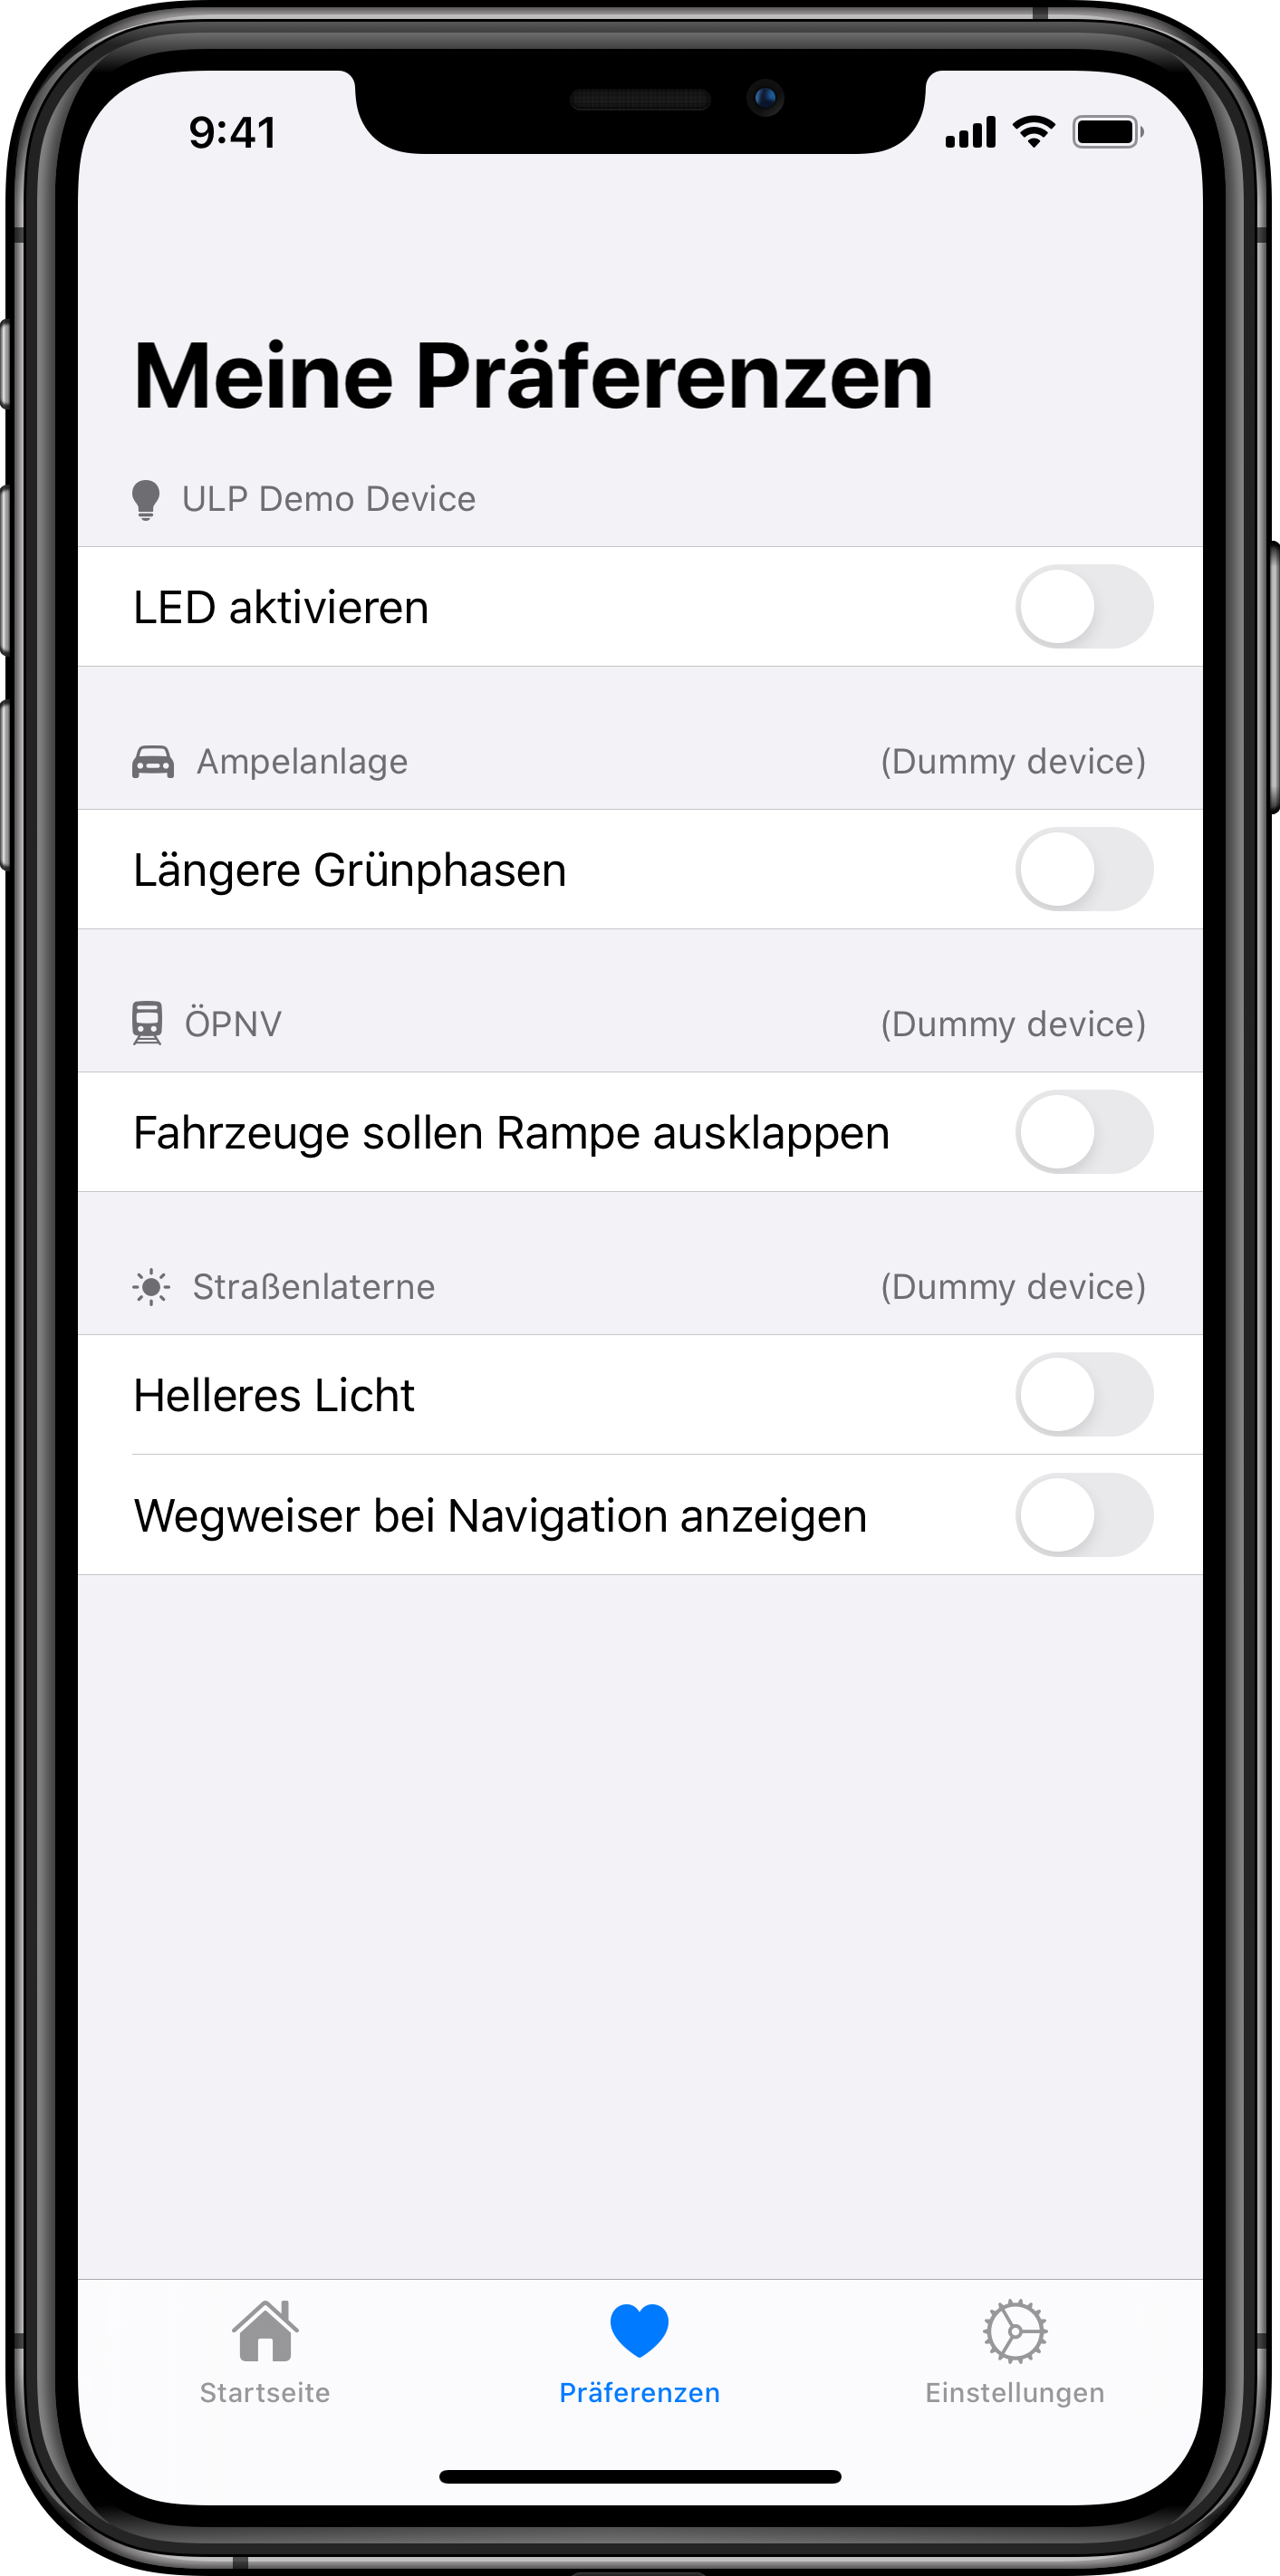
\includegraphics[width=.68\textwidth]{./images/prototype/ios/prefs.png}
		\caption{\label{fig:app:ios:prefs}Präferenzen festlegen.}
	\end{figure}
\end{minipage}\hfill
\begin{minipage}{.45\textwidth}
	\begin{figure}[H]
		\centering
		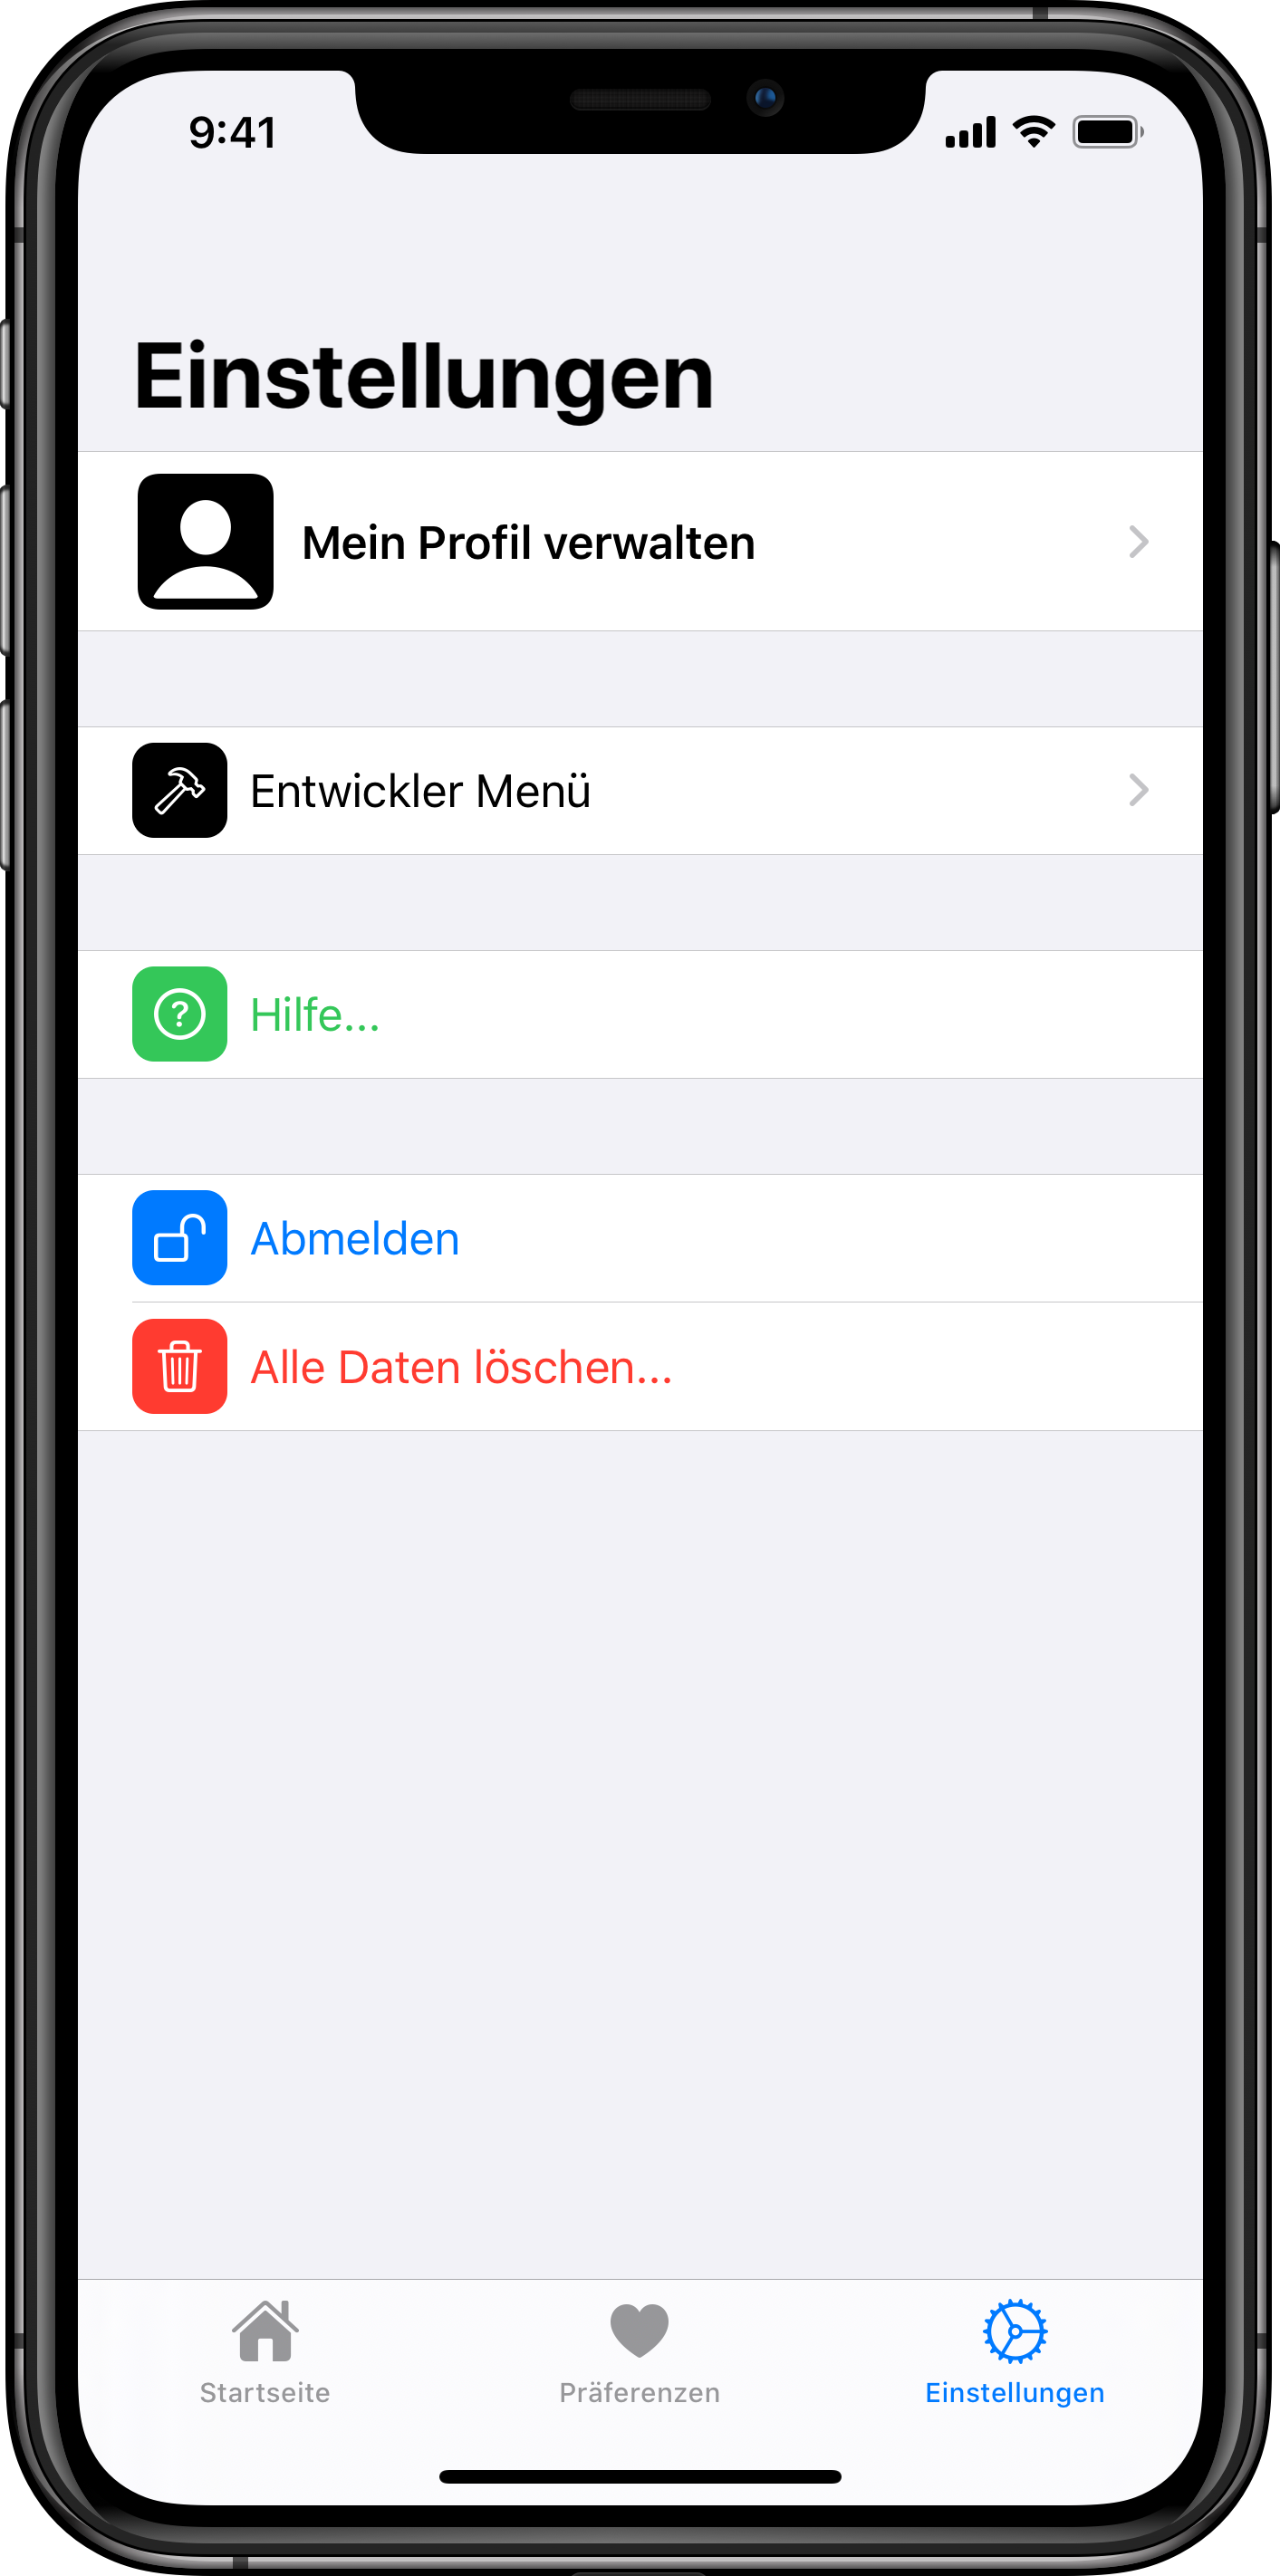
\includegraphics[width=.68\textwidth]{./images/prototype/ios/settings.png}
		\caption{\label{fig:app:ios:settings}Einstellungen der App.}
	\end{figure}
\end{minipage}

\begin{minipage}{.45\textwidth}
	\begin{figure}[H]
		\centering
		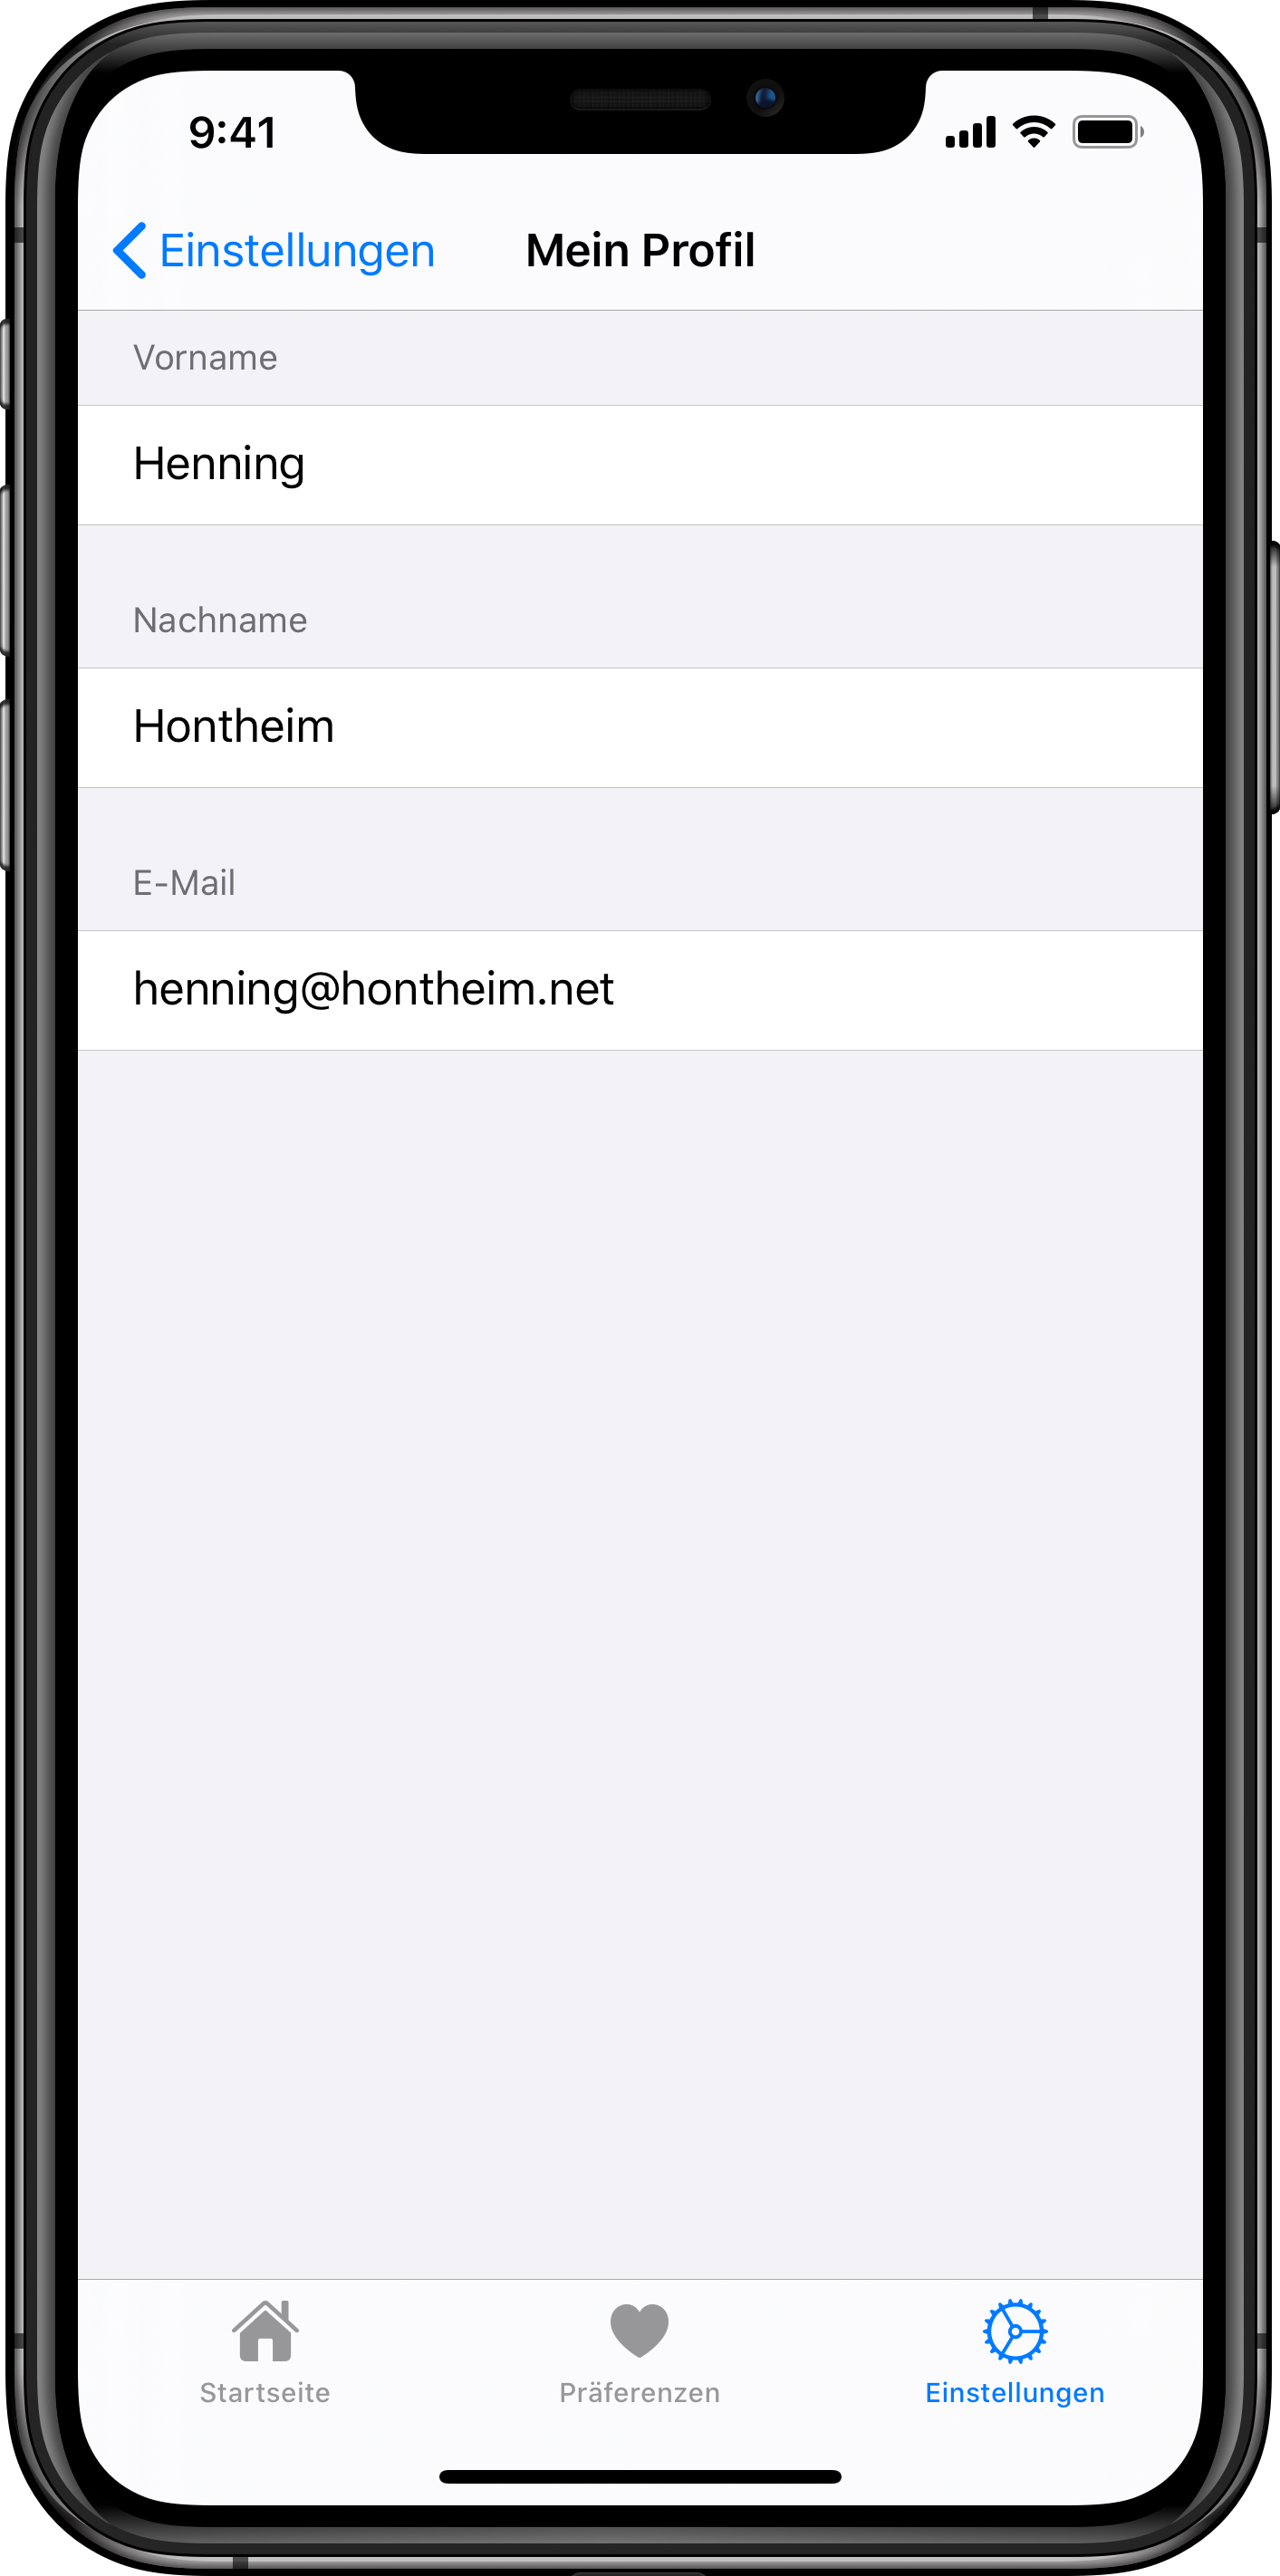
\includegraphics[width=.68\textwidth]{./images/prototype/ios/profile.png}
		\caption{\label{fig:app:ios:profile}Mein Profil verwalten.}
	\end{figure}
\end{minipage}\hfill
\begin{minipage}{.45\textwidth}
	\begin{figure}[H]
		\centering
		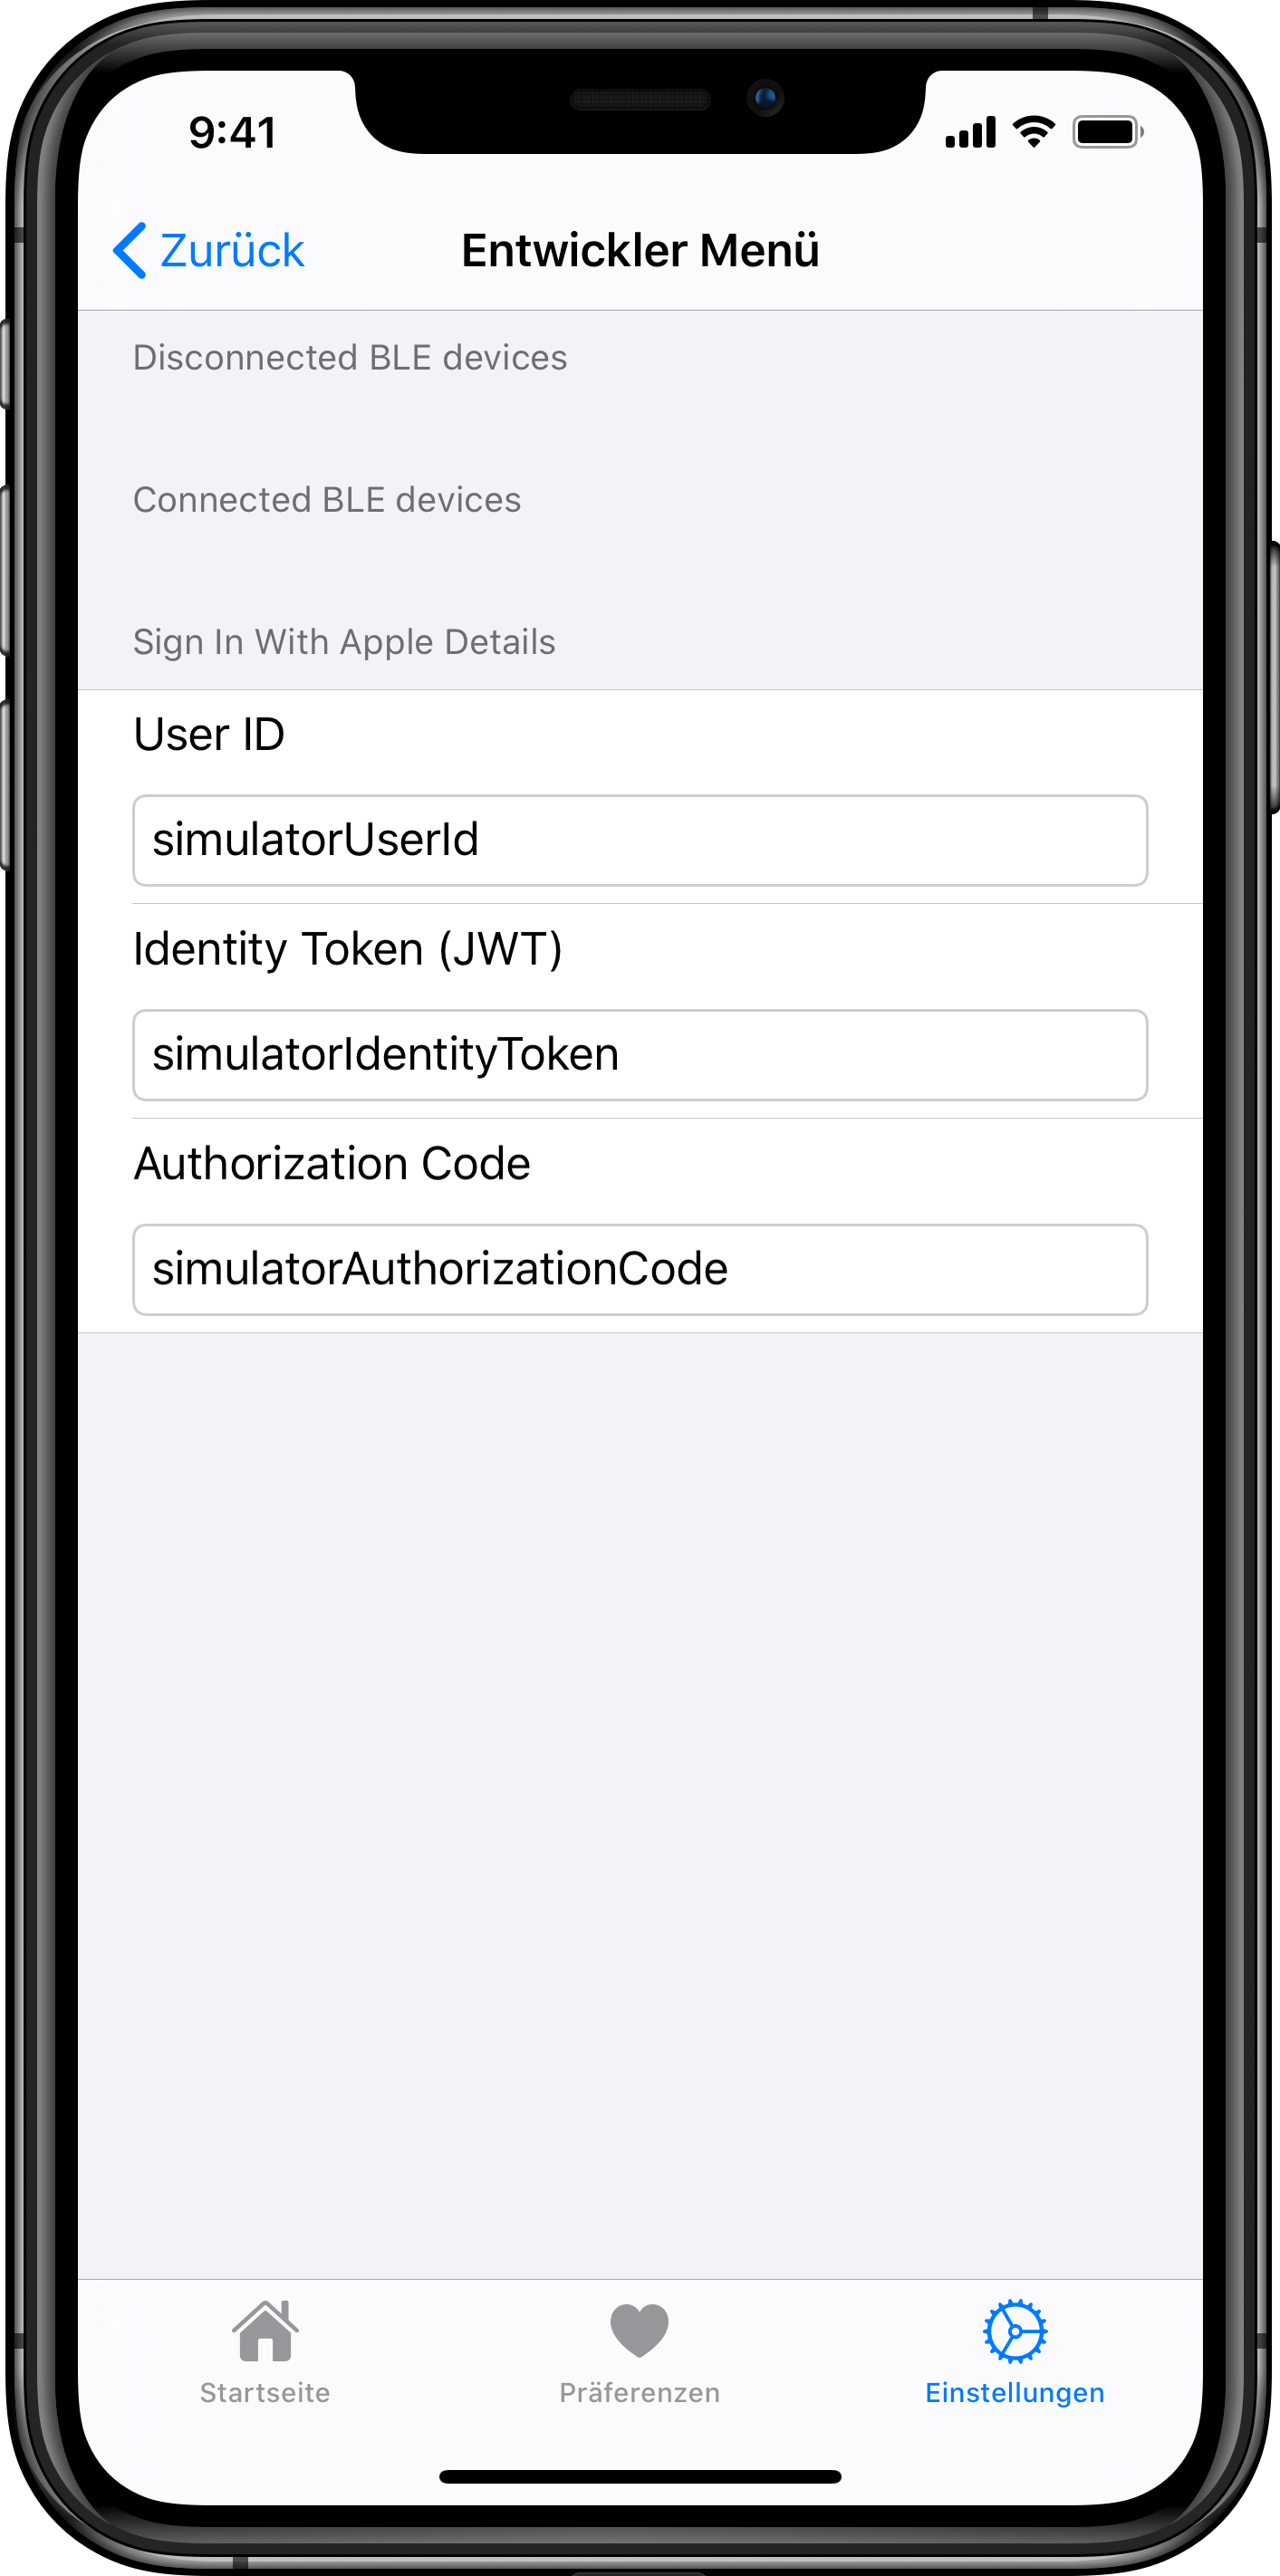
\includegraphics[width=.68\textwidth]{./images/prototype/ios/dev.png}
		\caption{\label{fig:app:ios:dev}Das Entwickler Menü.}
	\end{figure}
\end{minipage}

\begin{minipage}{.45\textwidth}
	\begin{figure}[H]
		\centering
		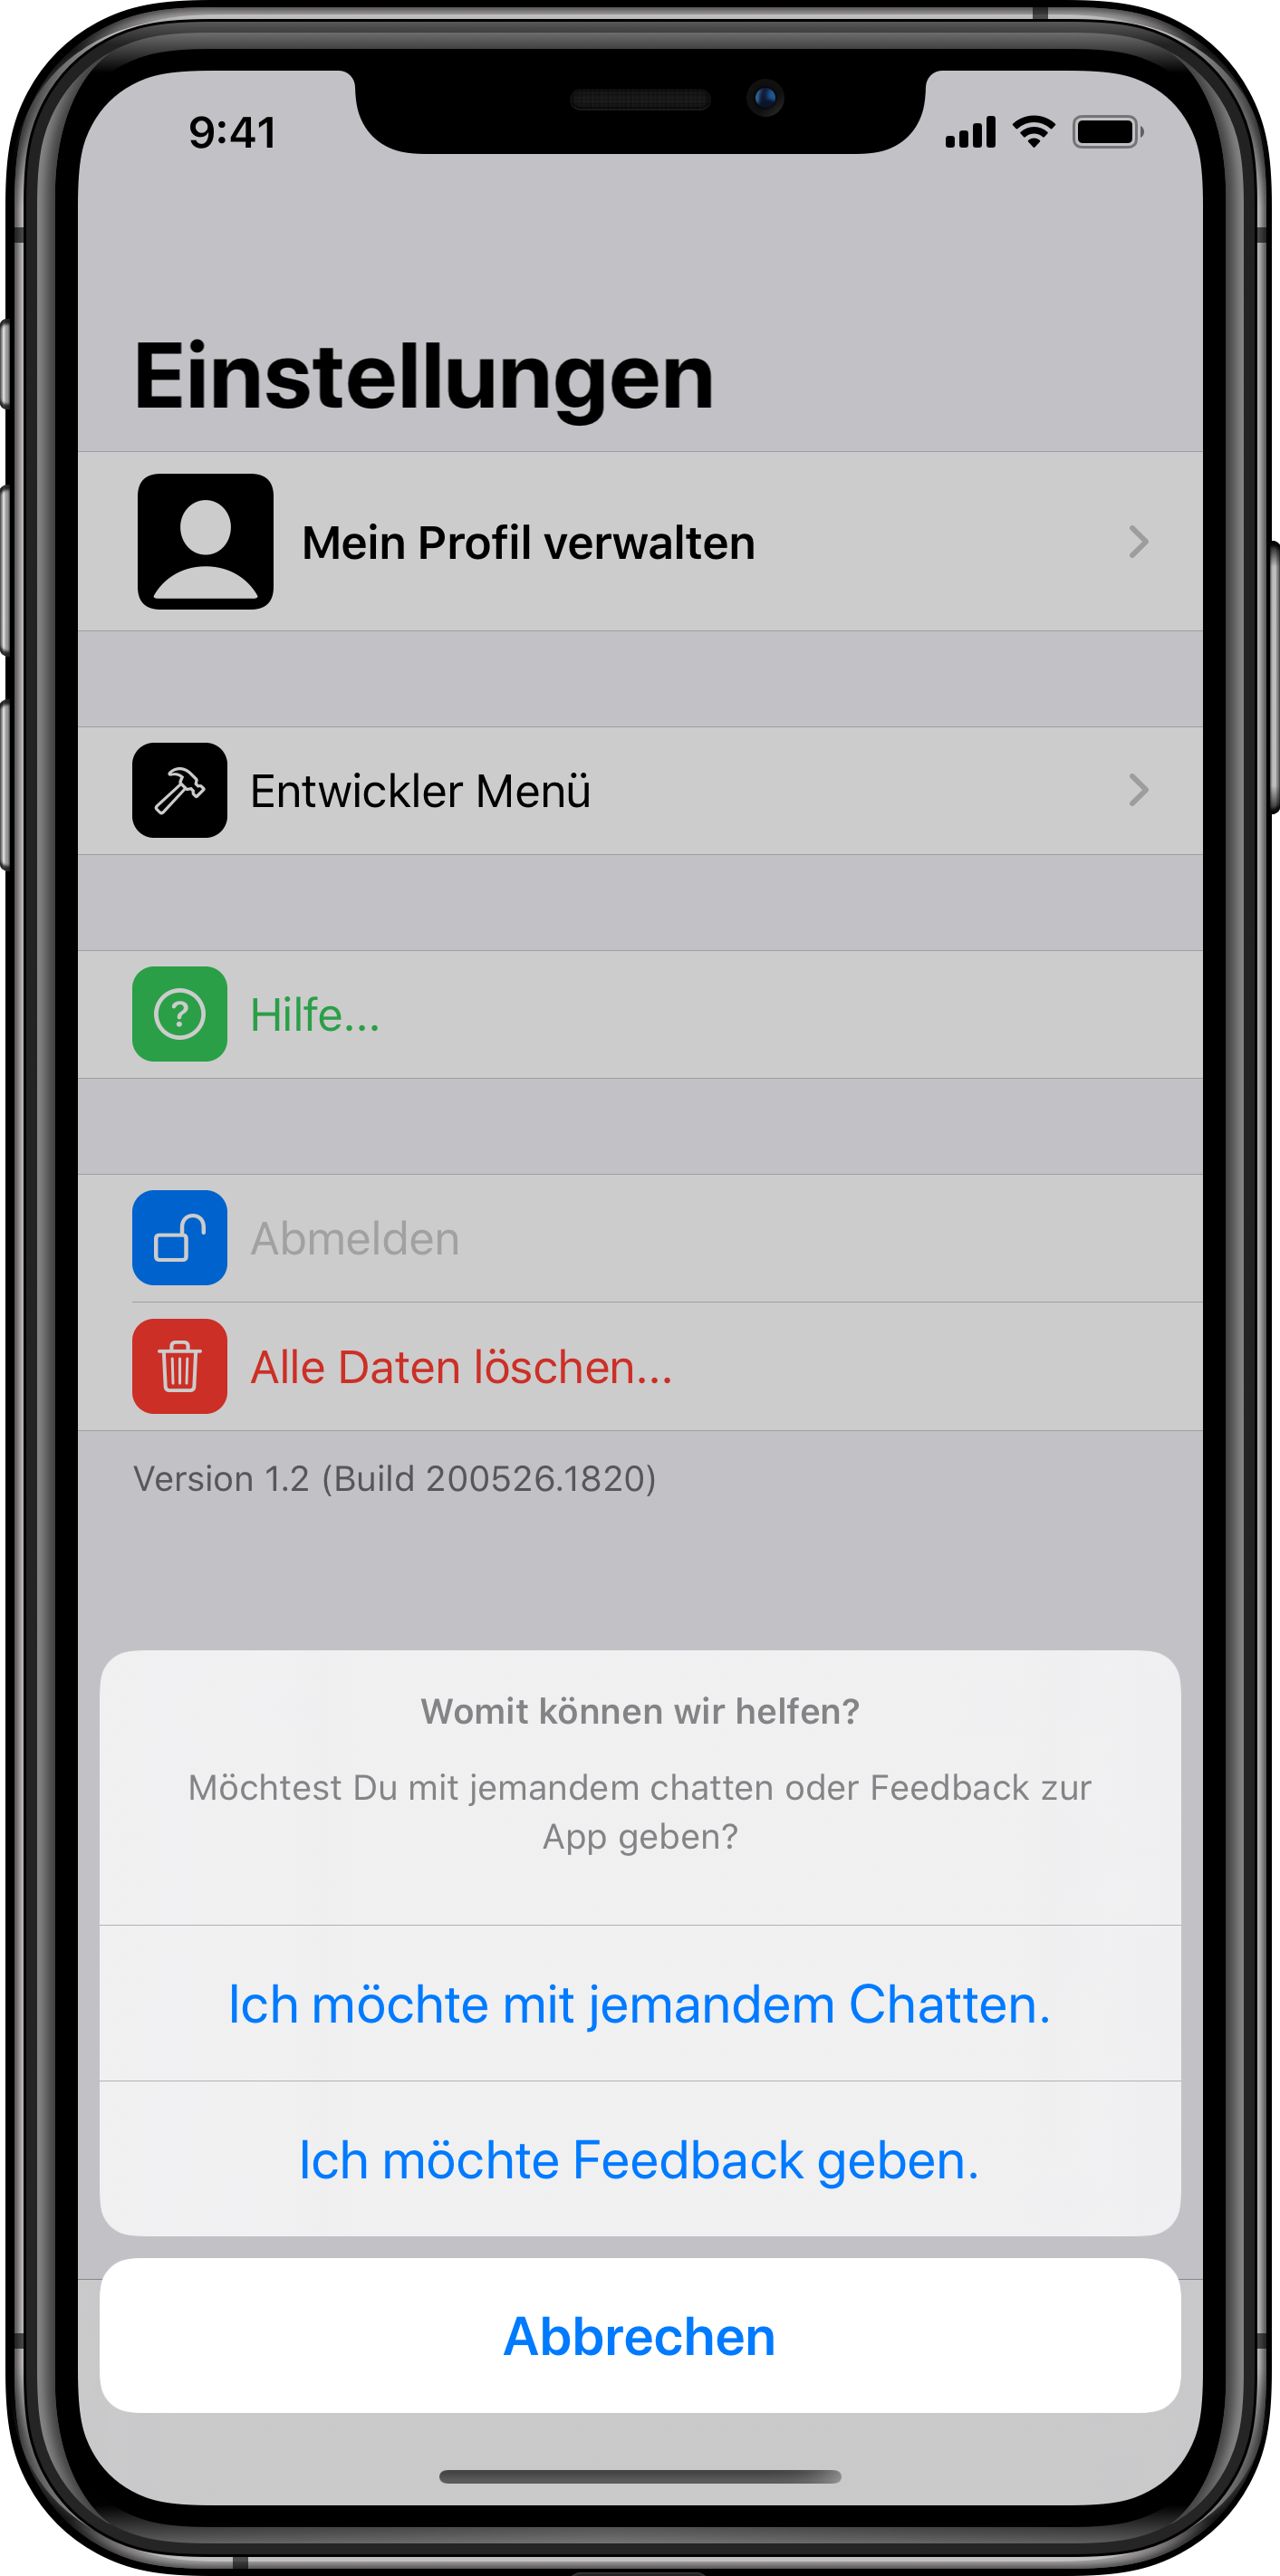
\includegraphics[width=.68\textwidth]{./images/prototype/ios/helpSheet.png}
		\caption{\label{fig:app:ios:helpSheet}Der Hilfe-Hinweis.}
	\end{figure}
\end{minipage}\hfill
\begin{minipage}{.45\textwidth}
	\begin{figure}[H]
		\centering
		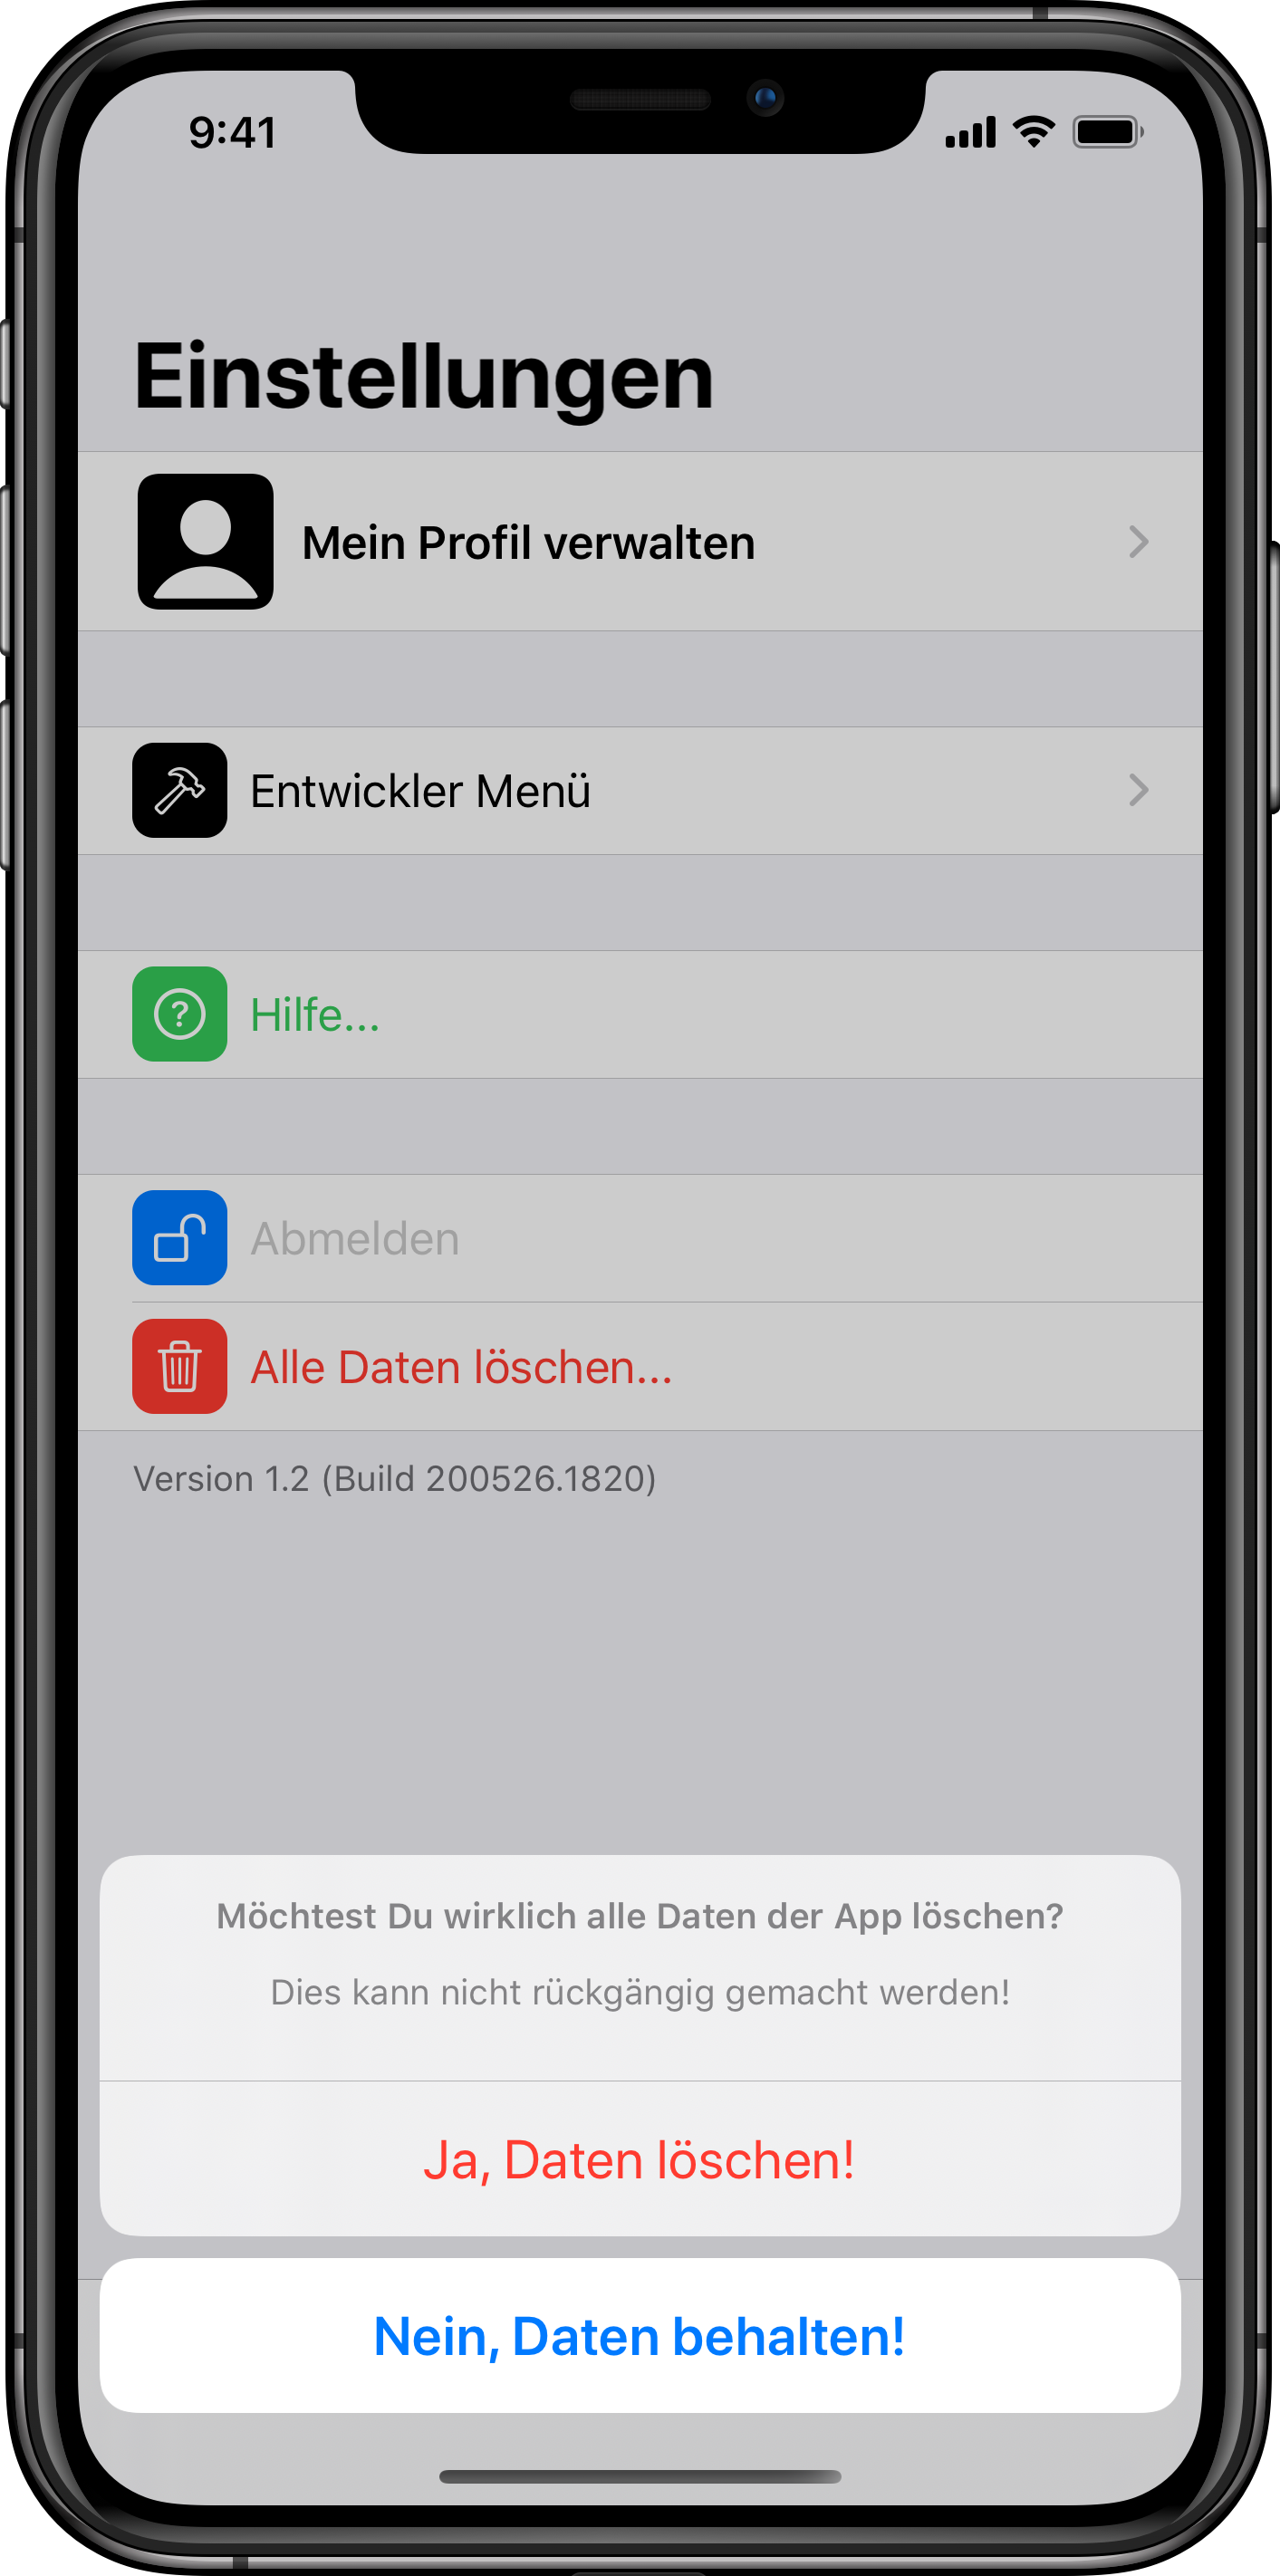
\includegraphics[width=.68\textwidth]{./images/prototype/ios/nukeSheet.png}
		\caption{\label{fig:app:ios:nukeSheet}Bestätigung der Datenlöschung.}
	\end{figure}
\end{minipage}

\begin{minipage}{.45\textwidth}
	\begin{figure}[H]
		\centering
		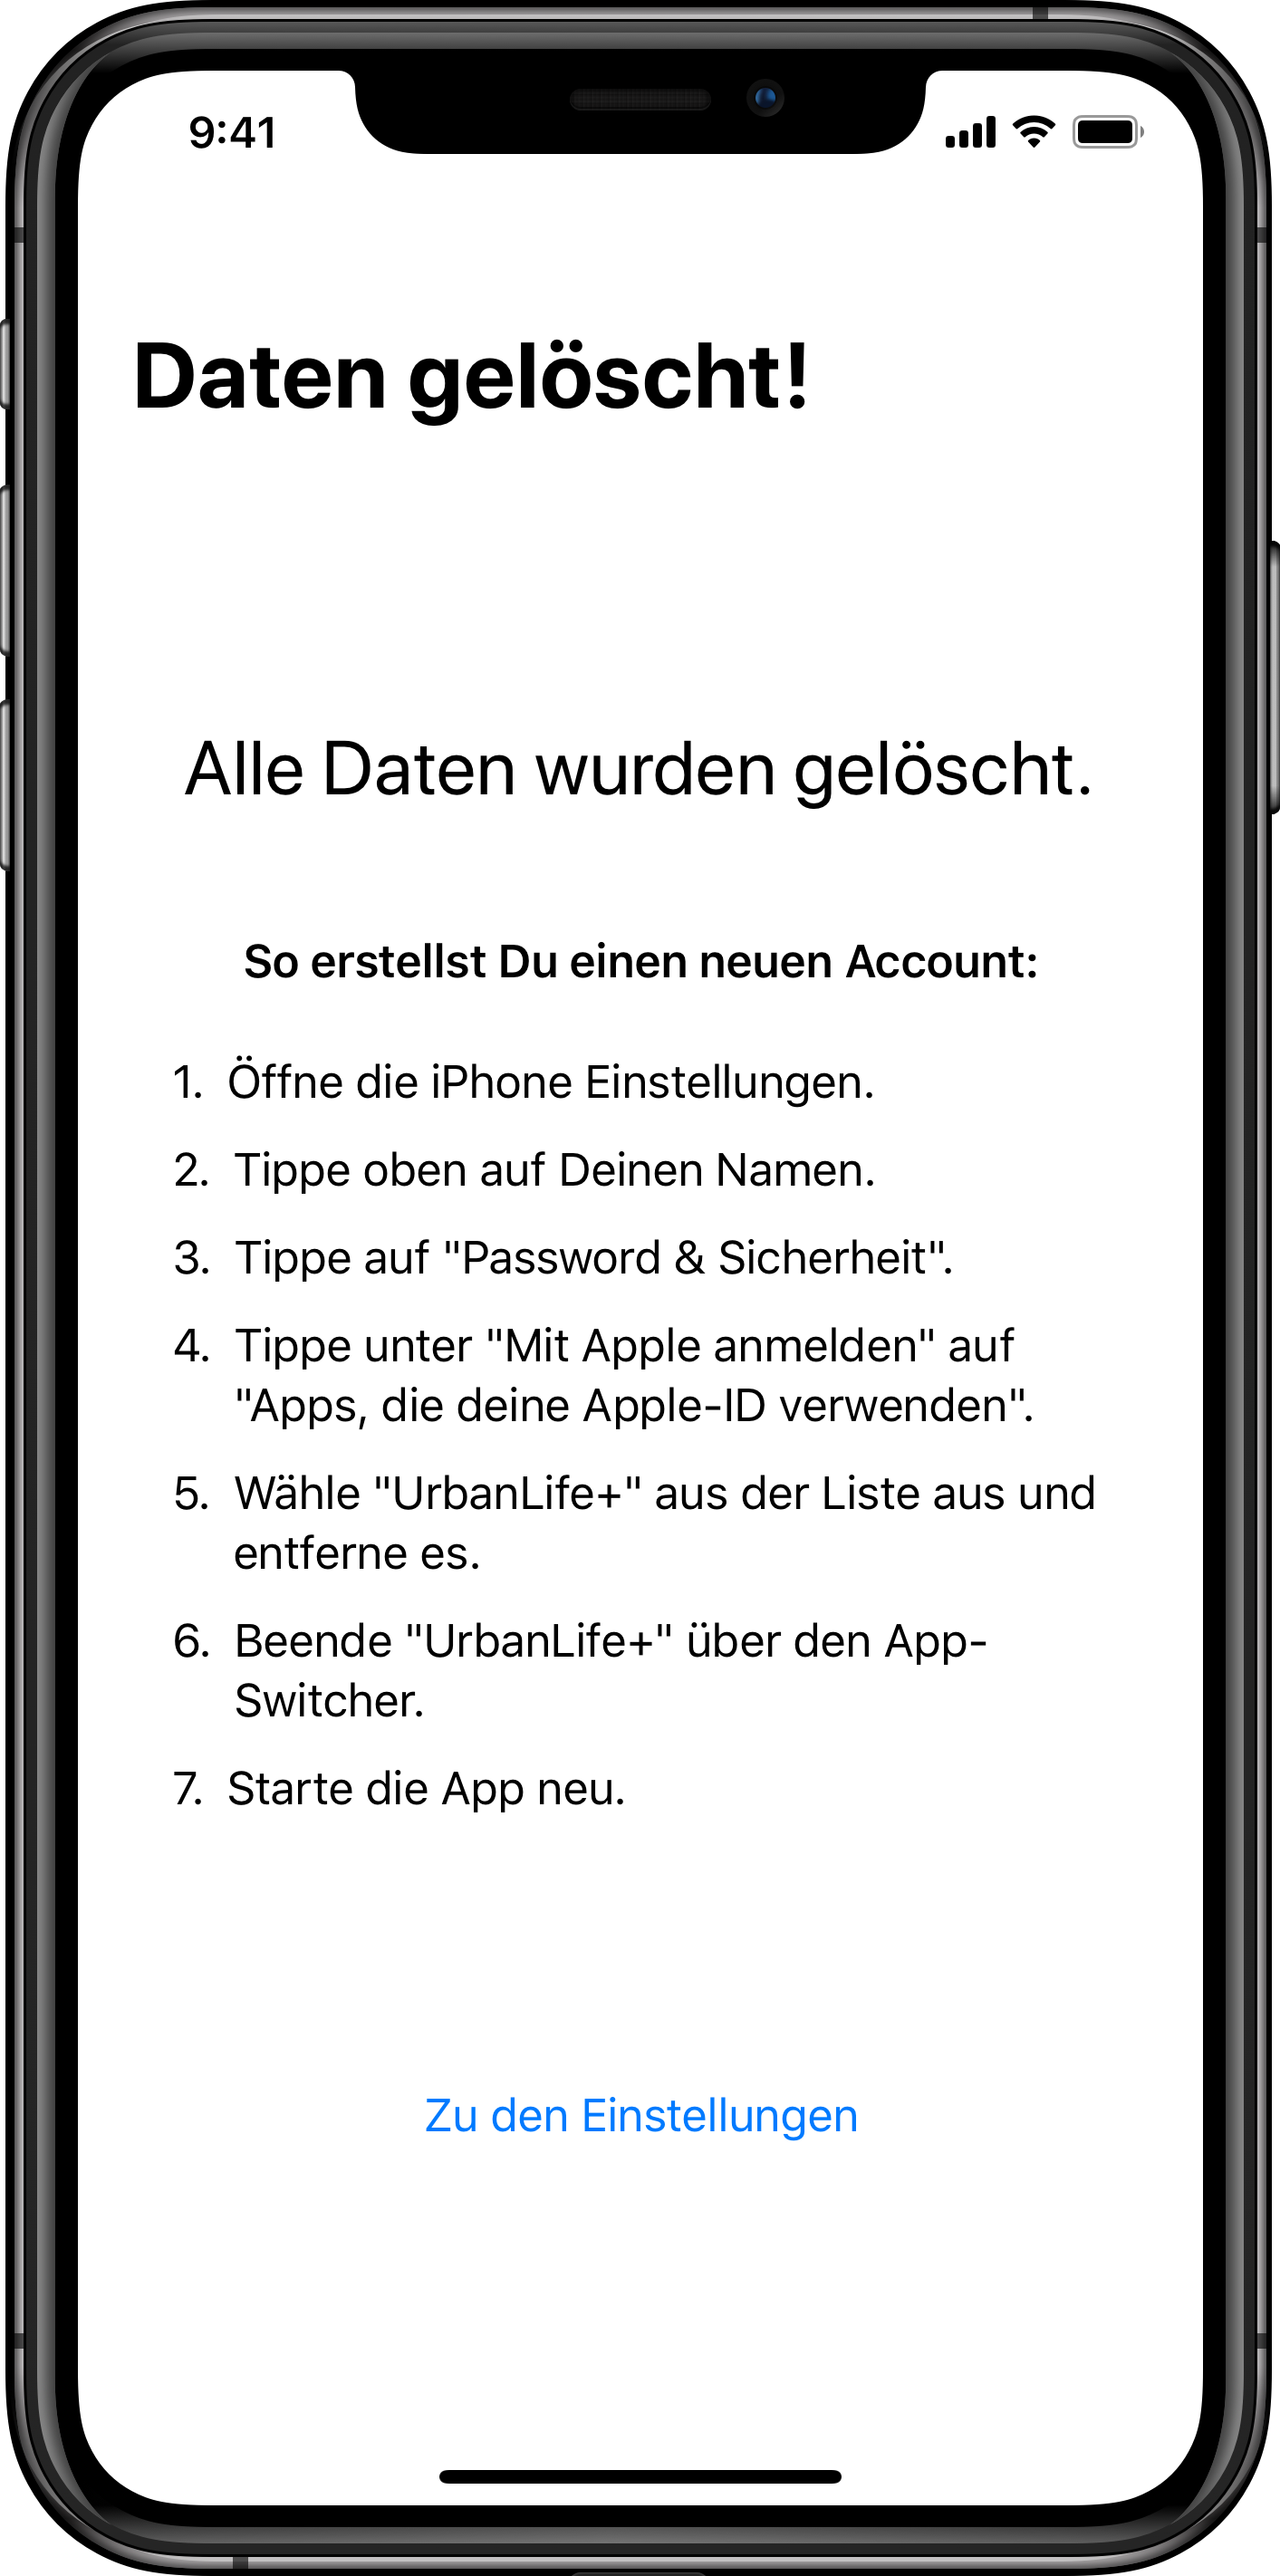
\includegraphics[width=.68\textwidth]{./images/prototype/ios/nuked.png}
		\caption{\label{fig:app:ios:nuked}Abschluss des Löschvorgangs.}
	\end{figure}
\end{minipage}

\subsection{watchOS App}

\begin{minipage}{.45\textwidth}
	\begin{figure}[H]
		\centering
		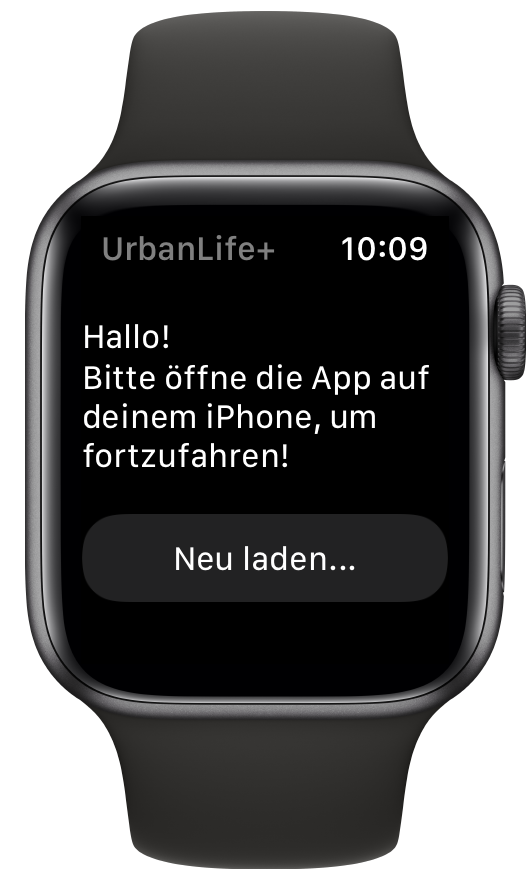
\includegraphics[width=.68\textwidth]{./images/prototype/watchos/loginNoAccount.png}
		\caption{\label{fig:app:watchos:loginNoAccount}Login-Screen. Benutzer hat noch keinen Account angelegt.}
	\end{figure}
\end{minipage}\hfill
\begin{minipage}{.45\textwidth}
	\begin{figure}[H]
		\centering
		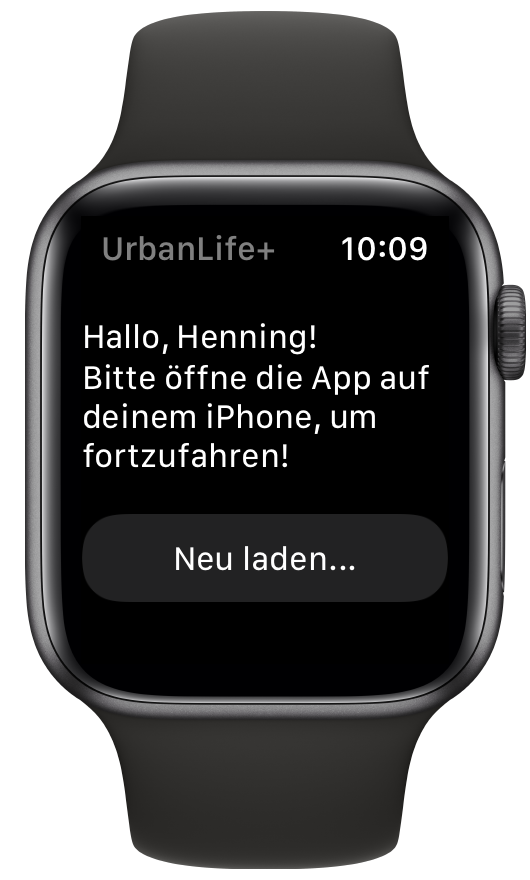
\includegraphics[width=.68\textwidth]{./images/prototype/watchos/loginWithAccount.png}
		\caption{\label{fig:app:watchos:loginWithAccount}Login-Screen. Benutzer hat bereits einen Account angelegt.}
	\end{figure}
\end{minipage}

\begin{minipage}{.45\textwidth}
	\begin{figure}[H]
		\centering
		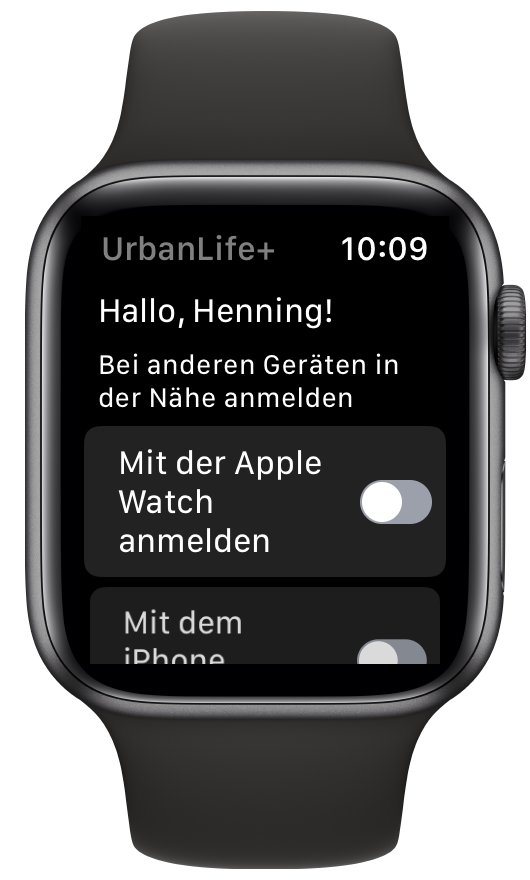
\includegraphics[width=.68\textwidth]{./images/prototype/watchos/home1.png}
		\caption{\label{fig:app:watchos:home1}Startseite. Teil 1.}
	\end{figure}
\end{minipage}\hfill
\begin{minipage}{.45\textwidth}
	\begin{figure}[H]
		\centering
		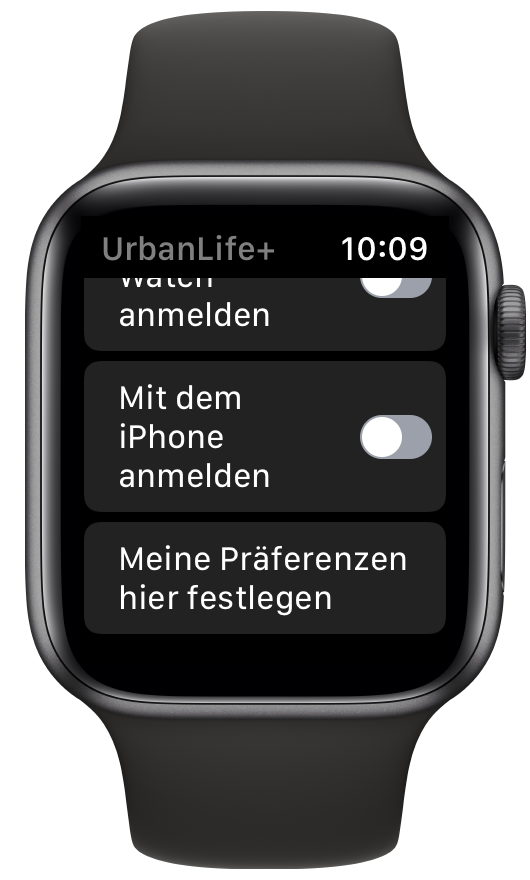
\includegraphics[width=.68\textwidth]{./images/prototype/watchos/home2.png}
		\caption{\label{fig:app:watchos:home2}Startseite. Teil 2.}
	\end{figure}
\end{minipage}

\begin{minipage}{.45\textwidth}
	\begin{figure}[H]
		\centering
		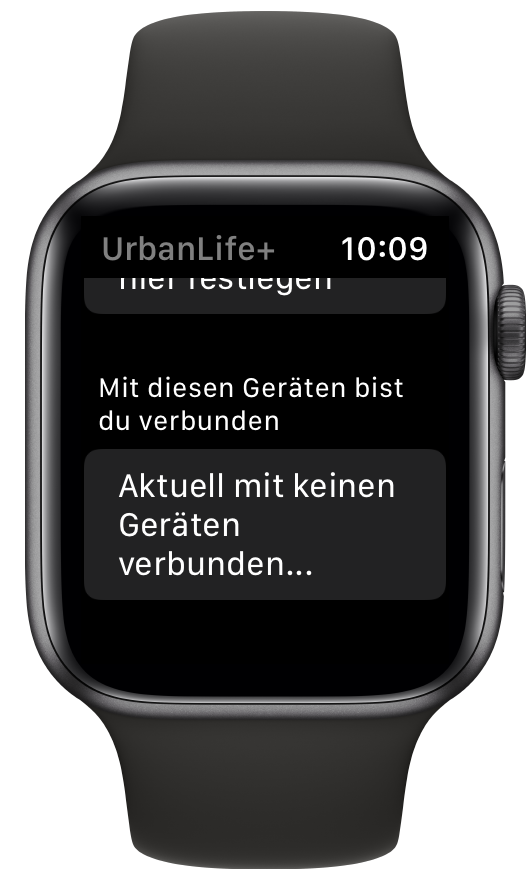
\includegraphics[width=.68\textwidth]{./images/prototype/watchos/homeNotConnected.png}
		\caption{\label{fig:app:watchos:homeNotConnected}Startseite. Uhr ist nicht mit Gerät verbunden.}
	\end{figure}
\end{minipage}\hfill
\begin{minipage}{.45\textwidth}
	\begin{figure}[H]
		\centering
		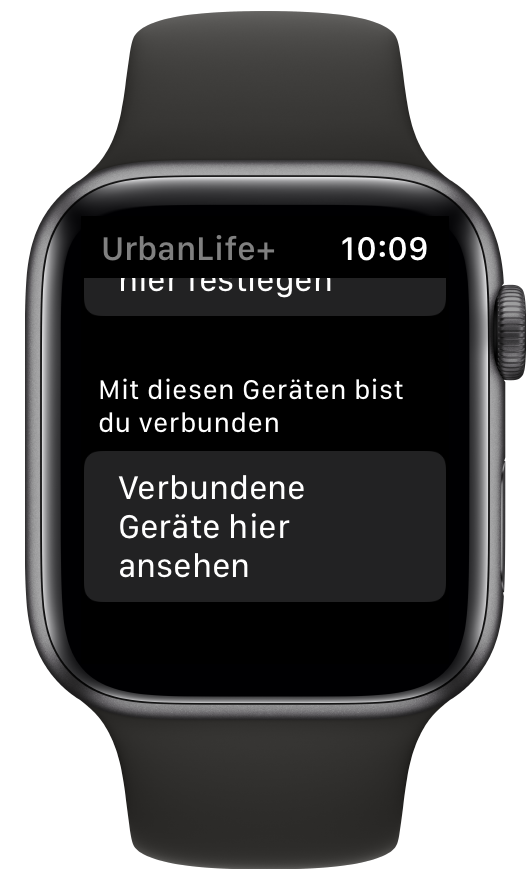
\includegraphics[width=.68\textwidth]{./images/prototype/watchos/homeIsConnected.png}
		\caption{\label{fig:app:watchos:homeIsConnected}Startseite. Uhr ist mit einem Gerät verbunden.}
	\end{figure}
\end{minipage}

\begin{minipage}{.45\textwidth}
	\begin{figure}[H]
		\centering
		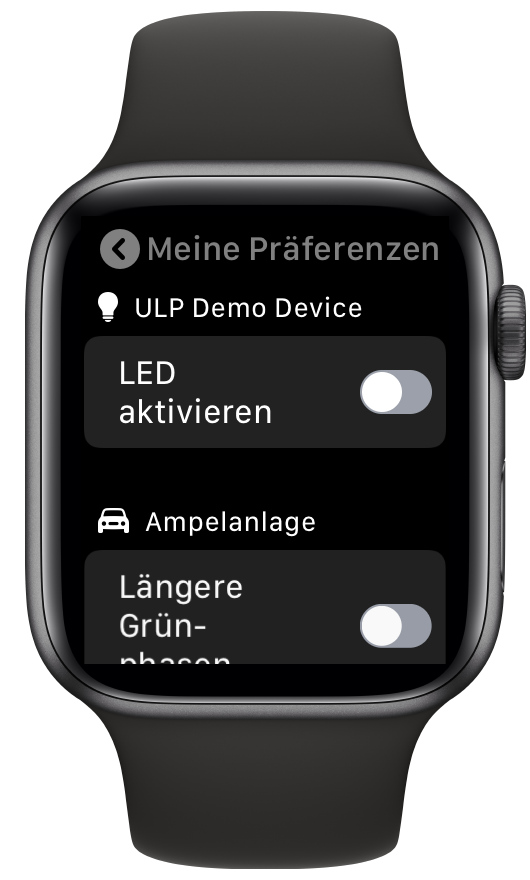
\includegraphics[width=.68\textwidth]{./images/prototype/watchos/prefs.png}
		\caption{\label{fig:app:watchos:prefs}Präferenzen festlegen.}
	\end{figure}
\end{minipage}\hfill
\begin{minipage}{.45\textwidth}
	\begin{figure}[H]
		\centering
		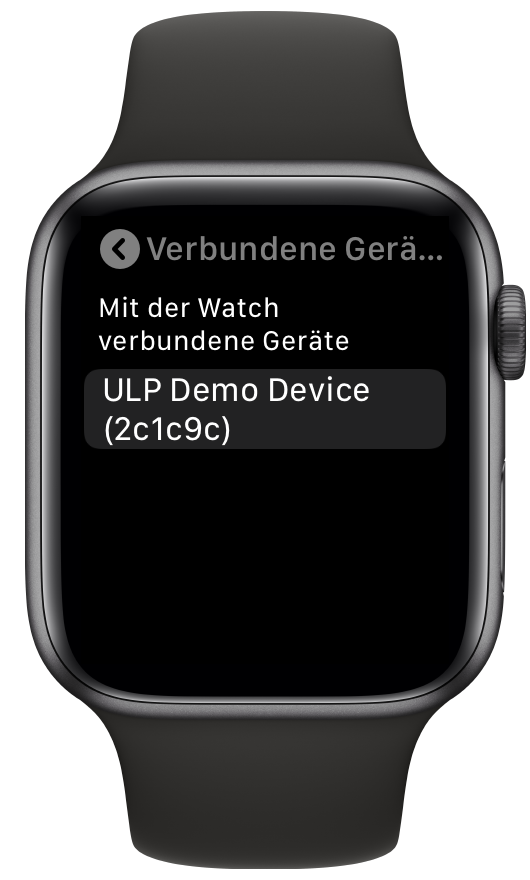
\includegraphics[width=.68\textwidth]{./images/prototype/watchos/connectedTo.png}
		\caption{\label{fig:app:watchos:connectedTo}Verbundene Geräte.}
	\end{figure}
\end{minipage}

    \chapter{Fazit}

Wir haben gesehen, dass es bereits einige Arbeiten gibt, die sich mit UI-Richtlinien für ältere Menschen befassen. Mehrere Arbeiten haben Richtlinien erarbeitet, die befolgt werden können.

Erreichbarkeit sollte von allen Entwicklern im Hinterkopf behalten werden \cite{Diaz-Bossini:2014:Accessibility-to-Mobile-Interfaces}. Mit SwiftUI hat Apple eine einfache Möglichkeit geschaffen, auf einfache Weise adaptive UIs zu programmieren.

Die entwickelte App sollte im nächsten Schritt dann mit einer Zielgruppe auf die Nutzbarkeit hin evaluiert werden.
    
%    \chapter{Finibus Bonorum et Malorum}

Lorem ipsum dolor sit amet, consectetuer adipiscing elit. Nullam et lectus ac lacus bibendum ullamcorper. Sed ante neque, scelerisque eu, sodales quis, elementum nec, risus. Aliquam erat volutpat. Suspendisse potenti. Praesent erat justo, viverra sed, dignissim ut, tempus eget, orci. Morbi luctus ultrices tortor. Maecenas sit amet enim. Morbi facilisis fringilla nunc. Fusce venenatis nunc a nunc. Quisque interdum pretium erat. In mattis feugiat sapien. Aliquam erat volutpat. Proin pellentesque ullamcorper risus. Integer at risus ut velit eleifend sagittis.

\section{In adipiscing purus et purus}

\glqq Vestibulum eu\grqq\ velit \cite{praxisbuch2017} (Zitat aus einem Buch). Donec pharetra feugiat elit. Morbi vitae arcu. Sed dignissim, lectus at ultricies fringilla, mauris mi eleifend mi, nec varius ipsum nunc a enim. Vivamus quis libero a erat varius accumsan. Nullam porttitor, est vitae dignissim eleifend, lacus mi semper justo, elementum imperdiet ante nibh sed nisl. Pellentesque suscipit venenatis ipsum. Suspendisse ultricies elit et neque. Sed risus erat, vehicula eget, vulputate sit amet, viverra sit amet, arcu. Integer malesuada risus vitae est. Donec vulputate, enim a laoreet vehicula, est magna vulputate justo, ut congue sapien mi gravida arcu. Curabitur luctus sapien id orci. Maecenas pulvinar, dolor id placerat convallis, mi metus fringilla enim, eu dignissim urna justo sollicitudin nibh. Vestibulum tellus nisi, nonummy vitae, aliquet a, vehicula et, justo.

Donec viverra tortor non lectus. Vestibulum vel nulla ac sapien tristique imperdiet. Sed neque. Suspendisse porta risus nec mi. Nulla id orci. Boah Alter. Donec nunc dolor, ullamcorper sit amet, imperdiet vitae, blandit et, lacus. Cum sociis natoque penatibus et magnis dis parturient montes, nascetur ridiculus mus. Suspendisse potenti. Ut nibh. Cras enim. Mauris a ligula scelerisque ligula dictum cursus. Proin malesuada massa non nulla. Praesent imperdiet massa eu justo.

%Grafik aus PNG-File - bei dieser Variante darauf achten, dass die Grafik in ausreichender Auflösung vorliegt (so dass auch nach Skalierung >300dpi im Ausdruck erreicht werden)
\begin{figure}[htb]
  \centering
  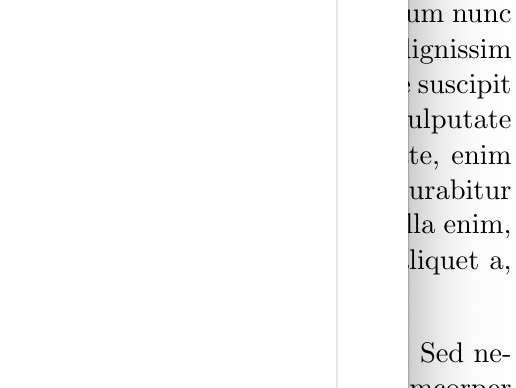
\includegraphics[width=.4\textwidth]{LampFlowchart}\\ % PNG-File
  \caption{Nulla interdum aliquam leo}\label{fig:LampFlowchart}
\end{figure}


Vestibulum ante ipsum primis in faucibus orci luctus et ultrices posuere cubilia Curae (vgl. Abbildung~\ref{fig:LampFlowchart}); Curabitur mauris urna, tincidunt eget, porttitor in, lacinia vel, massa. Integer nonummy, elit at ullamcorper facilisis, massa sem elementum sapien, non malesuada ipsum lacus sed enim. Cras nec eros ut sapien sodales scelerisque. Sed quam. Suspendisse potenti. Nunc eu tortor. Nam nisi arcu, mattis ut, vehicula et, tristique in, erat. Class aptent taciti sociosqu ad litora torquent per conubia nostra, per inceptos hymenaeos. Nullam justo. Integer eget erat at mauris tristique ultrices. Sed ullamcorper vulputate velit. Vivamus blandit erat non erat luctus venenatis. Mauris elementum semper nunc. Cras pellentesque tristique nulla. Pellentesque metus. Mauris semper mi quis pede. Proin vel tellus.

Maecenas euismod, orci in mollis scelerisque, turpis elit lobortis nunc, a venenatis nisl orci quis nibh. Duis tincidunt dictum elit. Nulla sodales est nec nisi. Phasellus consectetuer suscipit urna. Nulla augue. Pellentesque tincidunt pellentesque diam. Etiam iaculis. Cras aliquet metus sed est. Cras egestas, nibh nec commodo suscipit, mauris dolor blandit dolor, id egestas lorem nibh eu nisl. Sed tempor tempor lorem. Donec fringilla luctus quam. Nam metus magna, varius non, tempor eget, rutrum quis, velit. Maecenas sit amet neque id tellus venenatis scelerisque. Donec sed purus. Quisque eu quam a augue consequat consequat.

\section{Etiam blandit molestie ligula}

Proin pharetra ultrices enim. Maecenas dui. Mauris est eros, posuere vitae, sagittis quis, tempus ut, mauris. Fusce congue, augue imperdiet tincidunt volutpat, justo metus tristique lacus, eu ultrices mauris mi ac tellus. Praesent porttitor accumsan erat. Quisque lacinia mollis turpis. Suspendisse potenti. Morbi eu urna vel purus congue accumsan. Aliquam consectetuer nulla nec augue. Nam fringilla nisi nec felis. Donec nibh tellus, consequat quis, cursus sed, vulputate eu, orci. Donec vulputate, elit vel iaculis hendrerit, augue augue congue erat, vel vestibulum tortor dui a diam (vgl. Abbildung~\ref{fig:BurgerFlowchart}). Etiam vel lorem a libero feugiat feugiat. In blandit est a est. Nulla interdum pharetra nulla. Nullam eu ipsum.

%Grafik aus PDF-File - diese Variante ist vorzuziehen, da sie die Einbundung echter Vektorgrafiken ermöglicht
\begin{figure}[htb]
  \centering
 % \includegraphics[scale=.6]{BurgerFlowchart}\\ % PDF-File
  \caption{Donec tempor leo a massa~\cite{praxisbuch2017} (Zitat aus Norm, Handbuch u.ö.)}\label{fig:BurgerFlowchart}
\end{figure}

Quisque ligula orci, accumsan vel, molestie ac, lacinia non, lorem . Fusce nonummy. Cras mattis, elit ac tempor congue, ante arcu porta justo, at rhoncus sapien erat vel dui~\cite{latexbib}. Phasellus vestibulum, turpis non tempor vehicula, quam lacus accumsan dolor, id dictum magna magna eu neque. Sed suscipit placerat odio. Sed et sem. Mauris vel tortor a nisl egestas vulputate. Aliquam facilisis luctus nibh. Maecenas vel lectus sed urna viverra pretium. Aenean malesuada nibh sed ipsum. Fusce vel augue. Mauris eget massa. Class aptent taciti sociosqu ad litora torquent per conubia nostra, per inceptos hymenaeos. Etiam nec justo eu purus ultricies mattis. In leo ante, adipiscing sit amet, ultrices at, ultrices et, nulla. Mauris quis odio. Donec sollicitudin rutrum sapien. Aliquam eget ante a dui euismod porttitor. Donec commodo scelerisque purus. Sed magna.

Cras gravida. Praesent posuere lacus ut tellus. Nunc tempor dapibus urna. Proin sit amet velit ut urna lobortis ultrices. Suspendisse potenti. Maecenas est libero, condimentum in, mattis a, viverra in, sem. Sed nec pede. Fusce risus magna, porta eu, rhoncus vel, facilisis at, risus. Donec commodo viverra neque. Donec ultrices neque vitae justo. Nulla et magna. In condimentum tellus vitae erat. Quisque nec odio.


Nullam consectetuer risus vitae orci. Aliquam fermentum leo sit amet nulla laoreet hendrerit. Maecenas tempus, neque eu posuere vestibulum, pede eros adipiscing augue, pulvinar ullamcorper lectus lectus et tellus. Donec at velit at velit pellentesque sagittis. Vestibulum ultricies ultrices mi. Vestibulum accumsan dictum ligula. Ut lobortis, odio ut semper vehicula, nibh quam semper nisi, sed adipiscing purus lectus et sem. Mauris nisl est, scelerisque ut, ultrices nec, faucibus vitae, nulla. Nulla nisi. Suspendisse potenti. Etiam ultrices commodo odio. Quisque turpis purus, mollis sed, pretium quis, volutpat et, neque. Nam a sapien eget neque consectetuer ornare. Pellentesque felis metus, pellentesque quis, volutpat rhoncus, laoreet id, nunc. Duis egestas, felis et luctus vestibulum, velit nunc luctus felis, non tempor justo ligula et nulla. Vestibulum, Abbildung~\ref{fig:tabelle}, est. Nulla aliquam eleifend justo.

%Tabellen im Regelfall auch in eine Figure-Umgebung setzen - Verwendung von Table-Umgebung lohnt nur bei sehr vielen Tabellen
\begin{figure}[htb]
  \centering
  \begin{tabular}{|l|c|}
    \hline
    \textbf{tempus} & \textbf{risus} \\ \hline
    ultrices & pellentesque \\
    rhoncus & egestas \\
    \hline
  \end{tabular}
  \caption{Aliquam fermentum}\label{fig:tabelle}
\end{figure}

Class aptent taciti sociosqu ad litora torquent per conubia nostra, per inceptos hymenaeos. Lorem ipsum dolor sit amet, consectetuer adipiscing elit. Sed auctor urna quis turpis. Suspendisse potenti. Donec tempus gravida ante. Nulla magna velit, condimentum et, pharetra sollicitudin, tincidunt et, nibh. Donec tincidunt, leo a facilisis consectetuer, quam diam cursus nibh, vitae porttitor lacus dolor in lacus. Nulla id nulla in dolor adipiscing posuere. Proin sagittis mattis dui. Maecenas neque arcu, ornare a, gravida et, posuere ut, massa. Donec congue odio ac enim. Nam malesuada sapien sit amet ante. Donec ullamcorper pulvinar dolor. Fusce posuere tellus.

\section{Ut venenatis mi id orci}

Class aptent taciti sociosqu ad litora torquent per conubia nostra, per inceptos hymenaeos. Ut quam odio, luctus gravida, aliquam eu, fringilla a, nulla. Nulla facilisi. Aliquam tincidunt porta urna. Nulla facilisi. Cras pellentesque cursus risus. Quisque semper imperdiet ante. Donec erat magna, sagittis vitae, convallis ut, tincidunt et, lectus. Mauris vulputate tincidunt mi. Integer diam enim, mollis non, dignissim non, faucibus eu, enim. Aliquam erat volutpat. Sed facilisis sagittis massa. Vivamus vel neque. Donec eu mi. Aenean lobortis. Nullam pulvinar. Mauris vel lorem vel dolor semper volutpat. Nam posuere blandit arcu.

\endinput

%    \chapter{Finibus Bonorum et Malorum 2}

TBC\ldots


% ---------------------------------------------------------------
\backmatter
	\chapter{Abkürzungsverzeichnis}
\begin{acronym}[BT Classic]%[<längstes Akronym hier>]
	\acro{BLE}{Bluetooth Low Energy}
	\acro{BT Classic}{Bluetooth Classic}
	\acro{CB}{Core Bluetooth}
	\acro{CCCD}{Client Characteristic Configuration Descriptor}
	\acro{SDK}{Software Development Kit}
%	 Wird verwendet, um Software zu entwickeln.
	\acro{MWABP}{Mobile Web Application Best Practices}
	\acro{MWBP}{Mobile Web Best Practices}
	\acro{SMASH}{SMArtphone's uSability Heuristics}
	\acro{SSO}{Smartes städtebauliches Objekt}
	\acrodefplural{SSO}{smarte städtebauliche Objekte}
	\acro{UI}{User Interface}
	\acro{UUID}{Universally Unique Identifier}
	\acro{UX}{User Experience}
	\acro{W3C}{World Wide Web Consortium}
	\acro{WAI}{Web Accessibility Initiative}
	\acro{WCAG}{Web Content Accessibility Guidelines}
\end{acronym}
    \listoffigures
    \listoftables

    \printbibliography[title=Literaturverzeichnis, nottype=online]
    \printbibliography[title=Quellenverzeichnis, type=online]
    Alle Links im Quellenverzeichnis wurden am 2. Juni 2020 auf Verfügbarkeit überprüft.

    \newpage

\thispagestyle{empty}

\begin{large}

\vspace*{2cm}

\noindent
Hiermit versichere ich, die vorliegende Arbeit selbständig und ohne fremde Hilfe verfasst, die Zitate ordnungsgemäß gekennzeichnet und keine anderen, als die im Literatur/Schriftenverzeichnis angegebenen Quellen und Hilfsmittel benutzt zu haben.\\[2em]
\noindent
Ferner habe ich vom Merkblatt über die Verwendung von studentischen Abschlussarbeiten Kenntnis genommen und räume das einfache Nutzungsrecht an meiner Bachelorarbeit der Universität der Bundeswehr München ein.

\vspace{2cm}

\noindent
Neubiberg, den 2. Juni 2020

\vspace{3cm}

\hfill
\begin{minipage}{8cm}
\centering
\begin{Large}
{\fontfamily{augie}\fontseries{m}\fontshape{n}\selectfont Henning Hontheim}\\
\end{Large}
\hspace*{0cm}
\dotfill\\
\hspace*{0cm}
\textit{(Henning Hontheim)}
\end{minipage}
\end{large}
\end{document}
